%%%%%%%% ICML 2026 EXAMPLE LATEX SUBMISSION FILE %%%%%%%%%%%%%%%%%

\documentclass{article}

% Recommended, but optional, packages for figures and better typesetting:
\usepackage{microtype}
\usepackage{graphicx}
\usepackage{subcaption}
\usepackage{multirow,multicol}
\usepackage{booktabs} % for professional tables
\usepackage{algpseudocode}

% hyperref makes hyperlinks in the resulting PDF.
% If your build breaks (sometimes temporarily if a hyperlink spans a page)
% please comment out the following usepackage line and replace
% \usepackage{icml2026} with \usepackage[nohyperref]{icml2026} above.
\usepackage{hyperref}

\usepackage{tikz}
\usetikzlibrary{arrows.meta, positioning}

% Attempt to make hyperref and algorithmic work together better:
%\newcommand{\theHalgorithm}{\arabic{algorithm}}

% Use the following line for the initial blind version submitted for review:
\usepackage{icml2026}

% For preprint, use
% \usepackage[preprint]{icml2026}

% If accepted, instead use the following line for the camera-ready submission:
% \usepackage[accepted]{icml2026}

\usepackage{amsmath}
\usepackage{amssymb}
\usepackage{mathtools}
\usepackage{amsthm}


% if you use cleveref..
\usepackage[capitalize,noabbrev]{cleveref}

%%%%%%%%%%%%%%%%%%%%%%%%%%%%%%%%
% THEOREMS
%%%%%%%%%%%%%%%%%%%%%%%%%%%%%%%%
\theoremstyle{plain}
\newtheorem{theorem}{Theorem}[section]
\newtheorem{proposition}[theorem]{Proposition}
\newtheorem{lemma}[theorem]{Lemma}
\newtheorem{corollary}[theorem]{Corollary}
\theoremstyle{definition}
\newtheorem{definition}[theorem]{Definition}
\newtheorem{assumption}[theorem]{Assumption}
\theoremstyle{remark}
\newtheorem{remark}[theorem]{Remark}

% Todonotes is useful during development; simply uncomment the next line
%    and comment out the line below the next line to turn off comments

%\usepackage[disable,textsize=tiny]{todonotes}
\usepackage[textsize=tiny]{todonotes}

% The \icmltitle you define below is probably too long as a header.
% Therefore, a short form for the running title is supplied here:
\icmltitlerunning{PaCT: Parallel Continuous Thought for Reasoning in Large Language Models}

\begin{document}
\twocolumn[
  %\icmltitle{Thinking in Parallel: Accelerating Continuous Latent Reasoning in Large Language Models}
  \icmltitle{PaCT: Parallel Continuous Thought for Reasoning in Large Language Models}

  % It is OKAY to include author information, even for blind submissions: the
  % style file will automatically remove it for you unless you've provided
  % the [accepted] option to the icml2026 package.

  % List of affiliations: The first argument should be a (short) identifier you
  % will use later to specify author affiliations Academic affiliations
  % should list Department, University, City, Region, Country Industry
  % affiliations should list Company, City, Region, Country

  % You can specify symbols, otherwise they are numbered in order. Ideally, you
  % should not use this facility. Affiliations will be numbered in order of
  % appearance and this is the preferred way.
  \icmlsetsymbol{equal}{*}

  \begin{icmlauthorlist}
    \icmlauthor{Firstname1 Lastname1}{equal,yyy}
    \icmlauthor{Firstname2 Lastname2}{equal,yyy,comp}
    \icmlauthor{Firstname3 Lastname3}{comp}
    \icmlauthor{Firstname4 Lastname4}{sch}
    \icmlauthor{Firstname5 Lastname5}{yyy}
    \icmlauthor{Firstname6 Lastname6}{sch,yyy,comp}
    \icmlauthor{Firstname7 Lastname7}{comp}
    %\icmlauthor{}{sch}
    \icmlauthor{Firstname8 Lastname8}{sch}
    \icmlauthor{Firstname8 Lastname8}{yyy,comp}
    %\icmlauthor{}{sch}
    %\icmlauthor{}{sch}
  \end{icmlauthorlist}

  \icmlaffiliation{yyy}{Department of XXX, University of YYY, Location, Country}
  \icmlaffiliation{comp}{Company Name, Location, Country}
  \icmlaffiliation{sch}{School of ZZZ, Institute of WWW, Location, Country}

  \icmlcorrespondingauthor{Firstname1 Lastname1}{first1.last1@xxx.edu}
  \icmlcorrespondingauthor{Firstname2 Lastname2}{first2.last2@www.uk}

  % You may provide any keywords that you find helpful for describing your
  % paper; these are used to populate the "keywords" metadata in the PDF but
  % will not be shown in the document

  \icmlkeywords{Machine Learning, ICML}

  \vskip 0.2in

  \teaser{
    \centering
    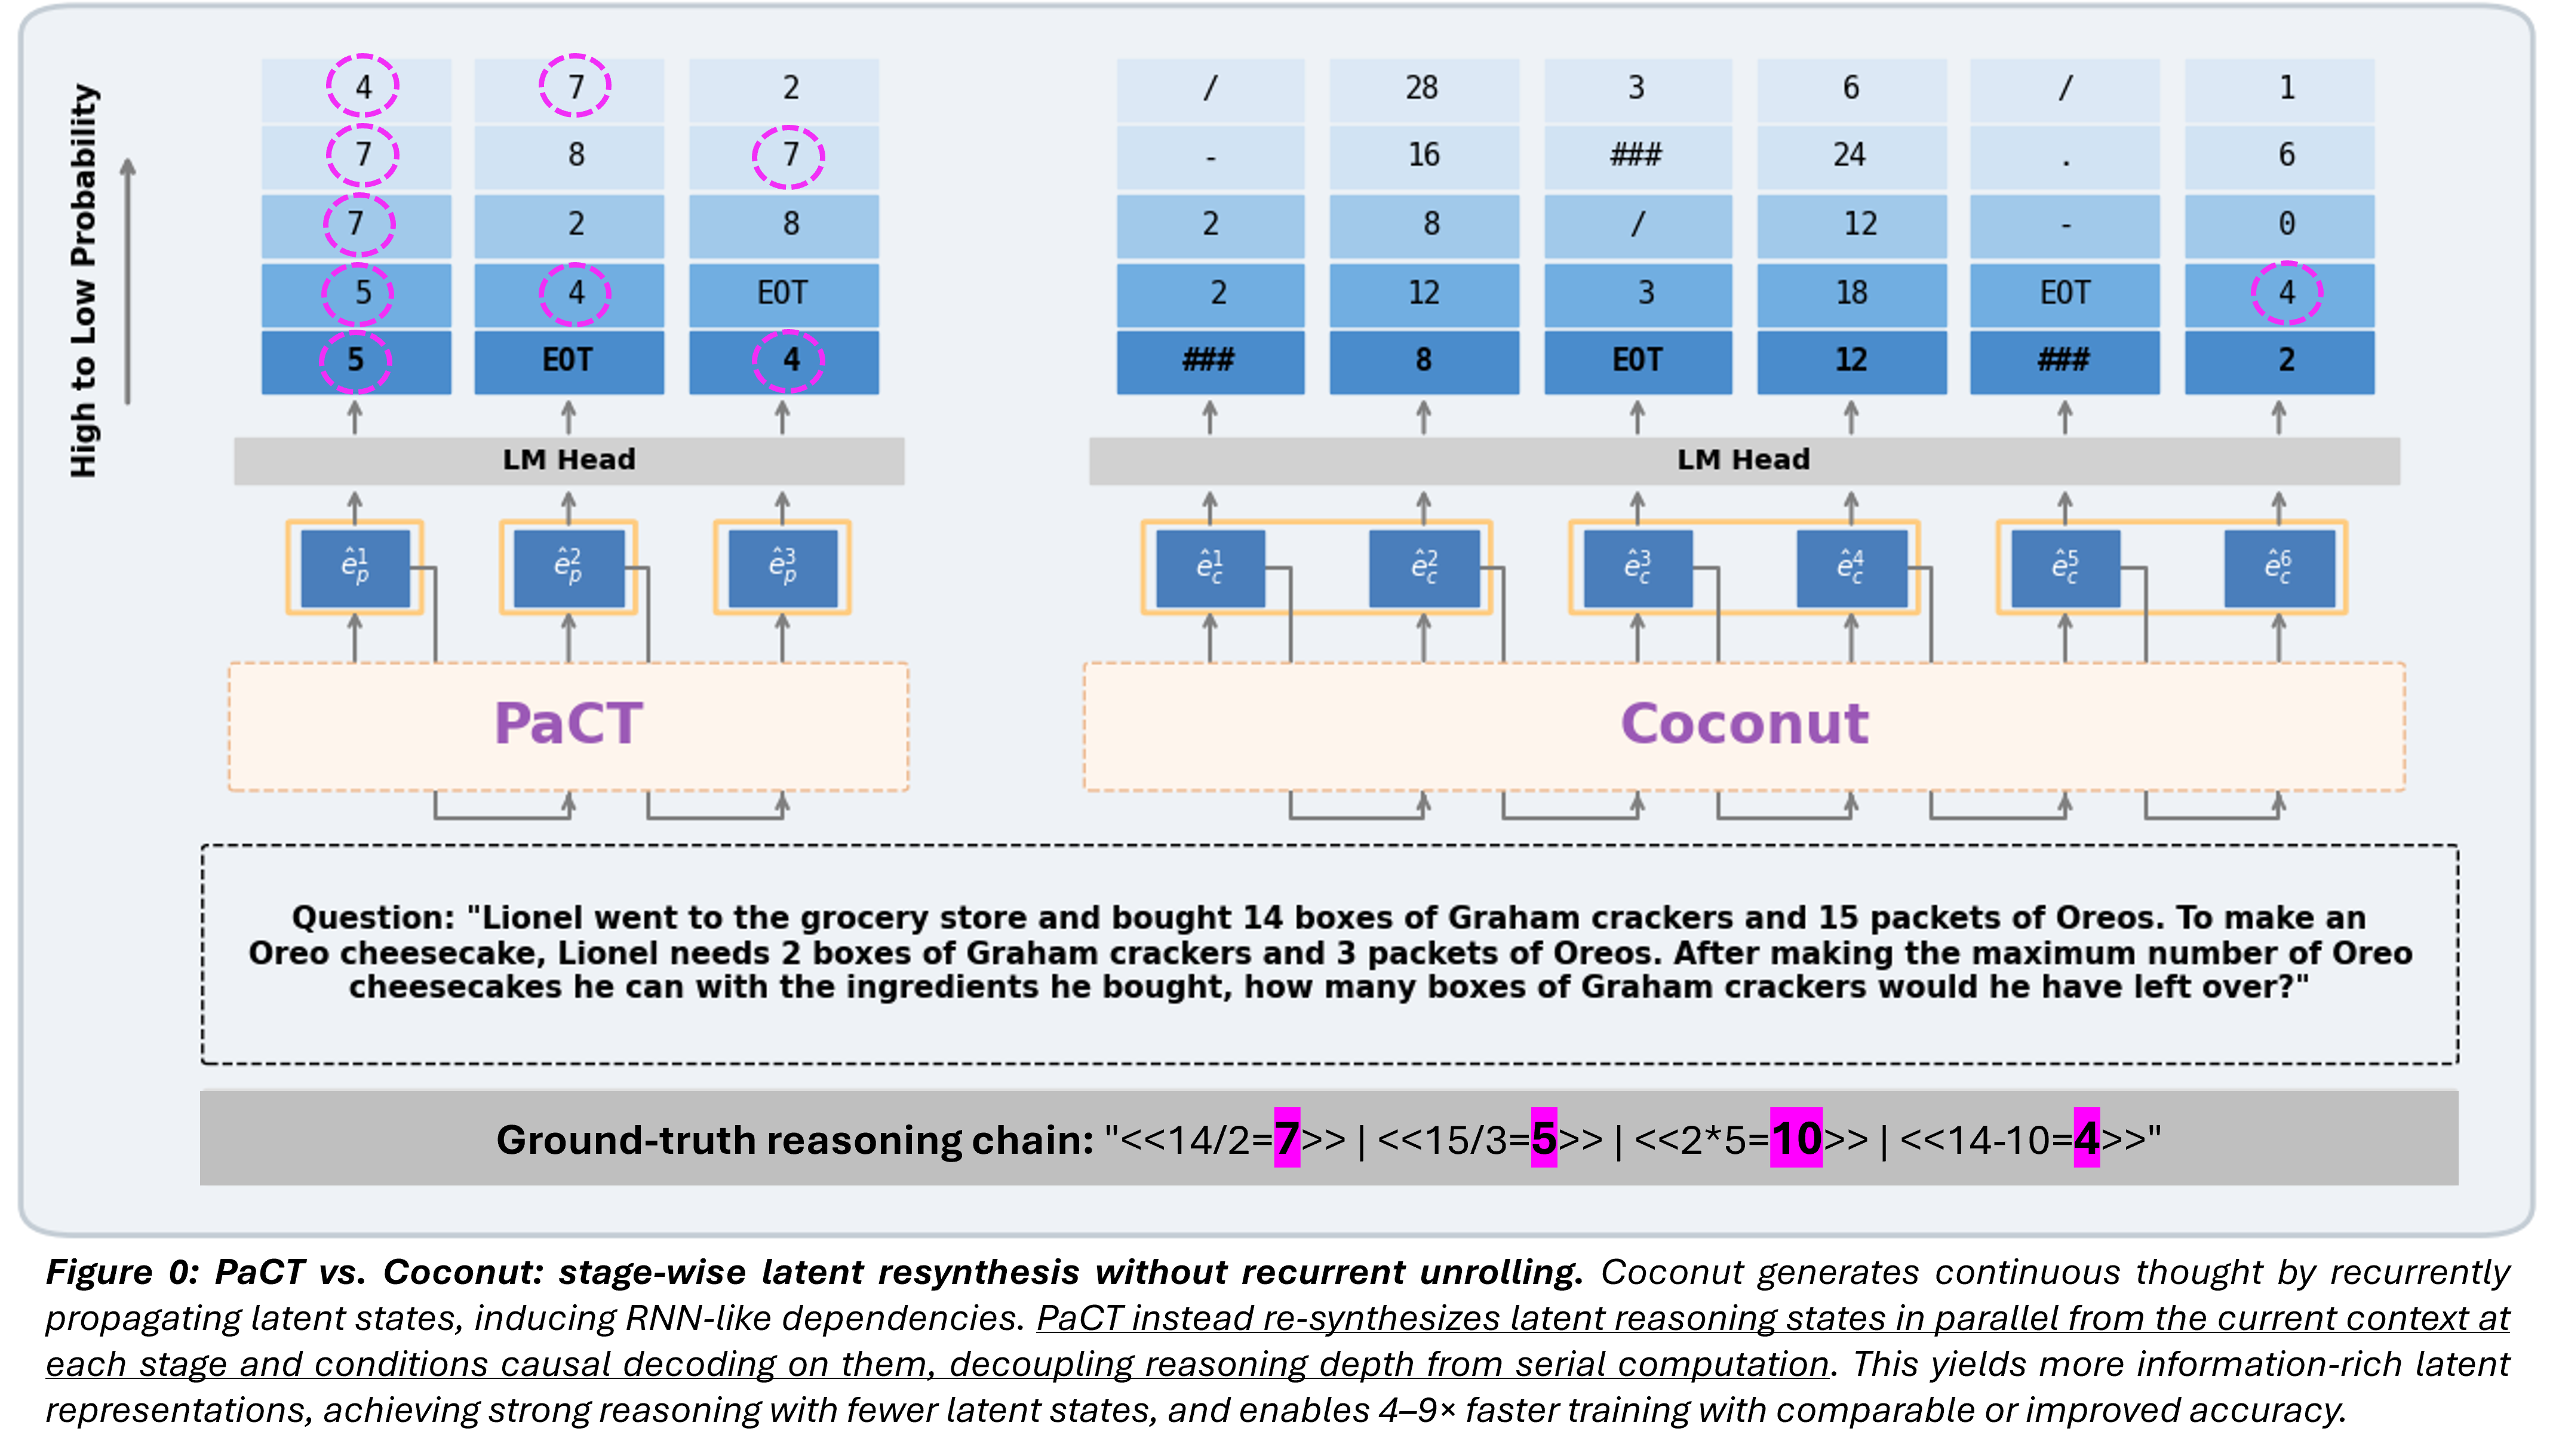
\includegraphics[width=1\textwidth]{imgs/compare_pact_coconut.png}
    \caption{\textit{Figure 0: Comparison of latent token decoding between PaCT and Coconut models on the Graham crackers problem. The grid shows the top-5 token predictions at each latent step, ordered from high to low probability. PaCT uses only 3 latent steps while Coconut uses 6 latent steps yet obtains adequate decoded reasoning. PaCT’s parallelism of latent tokens, reduced count, and information richness makes our method compute efficient.}}
    \label{fig:teaser}
    \vspace{-2mm}
  }

]


% this must go after the closing bracket ] following \twocolumn[ ...

% This command actually creates the footnote in the first column listing the
% affiliations and the copyright notice. The command takes one argument, which
% is text to display at the start of the footnote. The \icmlEqualContribution
% command is standard text for equal contribution. Remove it (just {}) if you
% do not need this facility.

% Use ONE of the following lines. DO NOT remove the command.
% If you have no special notice, KEEP empty braces:
%\printAffiliationsAndNotice{}  % no special notice (required even if empty)
% Or, if applicable, use the standard equal contribution text:
% \printAffiliationsAndNotice{\icmlEqualContribution}

% \teaser{
 
%  \centering
%     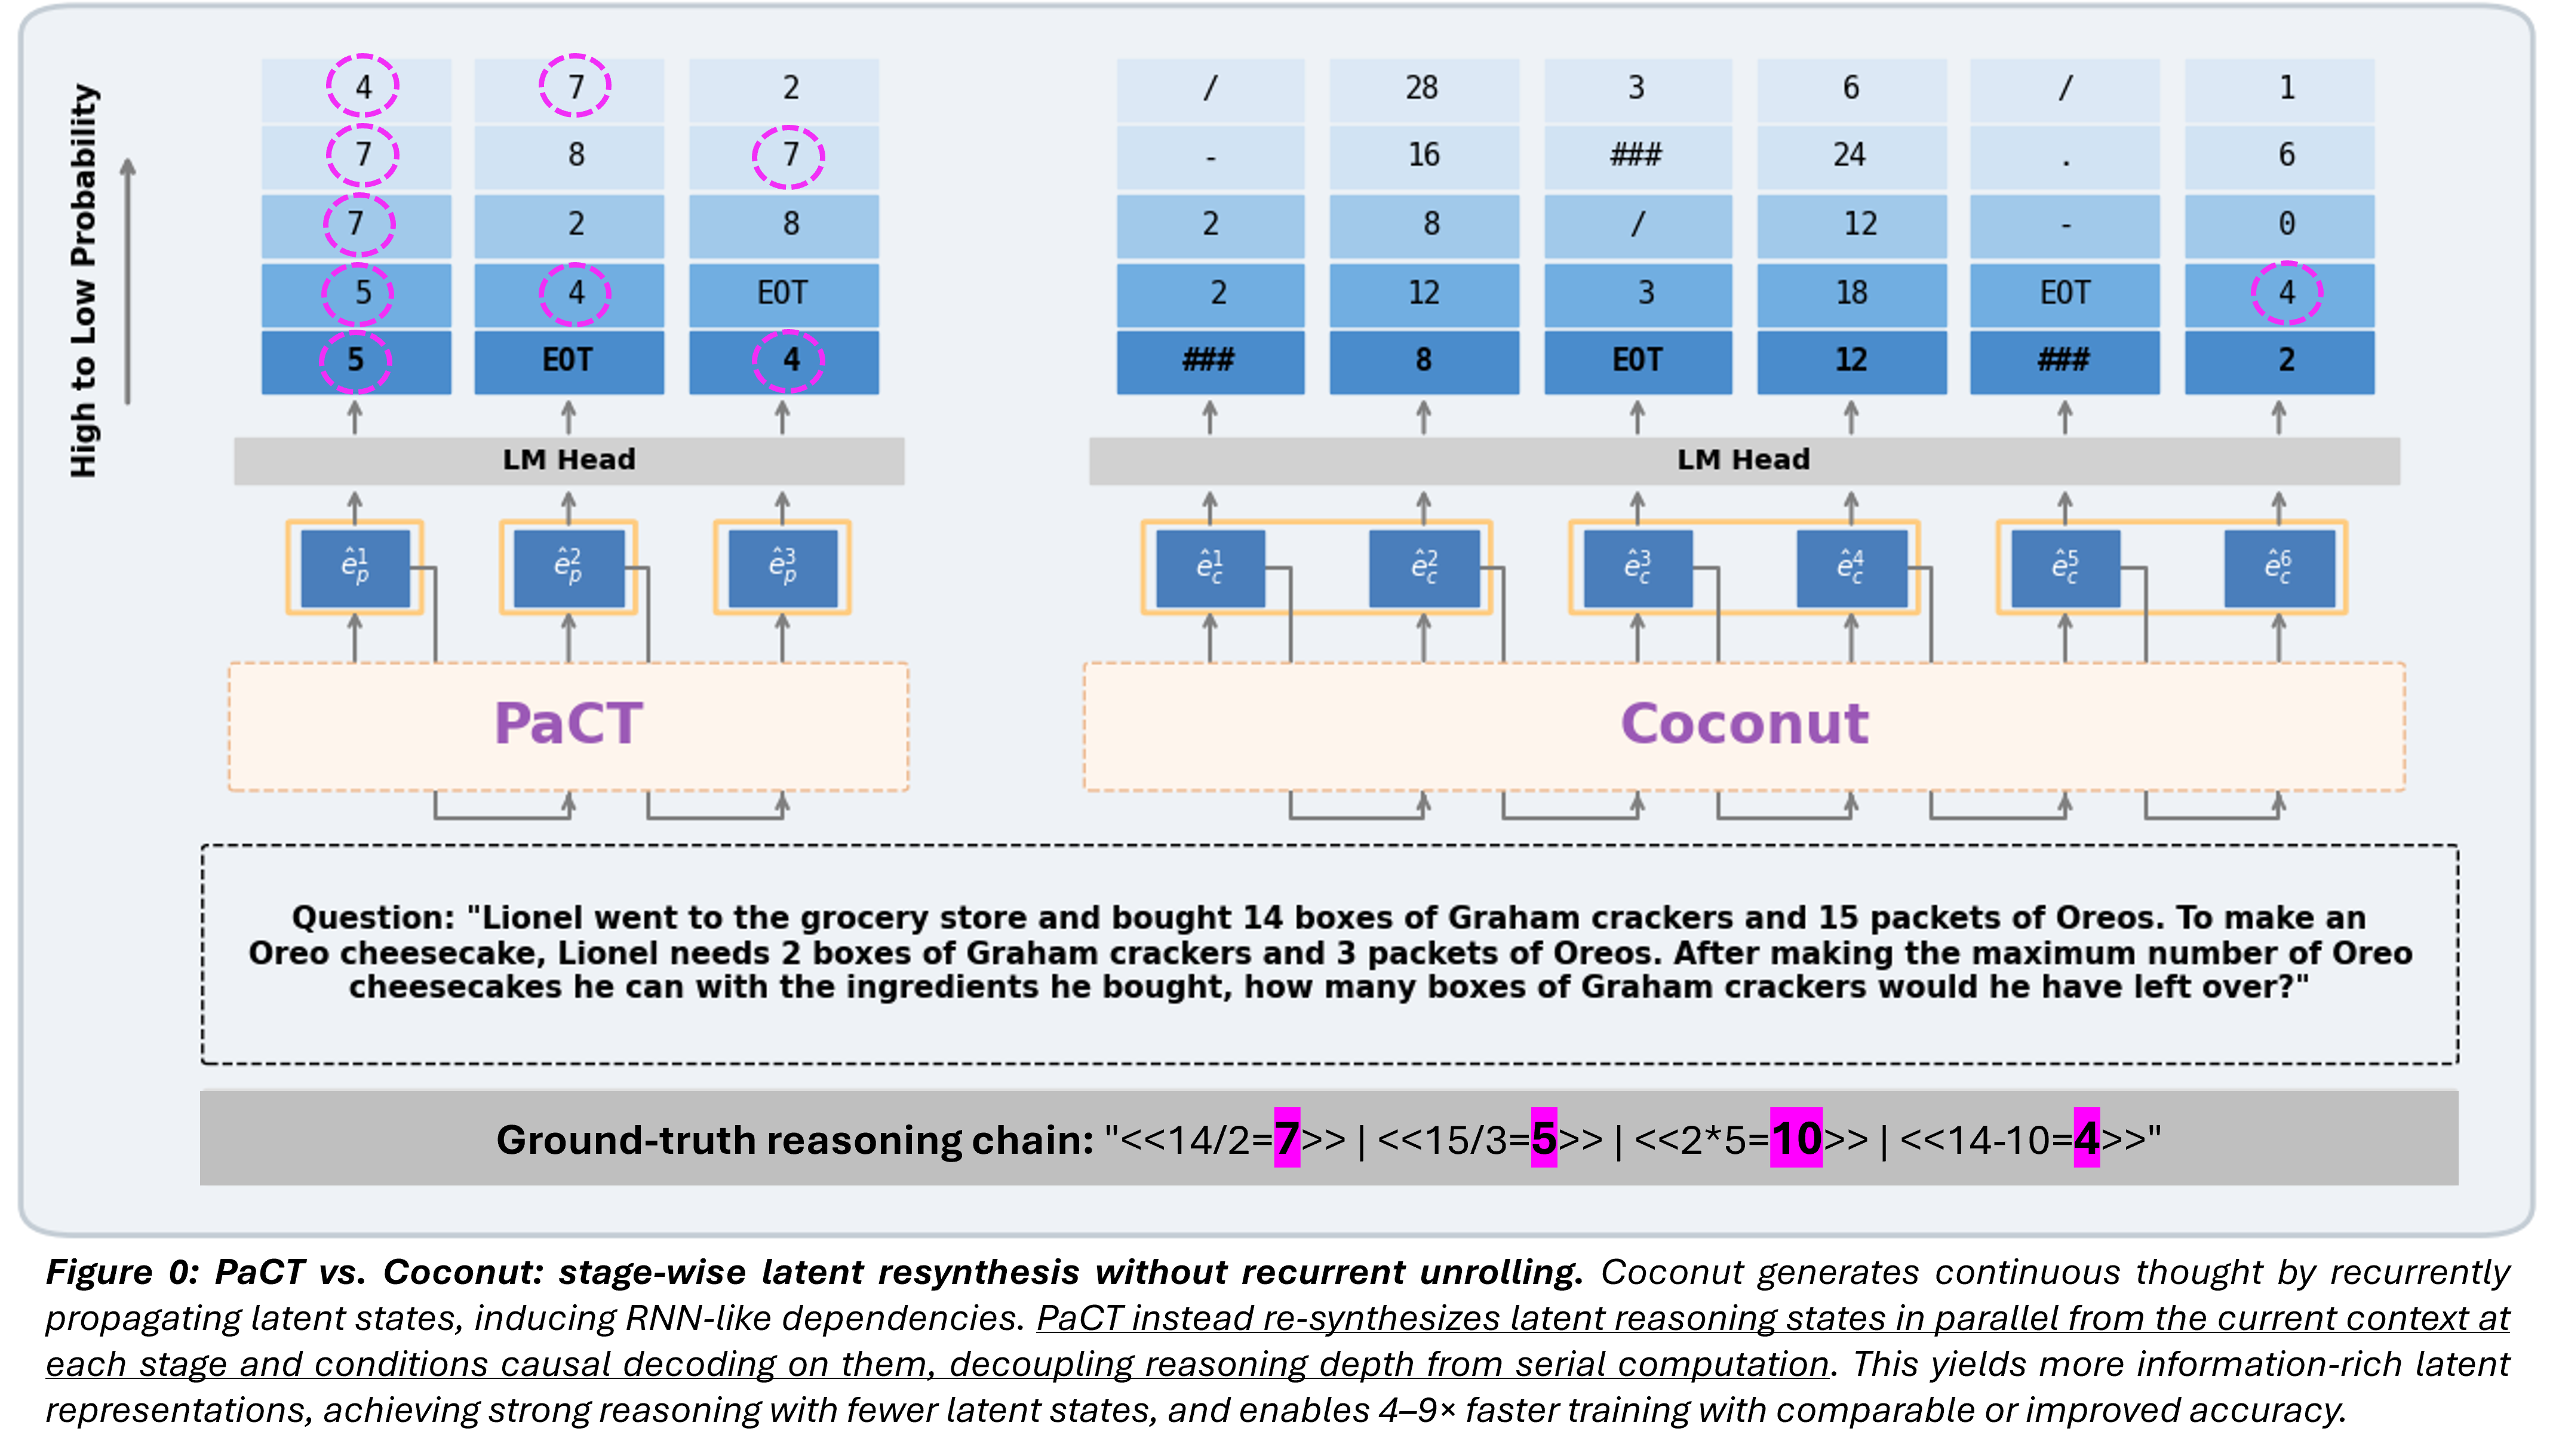
\includegraphics[width=\textwidth]{imgs/compare_pact_coconut.png}
%     \caption{Comparison of latent token decoding between PaCT and Coconut models on the Graham crackers problem. The grid shows the top-5 token predictions at each latent step, ordered from high to low probability. PaCT uses only 3 latent steps while Coconut uses 6 latent steps yet obtains adequate decoded reasoning. PaCTäs parallelism of latent tokens, reduced count, and information rich makes our method compute efficient.}
%     \label{fig:pact_coconut_comparison}
% \label{fig:teaser}
% }



% \begin{figure*}[t]
%     \centering
%     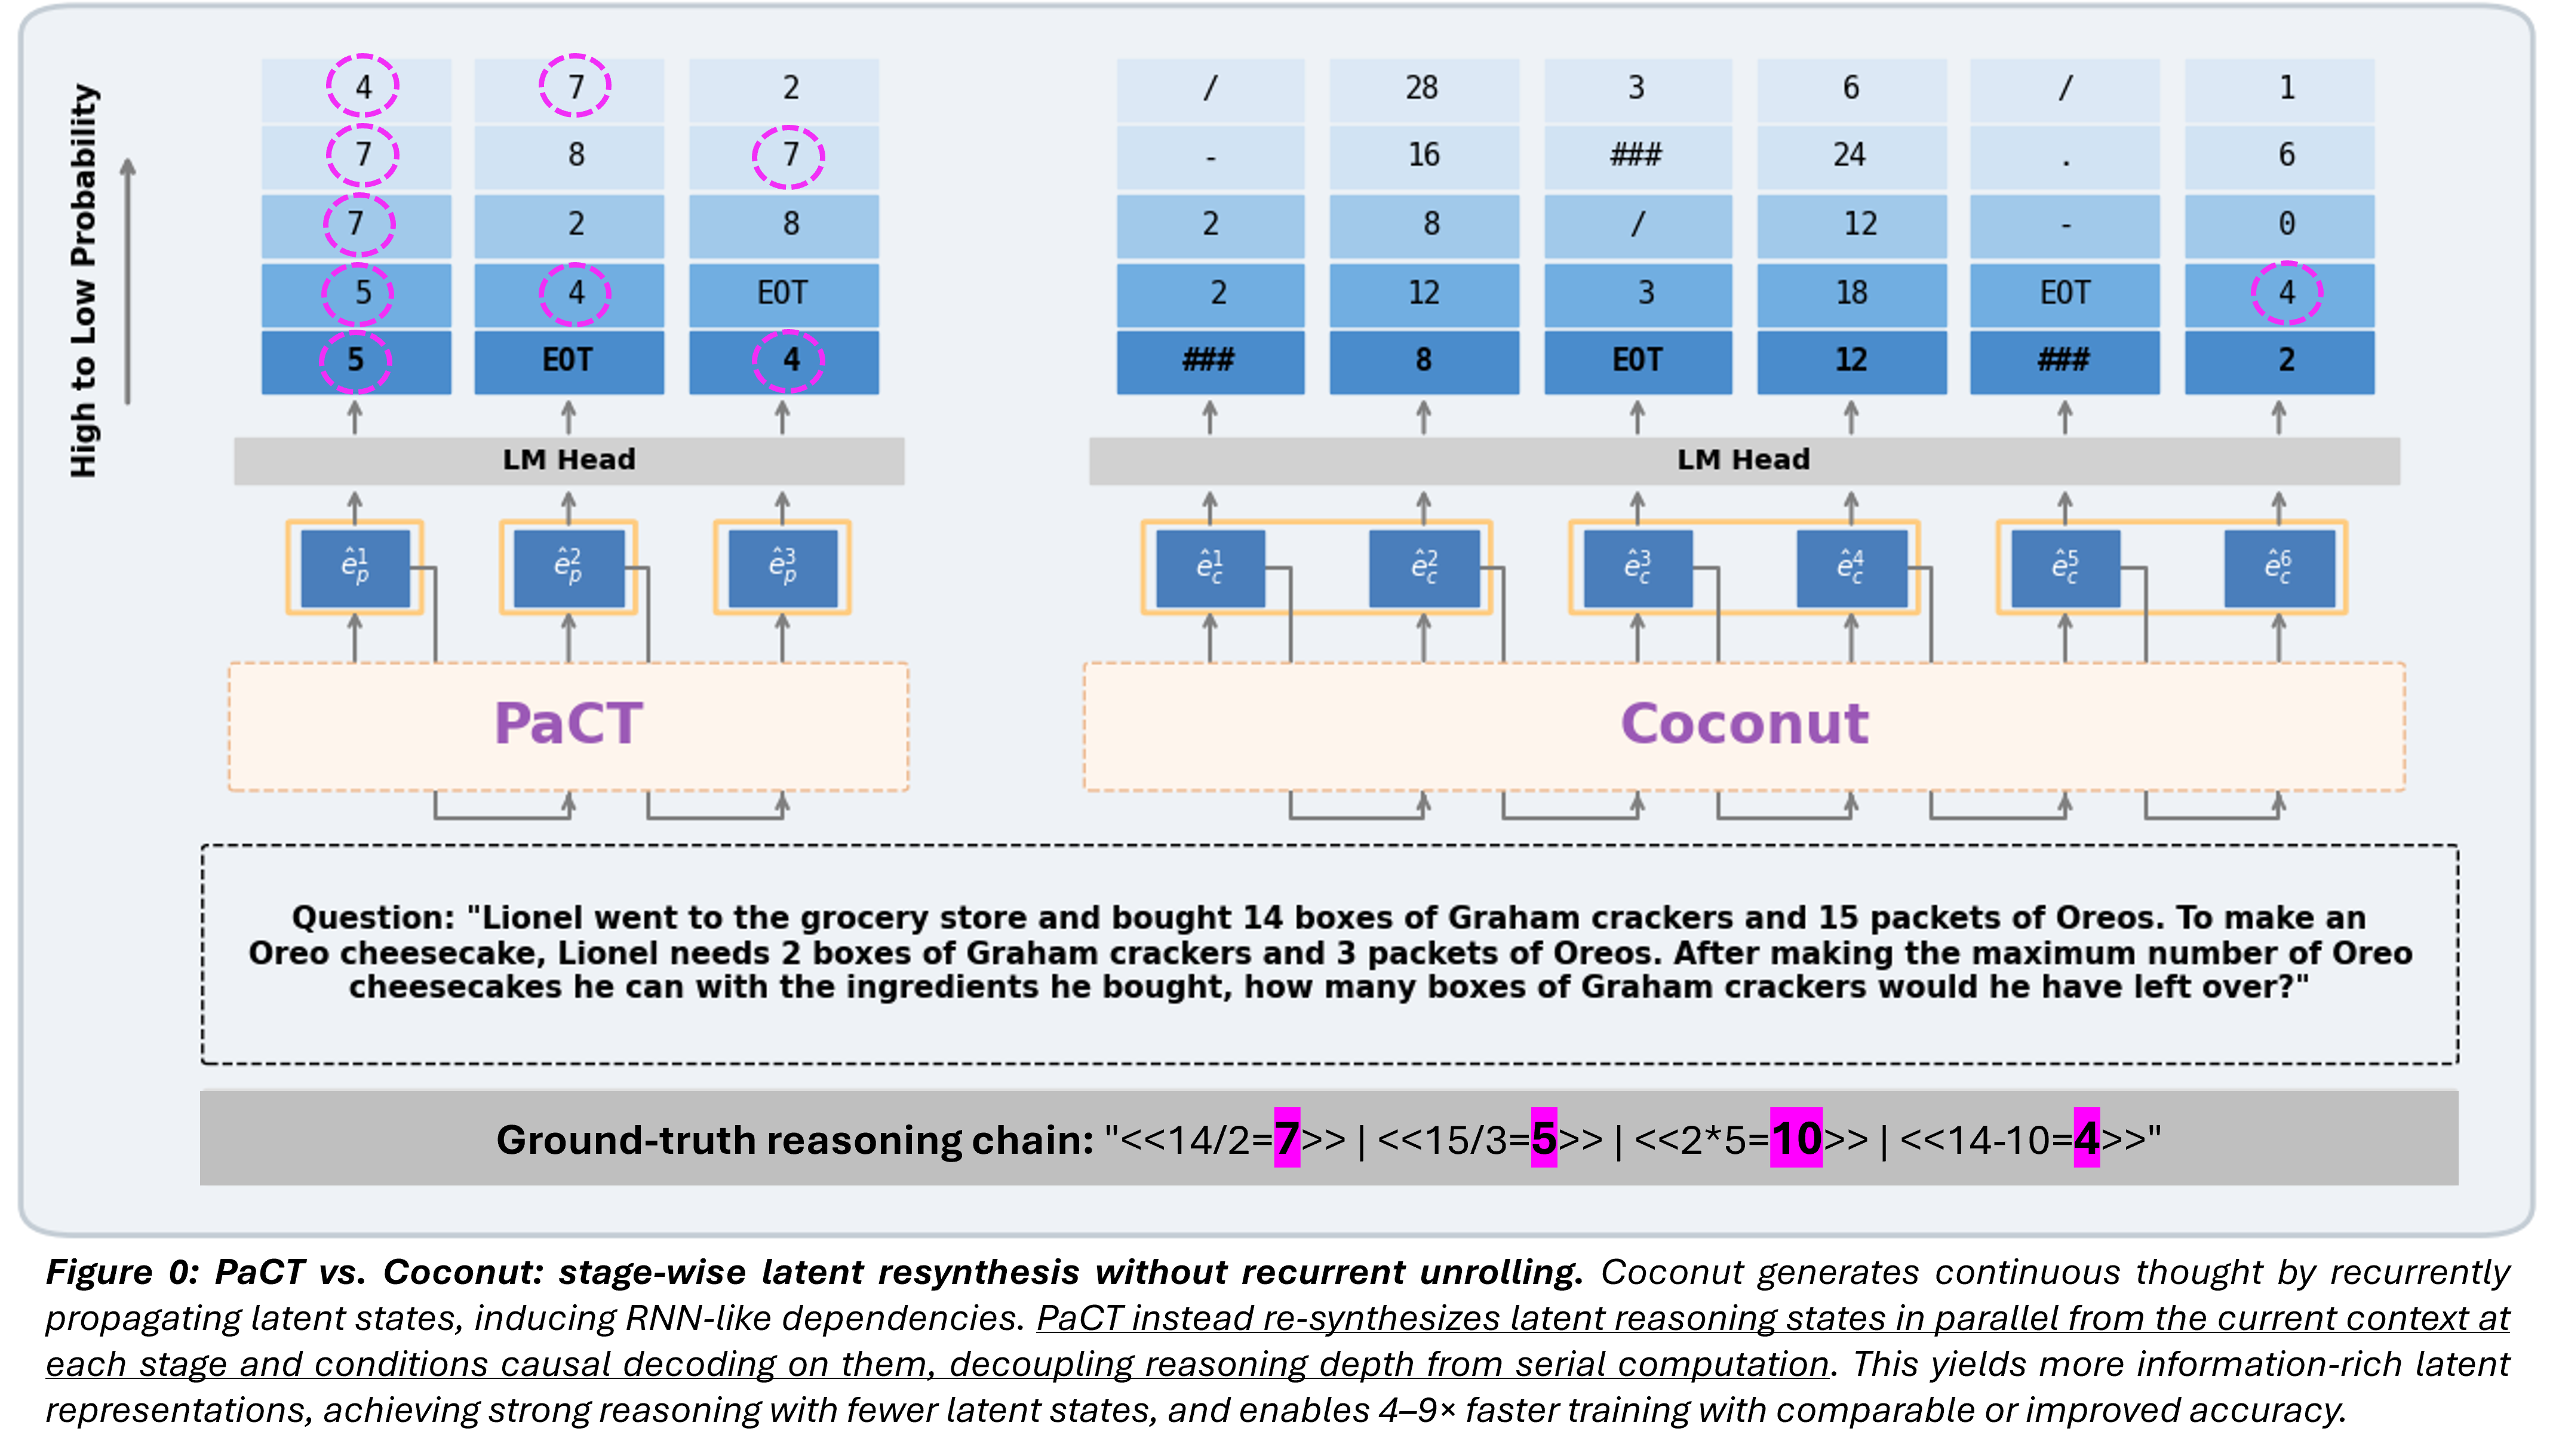
\includegraphics[width=\textwidth]{imgs/compare_pact_coconut.png}
%     \caption{Comparison of latent token decoding between PaCT and Coconut models on the Graham crackers problem. The grid shows the top-5 token predictions at each latent step, ordered from high to low probability. PaCT uses only 3 latent steps while Coconut uses 6 latent steps yet obtains adequate decoded reasoning. PaCTäs parallelism of latent tokens, reduced count, and information rich makes our method compute efficient.}
%     \label{fig:pact_coconut_comparison}
% \end{figure*}

\begin{abstract}
Large language models (LLMs) typically reason in the language space, expressing intermediate computation as chains
of thought (CoT). While effective, this ties reasoning to sequential text token generation, where many tokens primarily ensure textual coherence without directly contributing to the underlying reasoning process, and the cost of reasoning scales with the length of the generated trace. Recent works explore continuous latent reasoning by replacing portions of CoT with internal states by relying on recurrent latent unrolling, introducing long serial dependencies inside the Transformer, and limiting hardware parallelism.
We introduce \emph{Parallel Continuous Thought} (PaCT), which eliminates recurrent unrolling by organizing latent reasoning
into stages. At each stage, PaCT synthesizes a set of latent reasoning states \emph{in parallel} using a learnable query
codebook and cross-attention to the current context, refines them via bidirectional interaction within the stage, and
conditions standard causal decoding through a strictly causal interface. PaCT challenges the assumption that continuous
latent reasoning must rely on latent state propagation, showing that reasoning depth can instead be achieved through
repeated, context-grounded latent resynthesis.
Empirically, PaCT trains substantially faster than recurrent latent unrolling while matching or improving reasoning performance
across diverse settings and model scales. The analyses demonstrate that the stages contribute meaningfully to the final predictions,
encode distinct information across stages, and stabilize the internal dynamics earlier during reasoning. Our code and model weights are available at \href{https://anonymous.4open.science/r/pact-576C/}{PaCT}.
\begin{figure}[t]
  \centering
  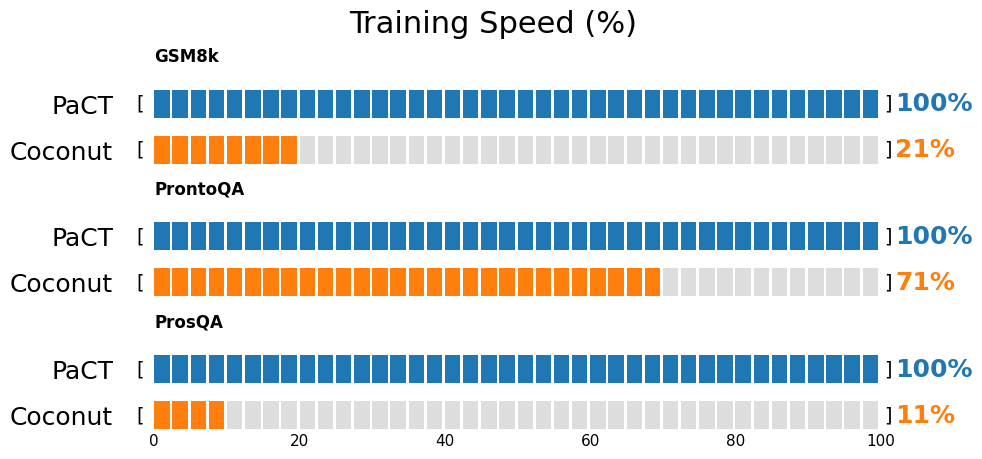
\includegraphics[width=0.65 \linewidth]{imgs/intro_diagram.png}
  \caption{\textbf{PaCT vs.\ Coconut: training speed comparison.}}
  \label{fig:concept_diagram_intro}
  \vspace{-5mm}
\end{figure}
\end{abstract}



% Chain of Continuous Thought (Coconut) enables reasoning in continuous latent space but relies on sequential latent unrolling, which limits computational efficiency. We propose Parallel Continuous Thought (PaCT), which synthesizes latent representations in parallel using a learnable codebook and cross-attention to textual context. PaCT preserves causal decoding while reducing serial computation, achieving comparable or improved reasoning performance with substantially lower training cost.

% \textcolor{red}{Gautam - form novelty perspective following is the statement use it - It aligns very well with introduction, contri, conclusive remarks.}
% \textcolor{blue}{PaCT challenges the assumption that continuous latent reasoning must rely on latent state propagation, showing that reasoning depth can instead be achieved through repeated, context-grounded latent resynthesis.}

% Recent work on Chain of Continuous Thought (Coconut) has shown that large language models can reason effectively in a continuous latent space rather than through explicit language tokens, enabling emergent search behaviors during problem-solving. However, the original formulation generates latent representations sequentially—feeding hidden states back one at a time as subsequent input embeddings—creating a computational bottleneck that limits training efficiency. We introduce \textbf{Parallel Continuous Thought (PaCT)}, a reformulation that replaces sequential latent generation with parallel synthesis via a learnable codebook and cross-attention mechanism. Our approach maintains a set of learnable query vectors that attend to the preceding hidden state context, enabling the simultaneous generation of multiple latent embeddings per reasoning iteration. This architectural modification preserves the model's capacity to reason in continuous latent space while enabling bidirectional attention within each iteration. Experiments on mathematical and logical reasoning benchmarks demonstrate that our method matches or exceeds the accuracy of the original Coconut while achieving a 4-9x reduction in training time. Our results show that efficient parallel latent generation does not compromise reasoning quality, opening pathways for scaling continuous thought reasoning to larger models and more complex tasks.
\end{abstract}
\section{Introduction}
Large language models (LLMs) have recently demonstrated strong multi-step reasoning capabilities when prompted to generate explicit chains of thought (CoT), in which intermediate reasoning steps are expressed as natural language tokens prior to producing a final answer \cite{wei2022chain}. While effective, this paradigm tightly couples reasoning to the discrete token space of language, forcing models to externalize internal computation through sequential text generation. Language tokens, however, are optimized for communication rather than for the core requirements of reasoning such as abstraction, conceptualization, and computation \cite{fedorenko2024language,amalric2019distinct,monti2007functional,monti2009boundaries,monti2012thought,fedorenko2011functional}. Moreover, autoregressive decoding commits to a single partial trajectory token by token, and the computational cost of reasoning scales linearly with the number of generated tokens \cite{saparov2022language}. These constraints make detailed reasoning both expensive and inherently sequential.

A substantial body of work has sought to alleviate these issues through improved prompting strategies and decoding-time search. Techniques such as decomposed prompting \cite{khot2022decomposed}, least-to-most prompting \cite{zhou2022least}, self-consistency and guided beam-style decoding \cite{xie2023self}, and tree-based search over reasoning trajectories \cite{yao2023tree} improve robustness by exploring or aggregating multiple textual reasoning paths. Related approaches introduce test-time deliberation signals that encourage models to ``think'' before committing to an answer \cite{zelikman2024quiet}. Despite their success, these methods operate entirely in token space and therefore inherit its fundamental limitation: each reasoning step must still be generated, evaluated, and committed sequentially. As a result, they improve exploration within the same substrate rather than enabling more abstract or information-dense internal computation.

Recent work has therefore explored shifting reasoning from explicit language tokens into the model’s continuous hidden state space. \emph{Chain of Continuous Thought} (Coconut) introduced the idea of replacing segments of the textual chain-of-thought with continuous latent representations that are never decoded as language and are trained implicitly through their effect on final answer likelihood \cite{hao2024training}. Empirically, Coconut demonstrates that models trained in this manner can exhibit emergent search behaviors resembling breadth-first exploration while requiring fewer explicit reasoning tokens. Complementing this empirical evidence, theoretical analyses show that continuous latent representations can be strictly more expressive than discrete token sequences: \emph{Reasoning by Superposition} proves that a single latent step can encode superpositions of multiple candidate reasoning states that would require sequential exploration in token space \cite{zhu2025reasoning}. Together, these results establish continuous latent reasoning as a promising alternative substrate for complex reasoning.

Despite this promise, existing methods of continuous latent reasoning suffer from a critical structural limitation. In Coconut, continuous thoughts are generated \emph{sequentially}: each latent vector is produced by feeding the previous hidden state back as the next input embedding \cite{hao2024training}. This design introduces a recurrent unrolling within the Transformer, reinstating an RNN-like dependency structure and causing the critical path length to grow linearly with the number of latent steps. Consequently, training becomes substantially slower, hardware parallelism is poorly utilized, and optimization stability degrades as latent depth or model size increases, as gradients must propagate through a long sequence of dependent latent states, causing compounding of early representational instabilities.

Importantly, this recurrent structure imposes not only a computational bottleneck but also a representational one. When latent thoughts are generated by recursively transforming prior latent states, each latent must accumulate and carry forward information from earlier steps, as future computation has access only to the most recent latent. The absence of an explicit stage boundary encourages successive latents to entangle multiple reasoning roles within a single evolving representation, rather than forming distinct, stage-specific abstractions. Moreover, because learning signals are applied only through the final answer likelihood, recurrent unrolling biases the model toward encoding global summaries early rather than organizing reasoning into separable stages. In contrast, reasoning architectures that re-synthesize latent representations from the current context at each stage can refactor information anew, discouraging unstructured accumulation and enabling specialization across stages. We examine these representational effects empirically through detailed analyses later in the paper.

Several recent methods aim to improve the efficiency of latent reasoning but do not address this architectural bottleneck. CoLaR dynamically compresses chains of thought into fewer latent steps and optimizes reasoning length via reinforcement learning, but it retains autoregressive latent generation and explicitly supervises latents to preserve token-level semantics \cite{tan2025think}. CODI similarly distills explicit CoT into continuous latent representations through self-distillation, treating latents as compact surrogates for textual reasoning traces \cite{shen2025codi}. Token Assorted mixes latent and text tokens during reasoning but likewise preserves sequential latent computation \cite{su2025token}. These approaches reduce the number of latent steps or compress existing reasoning traces, yet they do not remove the core sequential dependency induced by recurrent latent unrolling, nor do they enable latent representations to reorganize computation across reasoning stages.

In this work, we introduce \emph{Parallel Continuous Thought} (PaCT), a reformulation of continuous latent reasoning that eliminates recurrent latent unrolling altogether.
\textit{PaCT challenges the implicit assumption that continuous latent reasoning must rely on latent state propagation across steps, showing instead that reasoning depth can be achieved through repeated, context-grounded latent resynthesis by applying parallelism.}
Instead of generating latent thoughts sequentially, PaCT synthesizes a set of latent representations \emph{in parallel} at each reasoning stage using a learnable codebook of query vectors and cross-attention to the current textual context. These latents are then refined through bidirectional interaction within a latent representation set before conditioning subsequent decoding. By re-synthesizing latents at each stage rather than recursively accumulating prior latent states, PaCT decouples reasoning capacity from serial computation depth, enables efficient hardware parallelism, and significantly reduces training and optimization overhead, while encouraging stage-wise specialization of latent representations and preserving standard causal decoding.

Empirically, PaCT matches or exceeds the reasoning accuracy of Coconut across diverse mathematical and logical reasoning benchmarks and model scales, while achieving $4$--$9\times$ reductions in training time (Figure~\ref{fig:concept_diagram_intro}). Beyond efficiency, our analyses show that PaCT produces information-rich latent reasoning where fewer latent states suffice to achieve strong performance, increasing reasoning depth yields consistent gains without increasing latent width, and successive stages encode distinct, context-grounded information rather than redundantly accumulating latent history. Together, these results demonstrate that parallel latent synthesis is not merely an acceleration strategy, but an architectural improvement that enables both scalable and higher-quality continuous latent reasoning. Our main contributions are -\\
\textbf{(1) Stage-wise latent resynthesis without recurrent unrolling.}
We eliminate recurrent latent state propagation by re-synthesizing latent reasoning states at each stage from the current context, decoupling reasoning depth from serial computation. This enables parallel latent synthesis via cross-attention and yields substantially faster training while matching or improving reasoning accuracy (Figure~\ref{fig:pact_overview}).\\\\
\textbf{(2) Information-rich latents via within-stage deliberation.}
We introduce bidirectional interaction among latent states within each reasoning stage, producing more information-dense latent representations and improving reasoning capacity without increasing latent width (Figure~\ref{fig:latent_attention}).
% Following are the main contributions of our work-
% \vspace{-6mm}
% \begin{itemize} \itemsep0pt \parsep0pt \topsep2pt
%     \item \textbf{Stage-wise latent resynthesis without recurrent unrolling.} We eliminate recurrent latent state propagation by re-synthesizing latent reasoning states at each stage from the current context, decoupling reasoning depth from serial computation. This enables parallel latent synthesis via cross-attention and yields substantially faster training while matching or improving reasoning accuracy (Figure~\ref{fig:pact_overview}).
%     \item \textbf{Information-rich latents via within-stage deliberation.} We introduce bidirectional interaction among latent states within each reasoning stage, producing more information-dense latent representations and improving reasoning capacity without increasing latent width (Figure~\ref{fig:latent_attention}).
% \end{itemize}

% \section{Related Works}

\paragraph{Explicit reasoning in token space.}
Chain-of-thought prompting demonstrated that encouraging LLMs to generate intermediate reasoning steps substantially improves performance on complex tasks \cite{wei2022chain}. Subsequent work proposed refinements such as decomposed prompting \cite{khot2022decomposed}, least-to-most prompting \cite{zhou2022least}, and self-consistency or guided beam search \cite{xie2023self} to improve robustness. Tree-based and search-oriented approaches explicitly explore multiple reasoning paths during decoding \cite{yao2023tree}. Despite their success, these methods remain fundamentally constrained by autoregressive token generation and must commit to discrete reasoning paths sequentially. Related work also frames LM reasoning as search and planning, either by learning search dynamics or studying planning failures at scale \cite{gandhi2024stream,lehnert2024beyond,hao2023reasoning}.

\paragraph{Efficiency-oriented CoT variants.}
A parallel line of work focuses on reducing the cost of explicit reasoning without changing its discrete nature. Methods such as concise or draft-based reasoning \cite{xu2025chain,madaan2022text}, token skipping and early exit strategies \cite{xia2025tokenskip,yang2025dynamic}, and sketch-based reasoning \cite{aytes2025sketch} aim to write fewer tokens or terminate reasoning early. Surveys on efficient reasoning systems highlight that these approaches primarily optimize surface-level generation rather than internal computation \cite{feng2025efficient,sui2025stop}.

\paragraph{Theoretical analyses of chain-of-thought.}
Several works study why CoT improves reasoning from a representational or expressivity perspective. Prior analyses show that CoT can increase the effective depth and expressive power of Transformers on serial problems \cite{merrill2023expressive,li2024chain,feng2023towards}, but also highlight limitations arising from greedy token-level commitment \cite{saparov2022language}. These results motivate moving beyond discrete reasoning substrates.

\paragraph{Implicit and latent reasoning with tokens.}
Early attempts to internalize reasoning include pause tokens and filler tokens that allow models to allocate additional computation without explicit output \cite{goyal2023think}, as well as methods that distill explicit CoT into implicit representations \cite{deng2024explicit,deng2024implicit}. Other approaches probe or guide hidden computation without fully abandoning discrete token interfaces \cite{pfau2024lets,wang2024guiding}. While these methods blur the boundary between language and computation, they retain token-level structure and do not fully exploit continuous latent spaces.

\paragraph{Continuous latent reasoning.}
Coconut introduced continuous latent thoughts as a replacement for explicit rationale tokens, enabling models to reason in hidden state space while maintaining standard autoregressive decoding \cite{hao2024training}. Follow-up work analyzed the emergence and training dynamics of latent superposition states \cite{zhu2025emergence}. \emph{Reasoning by Superposition} provided a theoretical foundation for these observations, proving that continuous latent reasoning can encode parallel search states that are inaccessible to discrete CoT \cite{zhu2025reasoning}. Additional studies further explore continuous latent reasoning and hybrid token-latent representations \cite{gozeten2025continuous,su2025token}.

\paragraph{Latent compression and optimization.}
CoLaR accelerates latent reasoning by dynamically compressing chains of thought into fewer latent steps and optimizing reasoning length via reinforcement learning \cite{tan2025think}. In CoLaR, latent representations are explicitly trained to preserve token-level semantics and are optimized for semantic fidelity to compressed textual reasoning trajectories. CODI similarly distills explicit CoT into continuous thoughts via self-distillation \cite{shen2025compressing}, while Token Assorted mixes latent and text tokens for reasoning \cite{su2025token}. While these approaches improve efficiency, they retain autoregressive latent generation and treat latent variables primarily as compact surrogates for language tokens. Consequently, they focus on compressing or distilling existing reasoning traces rather than enabling latent states to reorganize computation or support richer internal reasoning dynamics.

\paragraph{Positioning of our work.}
Our method PaCT builds directly on Coconut’s paradigm of continuous latent reasoning and is guided by the theoretical insights of superposition-based expressivity. In contrast to latent compression approaches such as CoLaR and CODI, we target the architectural source of inefficiency by eliminating recurrent latent unrolling. By synthesizing and refining latent representations in parallel, PaCT preserves the expressive advantages of continuous reasoning while enabling scalable and efficient computation.

% \section{Methodology}
% \label{sec:method}

% \subsection{Objective and problem formulation}
% \label{sec:objective}

% We study supervised reasoning tasks where each training example consists of a question $q$,
% an optional chain-of-thought $r = (r_1,\dots,r_M)$, and a final answer
% $a = (a_1,\dots,a_N)$. The full textual sequence is
% \[
% y \;=\; [\,q \,;\, r \,;\, a\,].
% \]
% A standard causal language model (LM) parameterized by $\theta$ learns $p_\theta(y)$ via maximum
% likelihood training.

% \paragraph{Goal.}
% Our goal is to enable multi-step reasoning using \emph{continuous} internal representations while
% preserving standard autoregressive decoding of the answer, and crucially, avoiding the \emph{serial}
% compute bottleneck that arises when continuous reasoning is implemented through recurrent latent
% unrolling.

% \paragraph{Key bottleneck.}
% Chain of Continuous Thought (Coconut)~\cite{hao2024training} replaces segments of the textual rationale
% with continuous latent states, but generates these states \emph{sequentially} by feeding the previous
% hidden state back as the next input embedding. This induces a recurrent dependency across latent steps,
% causing serial depth to grow linearly with the number of latent states and limiting hardware
% parallelism and representational independence.

% \paragraph{Hypothesis.}
% We hypothesize that the benefits of continuous latent reasoning do not require recurrent latent
% unrolling. Instead, effective reasoning can be achieved by (i) synthesizing a \emph{set} of latent
% reasoning states in parallel from the current textual context, (ii) allowing structured interaction
% among these states, and (iii) conditioning autoregressive decoding on them through a causal interface.

% \subsection{Preliminaries: causal LMs and Coconut-style latent replacement}
% \label{sec:prelims}

% A causal Transformer LM maps token prefixes $x_{\le t}$ to hidden states
% $H_t \in \mathbb{R}^{t \times d}$ and predicts the next token via
% \[
% p_\theta(x_{t+1}\mid x_{\le t}) = \mathrm{softmax}(W h_t).
% \]

% Coconut~\cite{hao2024training} replaces a prefix of textual CoT tokens with continuous latent states that
% are not decoded as language. During this latent phase, each latent is generated by feeding the
% previous hidden state as the next input embedding, creating a recurrent unrolling within the
% Transformer. Although this enables latent reasoning, each additional latent step introduces an
% additional serial dependency and Transformer invocation, reinstating an RNN-like bottleneck.

% \subsection{Parallel Continuous Thought (PaCT)}
% \label{sec:pact}

% \begin{figure*}[t]
%   \centering
%   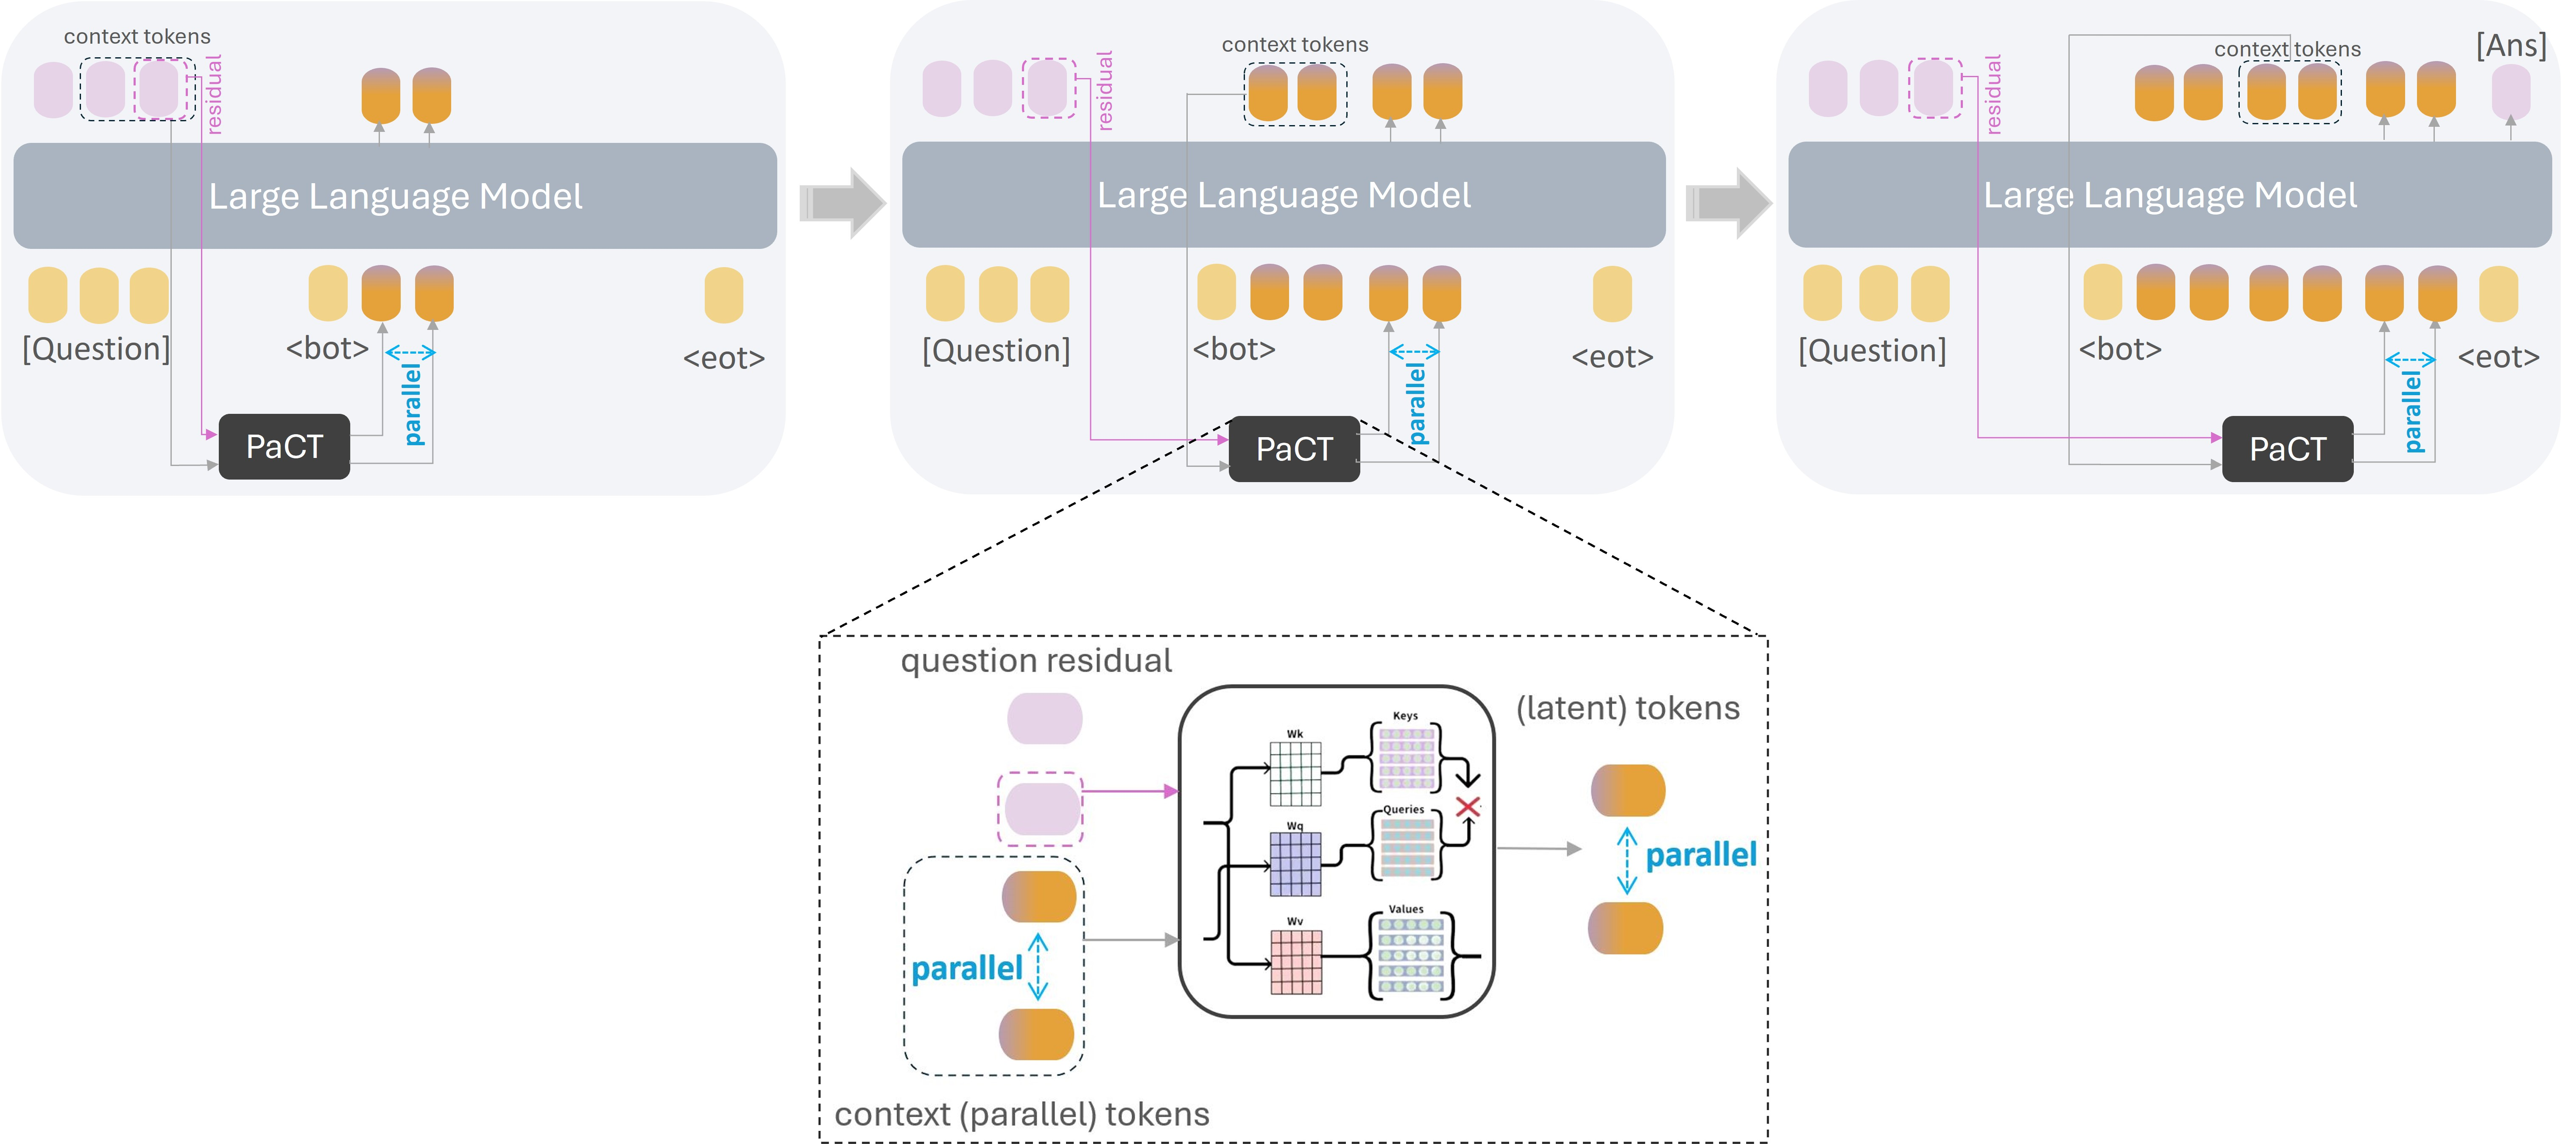
\includegraphics[width=\linewidth]{imgs/parallel_thinking_in_PaCT.jpg}
%   \caption{Parallel Continuous Thought (PaCT). At each stage, a set of latent reasoning states is synthesized in parallel from the current textual context, refined through bidirectional interaction, and used to condition subsequent autoregressive decoding.}
%   \label{fig:pact_overview}
% \end{figure*}

% PaCT replaces recurrent latent unrolling with \emph{stage-wise parallel latent reasoning}. Each stage
% constructs multiple latent reasoning states simultaneously from the current textual context, refines
% them through structured interaction, and exposes them to subsequent token decoding. Conceptually, a
% single PaCT stage proceeds as follows:

% \begin{center}
% \begin{tikzpicture}[
%     node/.style={
%         draw,
%         rounded corners,
%         inner sep=2pt,
%         font=\scriptsize
%     },
%     arrow/.style={->, thick}
% ]
% \node[node] (e) {\textbf{Text Encoding}};
% \node[node, right=4mm of e] (s) {\textbf{Latent Synthesis}};
% \node[node, right=4mm of s] (d) {\textbf{Latent Refinement}};
% \node[node, right=4mm of d] (c) {\textbf{Decoding}};

% \draw[arrow] (e) -- (s);
% \draw[arrow] (s) -- (d);
% \draw[arrow] (d) -- (c);

% \node[below=1mm of e, font=\small] {Causal};
% \node[below=1mm of s, font=\small] {Parallel};
% \node[below=1mm of d, font=\small] {Bidirectional};
% \node[below=1mm of c, font=\small] {Causal};
% \end{tikzpicture}
% \end{center}

% This structure preserves causal text processing and decoding, while enabling parallel computation
% and bidirectional interaction within each latent reasoning stage.

% \subsubsection{Latent capacity via learnable query slots}
% \label{sec:codebook}

% Let $L$ denote the number of latent reasoning states per reasoning stage. PaCT maintains a learnable set of
% query vectors
% \[
% Q = \{q_1,\dots,q_L\}, \qquad q_i \in \mathbb{R}^d,
% \]
% which define the \emph{width} of the latent reasoning set. These queries persist across examples and
% extract task-relevant summaries from the current textual context.

% \subsubsection{Parallel latent synthesis}
% \label{sec:latent_synthesis}

% Given the hidden states $H \in \mathbb{R}^{T \times d}$ of the current text prefix, PaCT synthesizes all
% latent reasoning tokens within a stage in a single cross-attention operation:
% \[
% Z = \mathrm{CrossAttn}(Q, K, V), \qquad K = V = H.
% \]
% This produces $Z \in \mathbb{R}^{L \times d}$ \emph{in parallel}. Unlike Coconut, the number of latent
% states is no longer tied to the number of sequential Transformer invocations.

% \subsubsection{Latent refinement through bidirectional interaction}
% \label{sec:latent_refinement}

% After synthesis, the latent reasoning states interact through latent-only self-attention with a
% bidirectional mask:
% \[
% Z' = \mathrm{SelfAttn}(Z).
% \]
% This interaction is confined for laten tokens within each reasoning states and does not violate causality, as
% latents do not attend to future answer tokens. Bidirectional interaction enables coordination among
% latent hypotheses within a stage, while each stage remains causally conditioned on the current text.
% Further implementation details and stability considerations are provided in Appendix~\ref{app:stability}.

% \begin{figure}[h]
%   \centering
%   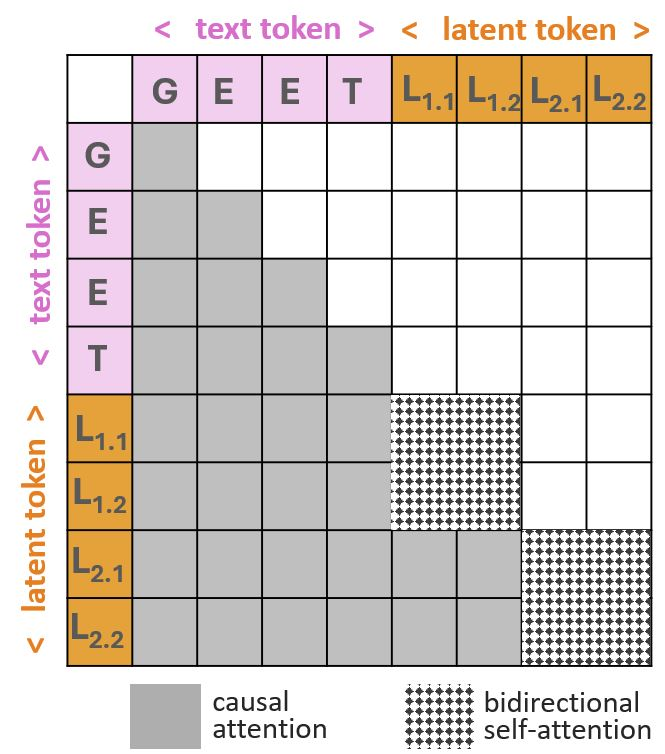
\includegraphics[width=0.6\linewidth]{imgs/bidirectional_self_attention.JPG}
%   \caption{Bidirectional interaction among latent reasoning states within a stage, while preserving causal text decoding.}
%   \label{fig:latent_attention}
% \end{figure}

% \subsubsection{Conditioning decoding on latents}
% \label{sec:conditioning}

% Autoregressive decoding is conditioned on the latent reasoning states through a causal interface:
% answer tokens may attend to both prior text tokens and all latent states produced in previous stages.
% We implement this by concatenating latent states into the attention context and adding a cross-attention
% pathway from text representations to latent keys and values. The resulting factorization is
% \[
% p(a \mid q) \;\approx\; p(a \mid q,\; Z'^{(1:S)}),
% \]
% where $Z'^{(1:S)}$ denotes the continuous latent reasoning tokens across $S$ stages. The precise attention masking
% rules are given in Appendix~\ref{app:masking}.

% \subsubsection{Multi-stage latent reasoning}
% \label{sec:stages}

% PaCT applies the above procedure for $S$ stages, yielding two scaling axes: width $L$ (latent states
% per stage) and depth $S$ (number of stages). Increasing depth introduces additional reasoning steps
% without increasing latent width or serial dependency. Empirically, we find that scaling depth is more
% effective than scaling width, consistent with latent similarity analyses presented later.

% \subsection{Training}
% \label{sec:training}

% PaCT is trained using a curriculum similar to Coconut~\cite{hao2024training}, which progressively
% replaces supervised text CoT tokens with continuous latent states. At curriculum stage $s$, the first
% $m_s$ rationale tokens are replaced by $S_s$ latent stages, while the remaining rationale (if any)
% and the answer remain as language tokens.

% Training minimizes the standard next-token prediction loss on text tokens, with the loss masked on
% latent positions:
% \[
% \mathcal{L}(\theta) = -\sum_{t \in \mathcal{I}_{\text{text}}}
% \log p_\theta(x_t \mid x_{<t}, Z'^{(1:S)}).
% \]
% The full training algorithm is provided in Appendix~\ref{app:algorithm}.

% \subsection{Computational analysis}
% \label{sec:complexity}

% Efficiency is governed by serial depth, i.e., the length of the critical path that cannot be
% parallelized. Let $T$ be the number of text decoding steps and $n_{\text{lat}}$ the total number of
% latent states.

% In Coconut, latent states are generated recurrently, yielding
% \[
% D_{\text{seq}}^{\textsc{Coconut}} = T + n_{\text{lat}}.
% \]
% In PaCT, $L$ latent states are generated in parallel per stage, and only the number of stages $S$
% contributes to serial depth:
% \[
% D_{\text{seq}}^{\textsc{PaCT}} = T + S, \qquad n_{\text{lat}} = S L.
% \]
% Thus, for a fixed latent budget, PaCT reduces latent-induced serial depth by a factor of $L$. PaCT
% shifts computation from serialized Transformer invocations to parallel attention and matrix
% multiplications, enabling substantially improved hardware utilization.
\section{Methodology}
\label{sec:method}

\subsection{Objective and problem formulation}
\label{sec:objective}

We study supervised reasoning tasks where each training example consists of a question $q$,
an optional chain-of-thought expressed as text tokens $r = (r_1,\dots,r_M)$, and a final answer
$a = (a_1,\dots,a_N)$. The full textual sequence is
\[
y \;=\; [\,q \,;\, r \,;\, a\,].
\]
A standard causal language model (LM) parameterized by $\theta$ learns $p_\theta(y)$ via maximum
likelihood training.

\paragraph{Goal.}
Our goal is to enable multi-step reasoning using \emph{continuous} internal representations while
preserving standard autoregressive decoding of the answer, and crucially, avoiding the \emph{serial}
compute bottleneck that arises when continuous reasoning is implemented through recurrent latent
unrolling.
\vspace{-3mm}
\paragraph{Key bottleneck.}
% Chain of Continuous Thought (Coconut)~\cite{hao2024training} replaces segments of textual chain-of-thought
% (CoT) tokens with continuous latent states, but generates these latent states \emph{sequentially} by
% feeding the previous hidden state back as the next input embedding. This induces a recurrent dependency
% across latent steps, causing serial depth to grow linearly with the number of latent states and limiting
% hardware parallelism. Moreover, each latent state must implicitly carry forward information from
% earlier steps, reducing representational separation across reasoning stages.
Chain of Continuous Thought (Coconut)~\cite{hao2024training} replaces segments of textual chain-of-thought
(CoT) tokens with continuous latent states, but generates these states \emph{sequentially} by feeding the
previous hidden state back as the next input embedding. This induces recurrent dependencies across latent
steps, causing serial depth to grow linearly with the number of latent states, limiting hardware
parallelism, and reducing representational separation across reasoning stages.

\vspace{-3mm}

\paragraph{Hypothesis.}
We hypothesize that the benefits of continuous latent reasoning do not require recurrent latent
unrolling. Instead, effective reasoning can be achieved by (i) synthesizing a \emph{set} of latent
reasoning states in parallel from the current textual context, (ii) allowing structured interaction
\emph{within} each reasoning stage, and (iii) conditioning autoregressive decoding on these states
through a causal interface, without directly propagating latent states across stages.

\subsection{Preliminaries: causal LMs and Coconut-style latent replacement}
\label{sec:prelims}

A causal Transformer LM maps token prefixes $x_{\le t}$ to hidden states
$H_t \in \mathbb{R}^{t \times d}$ and predicts the next token via
\[
p_\theta(x_{t+1}\mid x_{\le t}) = \mathrm{softmax}(W h_t).
\]

Coconut~\cite{hao2024training} replaces a prefix of textual CoT tokens with continuous latent states
that are not decoded as language. During this latent phase, each latent state is generated by feeding
the previous hidden state as the next input embedding, creating a recurrent unrolling within the
Transformer, reinstating an RNN-like bottleneck within an otherwise parallel architecture.

\subsection{Parallel Continuous Thought (PaCT)}
\label{sec:pact}

\begin{figure*}[t]
  \centering
  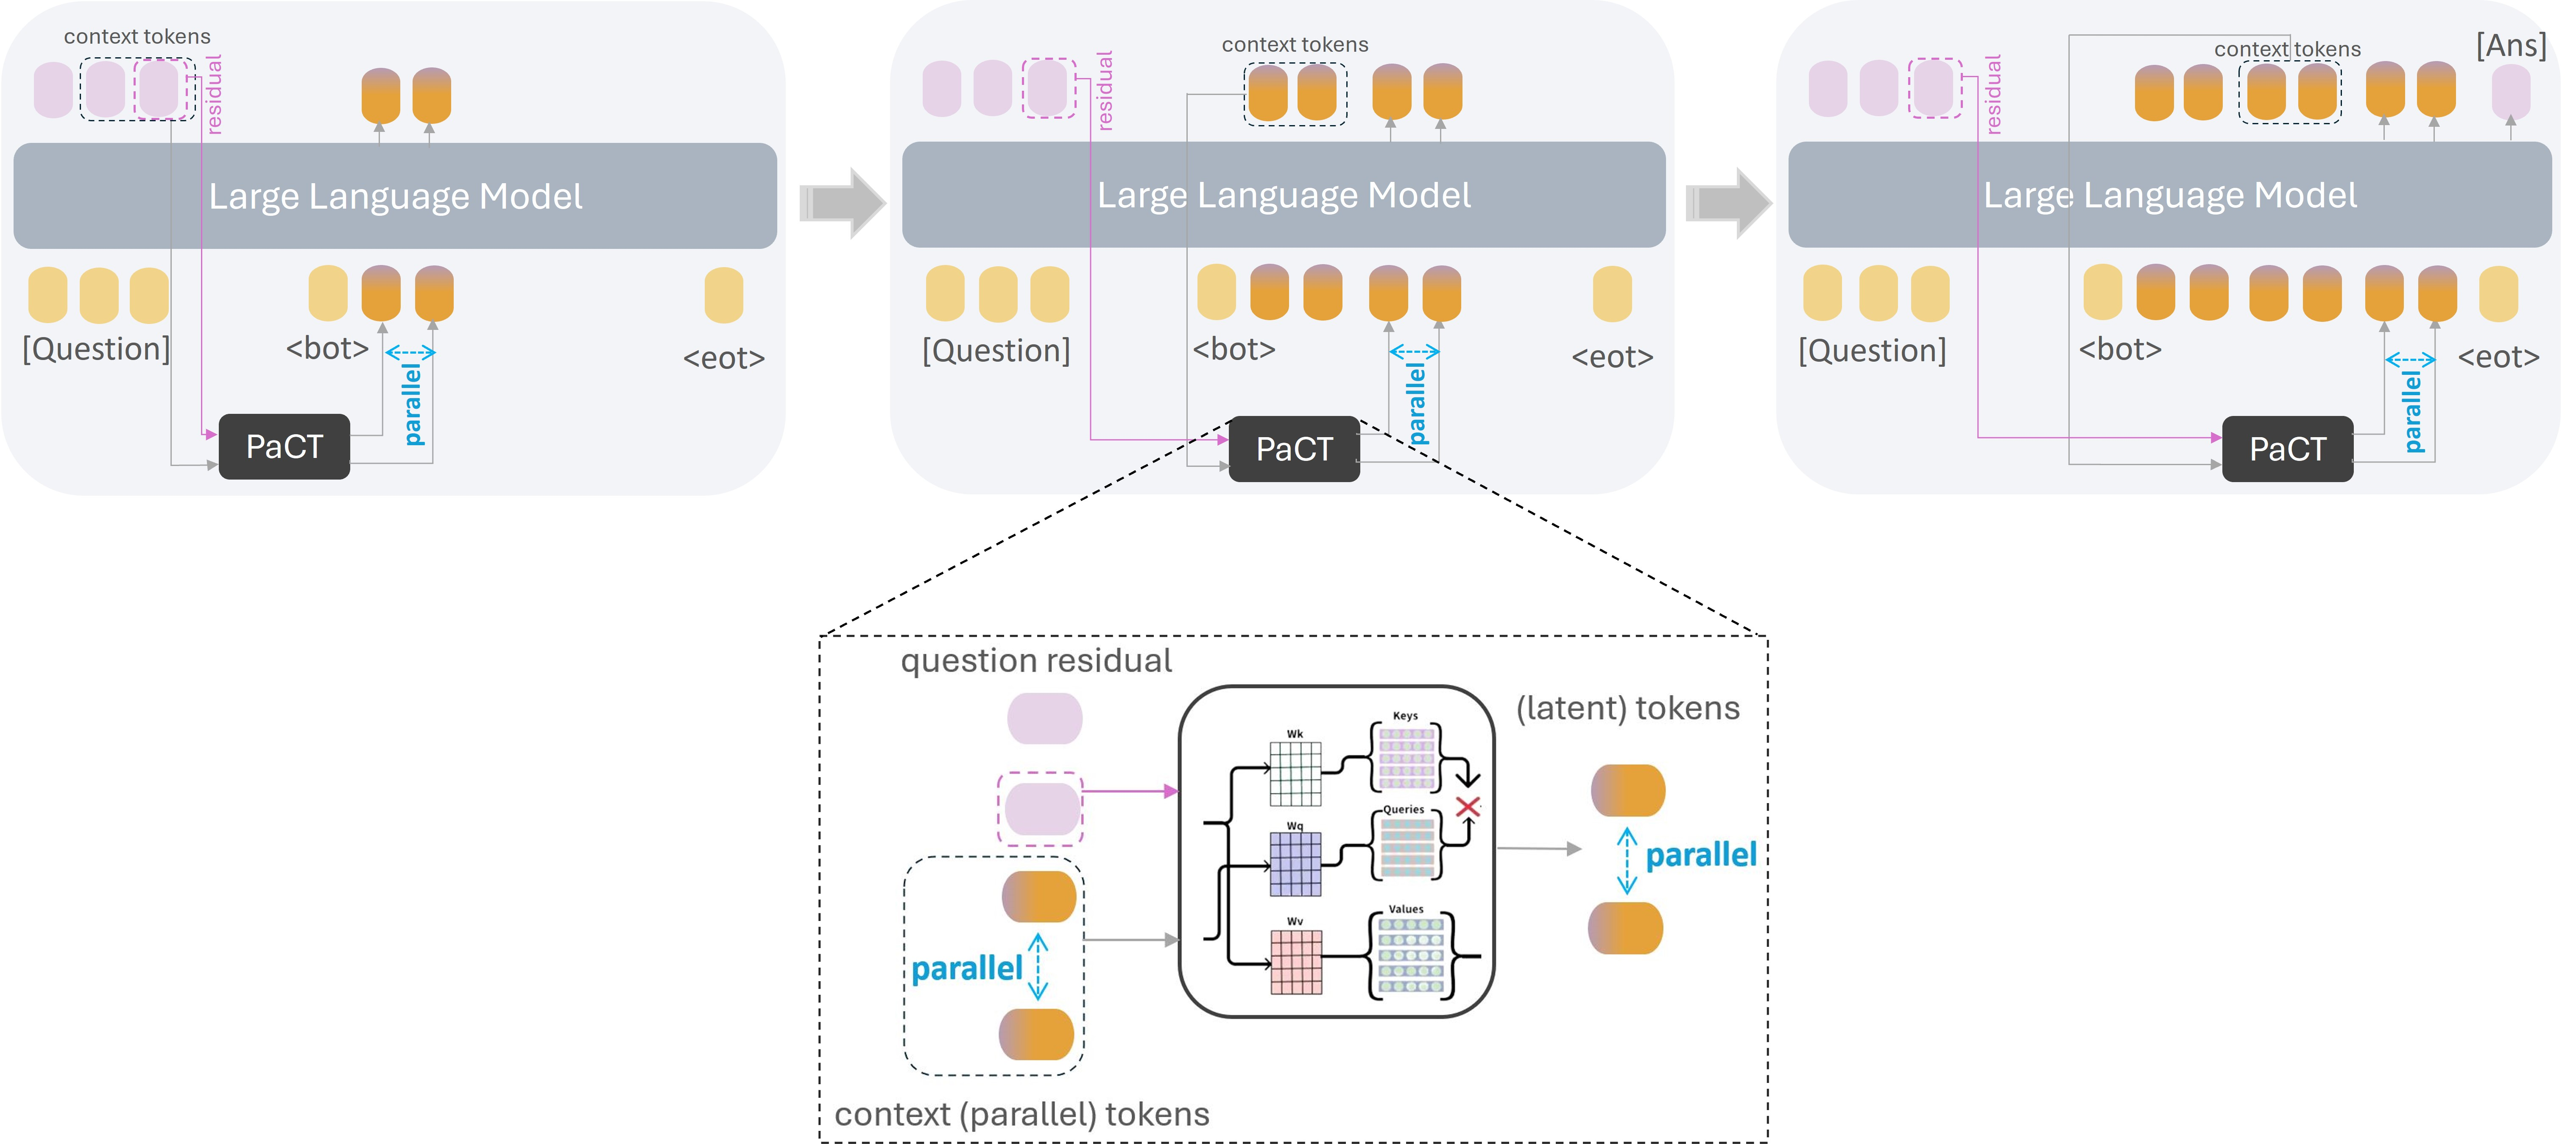
\includegraphics[width=0.9\linewidth]{imgs/parallel_thinking_in_PaCT.jpg}
  \caption{\textbf{Parallel Continuous Thought (PaCT).} At each reasoning stage, a set of latent reasoning states
  is synthesized in parallel from the current textual context, refined through bidirectional interaction,
  and used to condition subsequent autoregressive decoding.}
  \label{fig:pact_overview}
\end{figure*}

PaCT replaces recurrent latent unrolling with \emph{stage-wise parallel latent reasoning}. Rather than
propagating latent states across time, PaCT organizes reasoning into a sequence of stages. Each stage
constructs a fresh set of latent reasoning states directly from the current textual context, allows
structured interaction among them, and then exposes them to subsequent decoding. Importantly, latent
states do not directly transform or depend on latent states from earlier stages. Parallelism in PaCT arises as a consequence of stage-wise latent resynthesis: since latent reasoning states are re-synthesized from the current context rather than propagated from previous states, they can be generated simultaneously within each stage.

Conceptually, a single PaCT reasoning stage proceeds as follows:

\begin{center}
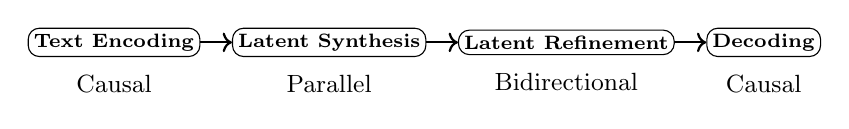
\begin{tikzpicture}[
    node/.style={
        draw,
        rounded corners,
        inner sep=2pt,
        font=\scriptsize
    },
    arrow/.style={->, thick}
]
\node[node] (e) {\textbf{Text Encoding}};
\node[node, right=4mm of e] (s) {\textbf{Latent Synthesis}};
\node[node, right=4mm of s] (d) {\textbf{Latent Refinement}};
\node[node, right=4mm of d] (c) {\textbf{Decoding}};

\draw[arrow] (e) -- (s);
\draw[arrow] (s) -- (d);
\draw[arrow] (d) -- (c);

\node[below=1mm of e, font=\small] {Causal};
\node[below=1mm of s, font=\small] {Parallel};
\node[below=1mm of d, font=\small] {Bidirectional};
\node[below=1mm of c, font=\small] {Causal};
\end{tikzpicture}
\end{center}

This structure preserves causal text processing and decoding, while enabling parallel computation and
bidirectional interaction \emph{within} each reasoning stage.

\subsubsection{Latent capacity via learnable query slots}
\label{sec:codebook}

Let $L$ denote the number of latent reasoning states per stage. PaCT maintains a learnable set of query
vectors
\[
Q = \{q_1,\dots,q_L\}, \qquad q_i \in \mathbb{R}^d,
\]
which define the \emph{width} of the latent reasoning set. These queries persist across examples and
extract task-relevant summaries from the current textual context. We use the term \emph{latent reasoning
state} to denote a continuous hidden vector that participates in reasoning but is never decoded as
language.

\subsubsection{Parallel latent synthesis}
\label{sec:latent_synthesis}

Given the hidden states $H \in \mathbb{R}^{T \times d}$ of the current text prefix, PaCT synthesizes all
latent reasoning states for a stage in a single cross-attention operation:
\[
Z = \mathrm{CrossAttn}(Q, K, V), \qquad K = V = H.
\]
This produces $Z \in \mathbb{R}^{L \times d}$ \emph{in parallel}. In contrast to Coconut, the number of
latent reasoning states is no longer tied to the number of sequential Transformer invocations, and no
latent state depends on another for its construction.

\subsubsection{Latent refinement within a stage}
\label{sec:latent_refinement}

After synthesis, latent reasoning states interact \emph{only within the same stage} through latent-only
self-attention with a bidirectional mask:
\[
Z' = \mathrm{SelfAttn}(Z).
\]
This bidirectional interaction enables coordination among latent hypotheses within a stage. It does
not violate causality, as latent states do not attend to future answer tokens, and text tokens do not
attend to latent states. No bidirectional interaction occurs across different stages.

\begin{figure}[h]
  \centering
  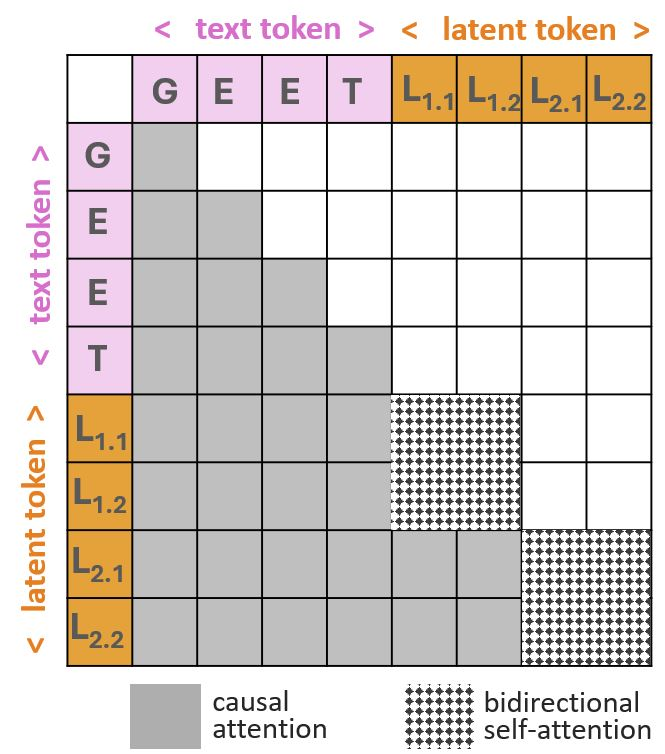
\includegraphics[width=0.4\linewidth]{imgs/bidirectional_self_attention.JPG}
  \caption{Bidirectional interaction among latent reasoning states within a single stage, while
  preserving causal text decoding.}
  \label{fig:latent_attention}
\end{figure}

\subsubsection{Conditioning decoding on latent reasoning states}
\label{sec:conditioning}

Autoregressive decoding is conditioned on latent reasoning states through a causal interface. Answer
tokens may attend to both prior text tokens and all latent reasoning states produced in \emph{earlier
stages}. Latent states themselves never attend to answer tokens.

Concretely, we concatenate latent reasoning states into the attention context and add a cross-attention
pathway from text representations to latent keys and values. This realizes the factorization
\[
p(a \mid q) \;\approx\; p(a \mid q,\; Z'^{(1:S)}),
\]
where $Z'^{(1:S)}$ denotes the latent reasoning states across $S$ stages. The attention masking rules
that enforce this causal structure are detailed in Appendix~\ref{app:masking}.

\subsubsection{Multi-stage latent reasoning}
\label{sec:stages}

PaCT applies the above procedure for $S$ reasoning stages. All latent states within a stage are synthesized
simultaneously from a restricted window of the most recent $k$ positions in the sequence, which may include
text tokens, latent states from earlier stages, or both. The window size $k$ is a fixed hyperparameter,
with its impact analyzed in Table~\ref{tab:gpt2_gsm8k_context} and Figure~\ref{fig:attention_heatmap}.
This yields two independent scaling axes: width $L$ (latent states per stage) and depth $S$ (number of
reasoning stages). Increasing depth adds reasoning capacity without increasing latent width or serial
dependency.


\subsection{Training}
\label{sec:training}

PaCT is trained using a curriculum similar to Coconut~\cite{hao2024training}, which progressively
replaces steps of CoT with continuous latent reasoning tokens. 
At curriculum stage $s$, a prefix of the textual chain-of-thought is replaced by $s$ latent reasoning stages, each consisting of $L$ latent reasoning states synthesized in parallel. The remaining CoT tokens (if any) and the answer remain as language tokens. This curriculum stabilizes optimization compared to training directly from $(q, a)$ pairs.

Training minimizes the standard next-token prediction loss on text tokens, with the loss masked on
latent positions:
\[
\mathcal{L}(\theta) = -\sum_{t \in \mathcal{I}_{\text{text}}}
\log p_\theta(x_t \mid x_{<t}, Z'^{(1:S)}).
\]
The full training algorithm is provided in Appendix~\ref{app:algorithm}.

\subsection{Computational analysis}
\label{sec:complexity}

Efficiency is governed by serial depth, i.e., the length of the critical path that cannot be
parallelized. Let $T$ be the number of text decoding steps and $n_{\text{lat}}$ the total number of
latent reasoning states.

In Coconut, latent reasoning states are generated recurrently, yielding
\[
D_{\text{seq}}^{\textsc{Coconut}} = T + n_{\text{lat}}.
\]
In PaCT, $L$ latent reasoning states are generated in parallel per stage, and only the number of
stages $S$ contributes to serial depth:
\[
D_{\text{seq}}^{\textsc{PaCT}} = T + S, \qquad n_{\text{lat}} = S L.
\]
Thus, for a fixed latent budget, PaCT reduces latent-induced serial depth by a factor of $L$. PaCT
shifts computation from the critical path to parallel attention and matrix multiplications, which
modern accelerators can efficiently amortize.


% \section{Methodology}
\label{sec:method}

\subsection{Objective and problem formulation}
\label{sec:objective}

We study supervised reasoning tasks where each training example provides a question $q$,
an optional chain-of-thought $r = (r_1,\dots,r_M)$, and a final answer
$a = (a_1,\dots,a_N)$. We write the full textual sequence as
\[
y \;=\; [\,q \,;\, r \,;\, a\,].
\]
A standard causal language model learns $p_\theta(y)$ and is trained by maximum likelihood.

\paragraph{Goal.}
We seek a model that (i) performs multi-step reasoning using \emph{continuous} internal states
rather than explicit rationale tokens, while (ii) preserving the autoregressive semantics of answer
generation, and (iii) avoiding the \emph{serial} compute overhead incurred when continuous reasoning
is designed as a recurrent unrolling.

\paragraph{Key bottleneck.}
Coconut \cite{hao2024training} demonstrates that replacing parts of the rationale with continuous hidden states can improve
reasoning quality, but it constructs continuous thoughts \emph{sequentially} by feeding the previous
hidden state back as the next input embedding, which enforces a recurrence and introduces a serial
dependence across latent steps. This makes the cost grow linearly with the number of latent steps and
limits hardware parallelism. 

\paragraph{Hypothesis.}
The central hypothesis behind proposed {Parallel Continuous Thought (PaCT)} is that the benefits of
continuous latent reasoning do not require \emph{recurrent} latent unrolling. Instead, following can be carried out 
(i) synthesize a \emph{set} of latent reasoning states in parallel from the current textual context,
(ii) allow rich interaction \emph{within} this latent workspace, and (iii) condition answer decoding on
this workspace under a causal interface. 


\subsection{Preliminaries: causal LMs and Coconut-style latent replacement}
\label{sec:prelims}

\paragraph{Causal transformer LM.}
Let $\mathcal{V}$ be the vocabulary and $d$ the hidden size. A causal LM maps token prefixes
$x_{\le t}=(x_1,\dots,x_t)$ to hidden states $H_t\in\mathbb{R}^{t\times d}$ and next-token probabilities:
\[
\begin{aligned}
H_t &= \mathrm{Transformer}_\theta\!\left(e(x_{\le t})\right), \\
p_\theta(x_{t+1}\mid x_{\le t})
&= \mathrm{softmax}(W h_t).
\end{aligned}
\]




Training minimizes the negative log-likelihood (cross-entropy) over target tokens.

\paragraph{Chain of continuous thought.}
Coconut \cite{hao2024training} replaces a prefix of rationale tokens by \emph{continuous thoughts} that are not decoded as
language. During latent mode, the input embedding at the next latent position is the previous hidden
state, creating a sequential recurrence; the LM loss is masked on latent positions. Training uses a
curriculum that progressively replaces the first $k$ rationale steps by $k\!\times\!c$ continuous thoughts.


\paragraph{Limitation.}
Each continuous thought in Coconut depends on the previous thought, producing $n$ latent
steps requires $n$ serial Transformer invocations along with decoding, which reinstates an RNN-like bottleneck inside a Transformer. 


\subsection{Parallel Continuous Thought (PaCT)}
\label{sec:pact}

\begin{figure*}[h!]
  \centering
  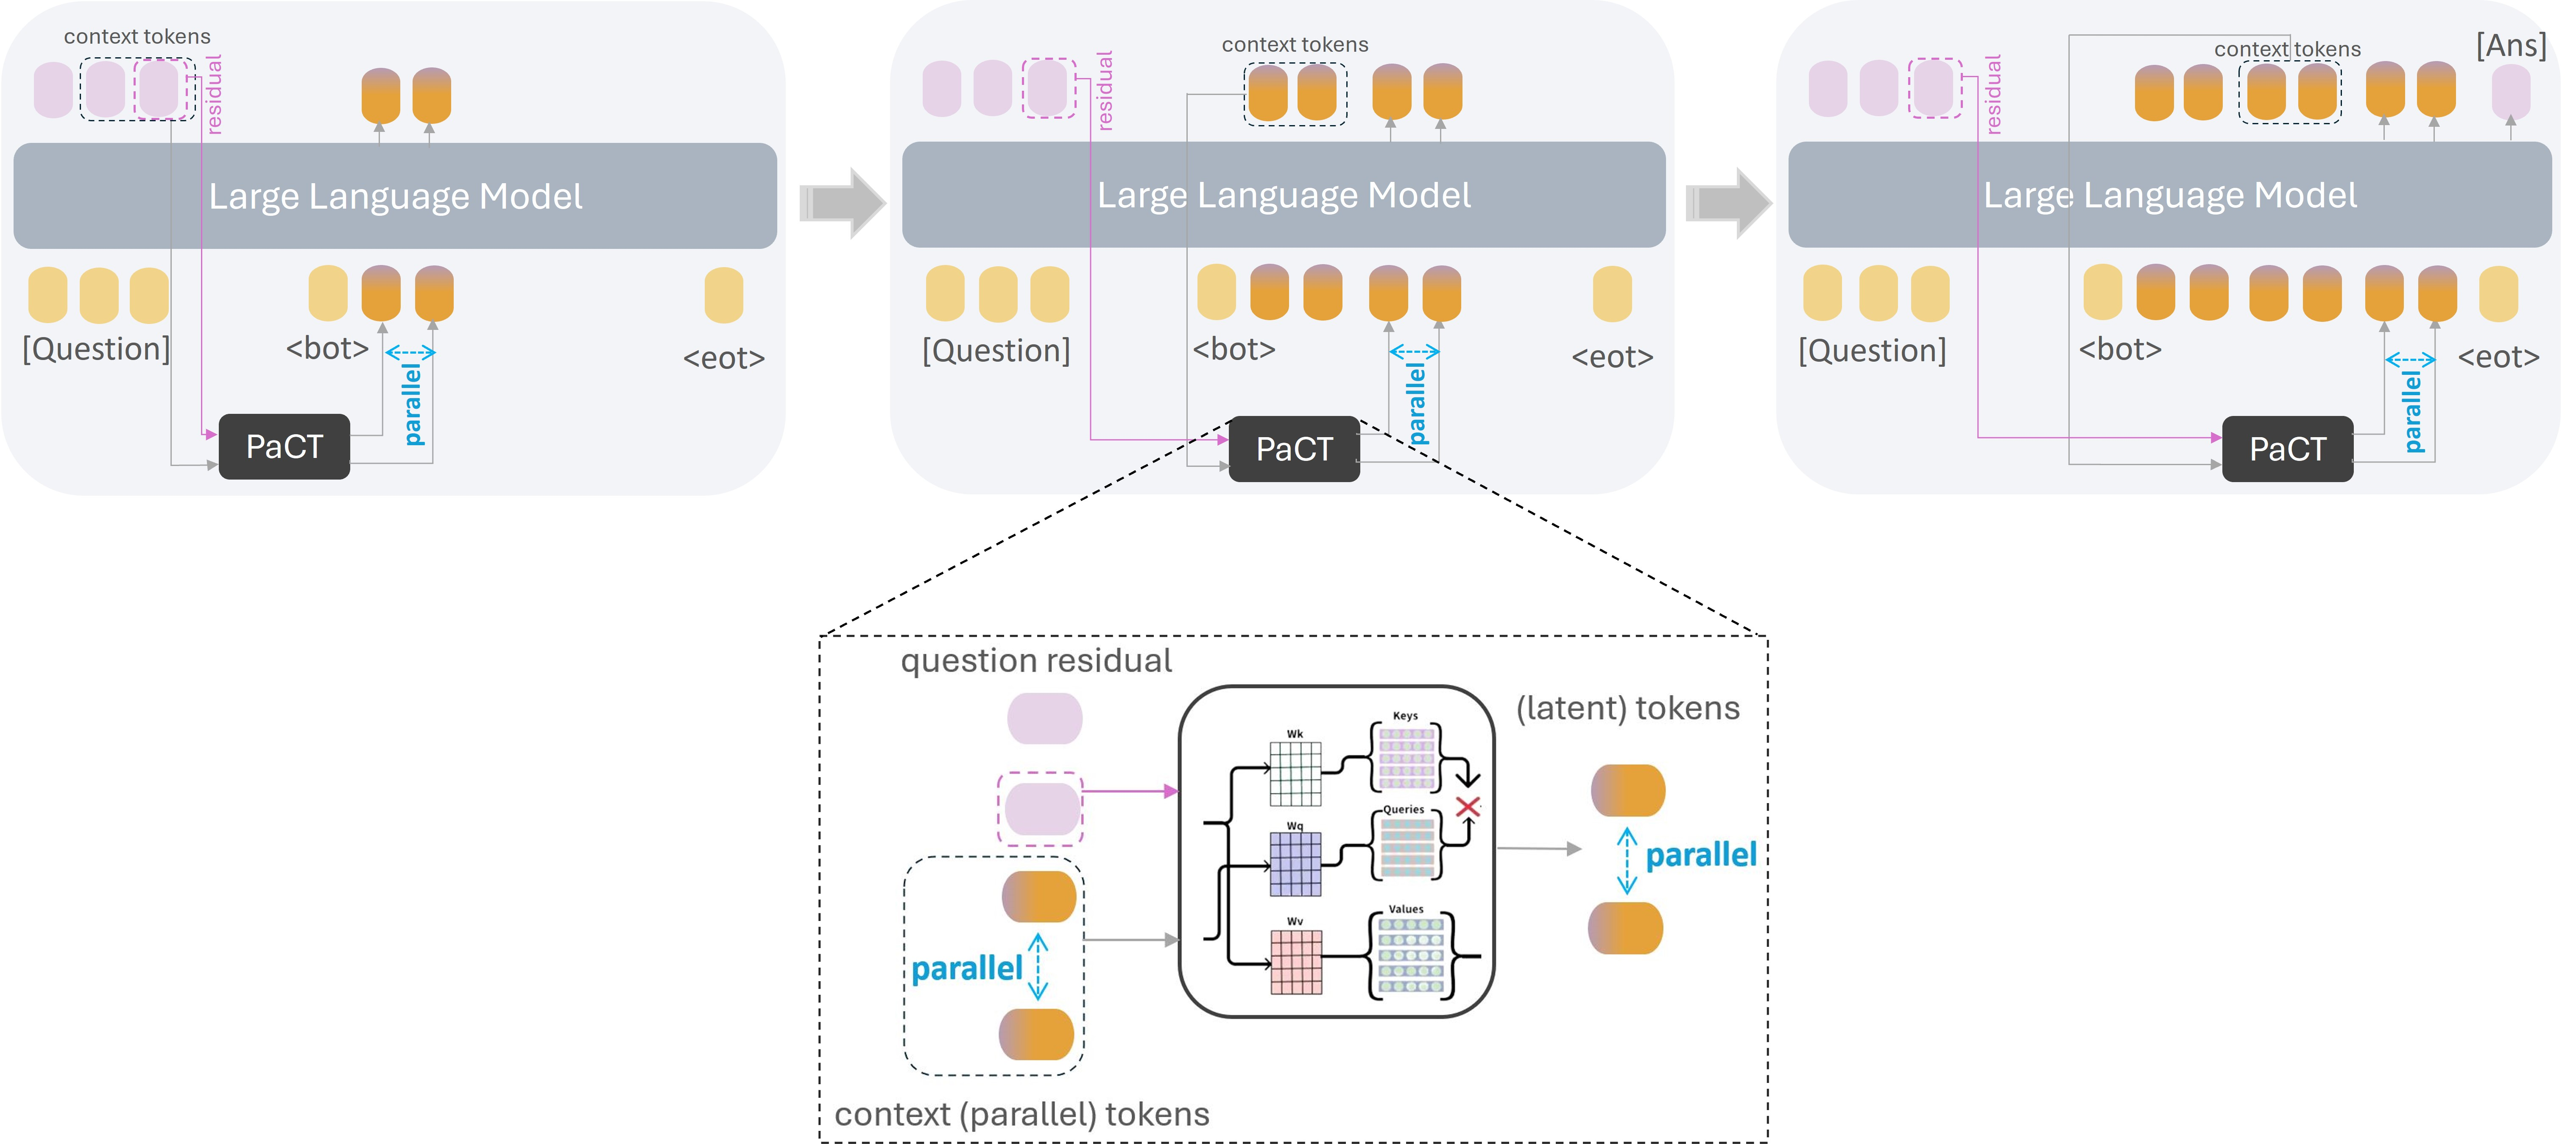
\includegraphics[width=\linewidth]{imgs/parallel_thinking_in_PaCT.jpg}
  %\vspace{2mm}
      \caption{PaCT generates latent tokens in parallel via cross-attention to the textual context, with bidirectional interaction in the latent space}
  \label{fig:PaCT_module}
\end{figure*}

PaCT replaces recurrent latent unrolling with a \emph{parallel latent workspace} updated in
\emph{stages}. Each stage constructs multiple latent vectors simultaneously, refines them via
bidirectional latent interaction, and then exposes them to subsequent token decoding.
Conceptually, one stage performs:

\begin{center}
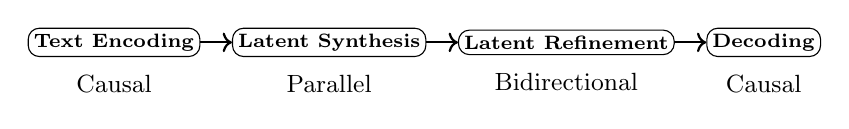
\begin{tikzpicture}[
    node/.style={
        draw,
        rounded corners,
        inner sep=2pt,
        font=\scriptsize
    },
    arrow/.style={->, thick}
]
\node[node] (e) {\textbf{Text Encoding}};
\node[node, right=4mm of e] (s) {\textbf{Latent Synthesis}};
\node[node, right=4mm of s] (d) {\textbf{Latent Refinement}};
\node[node, right=4mm of d] (c) {\textbf{Decoding}};

\draw[arrow] (e) -- (s);
\draw[arrow] (s) -- (d);
\draw[arrow] (d) -- (c);

\node[below=1mm of e, font=\small] {Causal};
\node[below=1mm of s, font=\small] {Parallel};
\node[below=1mm of d, font=\small] {Bidirectional};
\node[below=1mm of c, font=\small] {Causal};
\end{tikzpicture}
\end{center}




This preserves autoregressive decoding while enabling parallel computation within the latent space.



\subsubsection{Latent capacity: a learnable codebook of query slots}
\label{sec:codebook}
% \begin{figure*}[h!]
%   \centering
%   \includegraphics[width=0.8\linewidth]{imgs/PaCT_module.PNG}
%   \caption{(a) Learnable codebook queries generate latent tokens in parallel via cross-attention to the textual context, with bidirectional interaction in the latent workspace; (b) the attention structure enforces causal text attention while allowing latents to attend to text and earlier latent stages, preserving autoregressive decoding. \textcolor{red}{Prakash, Incorporate suggestions from Prof.}}
%   \label{fig:PaCT_module}
% \end{figure*}


Let $L$ be the number of latent ``slots'' per stage. PaCT maintains a learnable codebook
\[
Q \;=\; \{q_1,\dots,q_L\}, \qquad q_i\in\mathbb{R}^d,
\]
which acts as a persistent set of queries that extract task-relevant summaries from the current
textual state. The codebook defines the \emph{width} of the latent workspace. 

\paragraph{Grounded initialization for stability.}
To anchor the latent workspace to the task specification, we use the question representation as a
shared residual. Let $h_q\in\mathbb{R}^d$ denote the hidden state of the final question token.
We initialize the output projection of the latent synthesis cross-attention to zero and add $h_q$ to
each latent slot after synthesis, so that at initialization all latents start as grounded copies of the
question representation and only deviate when learning discovers useful refinements. 


\subsubsection{Parallel latent synthesis by cross-attention}
\label{sec:latent_synthesis}

Let $H\in\mathbb{R}^{T\times d}$ be the hidden states of the current text prefix (question plus any
remaining rationale tokens). We synthesize latents in one operation using cross-attention with
codebook queries and contextual keys/values.

\paragraph{Context window (causal consistency).}
We optionally restrict keys/values to a recent window $H_{t-k:t}=[h_{t-k},\dots,h_t]$ to enforce that
latent updates depend only on available past information. 

\paragraph{Operator form.}
Denote standard multi-head attention by $\mathrm{Attn}(\cdot)$. Latents are produced as
\[
Z \;=\; \mathrm{CrossAttn}(Q,\;K,\;V), \qquad
K=V=H_{t-k:t},
\]
yielding $Z\in\mathbb{R}^{L\times d}$ computed \emph{in parallel}. This is the first key departure from
Coconut: the number of latent vectors is no longer tied to the number of Transformer invocations.



\subsubsection{Latent refinement via bidirectional self-attention}
\label{sec:latent_deliberation}

\begin{figure}[h]
  \centering
  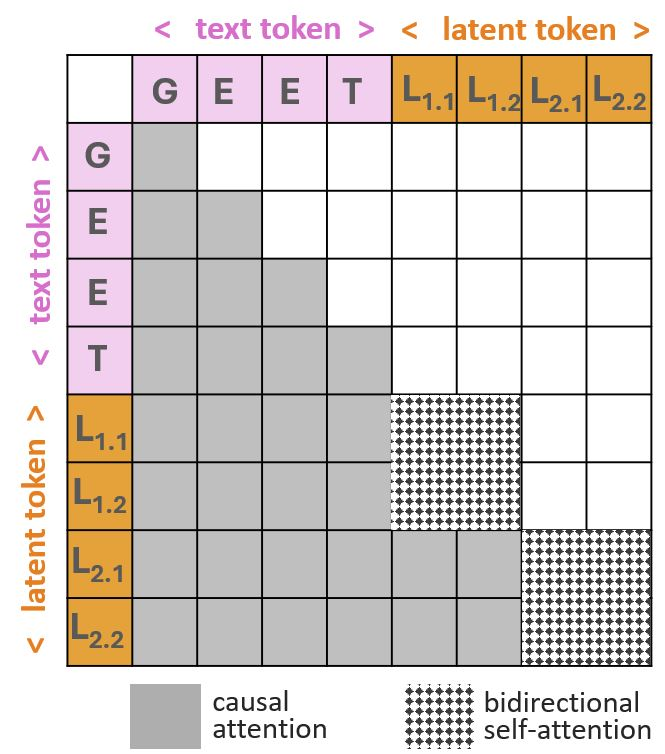
\includegraphics[width=0.6\linewidth]{imgs/bidirectional_self_attention.JPG}
  \caption{Visualizing bi-directional self-attention for latent tokens}
  \label{fig:bidirectional_self_attention}
\end{figure}

After synthesis, the latent slots refine one another within a latent-only workspace. We first ground
each latent by adding the shared question residual:
\[
\tilde{Z} \;=\; Z + \mathbf{1} h_q^\top,
\]
where $\mathbf{1}\in\mathbb{R}^L$ is the all-ones vector. We then apply latent self-attention with a
\emph{bidirectional} mask:
\[
Z' \;=\; \mathrm{SelfAttn}(\tilde{Z}).
\]
Bidirectional interaction is confined to the latent workspace: latents do not attend to future answer tokens, and earlier question tokens do not attend to latents (by causality), ensuring no label leakage while allowing rich coordination among latent hypotheses (Fig. \ref{fig:bidirectional_self_attention}). 
This residual grounding serves two purposes. First, it anchors all latent reasoning vectors to a shared semantic representation of the task specification, ensuring that deliberation remains explicitly conditioned on the question throughout the reasoning process. Second, it bounds the latent update to depend only on the current textual state, rather than the full history of latent computations, thereby reinforcing a Markovian structure in latent reasoning. Each iteration updates the latent state as a function of the current context and a fixed task representation, rather than recursively accumulating unstructured latent history.
%This workspace can be viewed as parallel hypothesis refinement: each slot receives a contextual summary, then exchanges information with other slots before conditioning decoding.


\subsubsection{Conditioning decoding on latents}
\label{sec:conditioning}

We condition subsequent decoding on the latent workspace using a causal interface:
answer tokens may attend to both prior text tokens and the latent slots produced by PaCT.
Concretely, we implement this by \textit{concatenating} latent tokens into the attention context and
adding a \textit{cross-attention pathway} from text representations to latent keys/values.
This matches the intended computation:
\[
p(a \mid q) \;\approx\; p(a \mid q,\; Z'^{(1:S)}),
\]
where $Z'^{(1:S)}$ denotes the latent workspaces across $S$ stages.



\paragraph{Causal mask.}
Let the full sequence ordering be \texttt{[question ; latent stages ; remaining text/answer]}.
We use an attention mask that enforces:
(i) text-to-text remains causal,
(ii) text cannot attend to later latents,
(iii) latents can attend to all previous text and to all latents within their stage bidirectionally,
(iv) answer tokens can attend to all earlier text and all latents.
This realizes the \textit{Text $\rightarrow$ Latents $\rightarrow$ Text} pattern while preserving autoregressive
answer generation. 


\subsubsection{Multi-stage latent reasoning (depth)}
\label{sec:stages}

We repeat the latent workspace construction for $S$ stages, where each stage produces a workspace that conditions subsequent computation. This yields two scaling axes: width $L$ (parallel slots per stage) and depth $S$ (sequential workspace updates). Empirically, increasing depth is more effective than increasing width, consistent with our latent similarity analyses showing redundancy within stages but substantial variation across stages.




\subsection{PaCT training}
\label{sec:training}

\subsubsection{Curriculum schedule}
\label{sec:curriculum}

Like Coconut, we use a curriculum that progressively removes supervised text CoT tokens and
replaces them with latent computation, which stabilizes optimization compared to training purely
from $(q,a)$ pairs. 

Let $m_s$ be the number of rationale steps replaced at curriculum stage $s$.
We construct a training sequence by replacing the first $m_s$ rationale steps with $S_s$ latent stages
(each producing $L$ latent slots). The remaining suffix rationale (if any) and the answer remain as
language tokens for supervision.

\subsubsection{Masked language modeling objective}
\label{sec:loss}

Let $\mathcal{I}_{\text{text}}$ denote indices of \emph{language} tokens (question, remaining rationale,
answer), and let $\mathcal{I}_{\text{lat}}$ denote indices occupied by latent slots. We train by minimizing
\[
\mathcal{L}(\theta) \;=\;
-\sum_{t\in \mathcal{I}_{\text{text}}}
\log p_\theta(x_{t}\mid x_{<t}, Z'^{(1:S)}),
\]
i.e., standard next-token prediction on text tokens, with the loss \emph{masked} on latent positions.
This keeps the learning signal identical in form to standard LM training while allowing latent
computation to be learned implicitly through its effect on answer likelihood. 


% \subsubsection{Algorithm}
% \label{sec:algorithm}
\begin{algorithm}[t]
\caption{Curriculum training for PaCT}
\label{alg:cct_formal}
\begin{algorithmic}[1]
\Require Dataset $\mathcal{D}$, curriculum schedule $\{m_s,S_s\}_{s=0}^{S_{\max}}$, slots $L$, parameters $\theta$, stepsize $\eta$
\For{$s=0,\dots,S_{\max}$}
  \For{$(q,r,a)\sim \mathcal{D}$}
    \State $(\tilde{r}_s,\,\mathcal{M}_s)\leftarrow \mathrm{Replace}(r;\,m_s, S_s, L)$
    \State $x_s \leftarrow [\,q;\ \tilde{r}_s;\ a\,]$
    \State $(\mathbf{p}_\theta(\cdot\mid x_s),\,Z'^{(1:S_s)}) \leftarrow \mathrm{PaCT}_\theta(x_s;\mathcal{M}_s)$
    \State $\mathcal{L}_s(\theta)\leftarrow -\sum\limits_{t\in \mathcal{I}_{\text{text}}(x_s)} \log \mathbf{p}_\theta(x_s[t]\mid x_s[<t],Z'^{(1:S_s)})$
    \State $\theta \leftarrow \theta - \eta \nabla_\theta \mathcal{L}_s(\theta)$
  \EndFor
\EndFor
\end{algorithmic}
\end{algorithm}


\subsection{Computational analysis: removing recurrent latent unrolling}
\label{sec:complexity}

Efficiency is governed by \emph{serial depth} (critical-path length), since parallel hardware can amortize
large matrix multiplications but cannot parallelize a long chain of dependent Transformer invocations.
Let $T$ be the number of causal text decoding steps (tokens for which logits are produced) and
$n_{\text{lat}}$ the number of latent reasoning vectors.

\paragraph{Serial depth.}
In Coconut, latent vectors are generated recurrently ($z_{j+1}$ depends on $z_j$), hence each latent requires
an additional dependent Transformer update:
\[
D_{\text{seq}}^{\textsc{Coconut}} = T + n_{\text{lat}}.
\]
In PaCT, latents are produced in \emph{parallel} within each stage: $L$ latent slots are synthesized by a single
codebook$\rightarrow$text cross-attention and refined by latent-only self-attention. With $S$ stages and
$n_{\text{lat}}=SL$,
\[
D_{\text{seq}}^{\textsc{PaCT}} = T + S,
\qquad\text{so}\qquad
\frac{D_{\text{seq}}^{\textsc{Coconut}}-T}{D_{\text{seq}}^{\textsc{PaCT}}-T}=\frac{n_{\text{lat}}}{S}=L.
\]
Thus, for a fixed latent budget $n_{\text{lat}}$, PaCT reduces the latent-induced serial depth by a factor of $L$.

PaCT shifts computation from a serialized chain to parallel attention/GEMM operations:
per stage, cross-attention over a context window of length $k$ costs $\tilde{O}(Lkd)$ and latent self-attention costs
$\tilde{O}(L^2d)$. Increasing width $L$ therefore increases \emph{parallel work} but does not increase the critical path;
only increasing the number of stages $S$ increases serial depth. This width--depth decoupling is the core computational
advantage of PaCT over recurrent latent unrolling.

%%%%%%%%


%%%%%%%%


%%%%%%%%%%%%
%%%%%%%%%%%%%%%%%%%%%%%%%%%%%%%%%%%%%%%%%%%%%%%%%%%%%%%%%%%%%%%%%%%%%%%
\section{Results and Discussion}
\label{sec:results}

\paragraph{Results overview.}
PaCT removes the recurrent latent-unrolling bottleneck while preserving (and often improving) reasoning performance.
Across GSM8k, ProntoQA, and ProsQA, PaCT matches or exceeds Coconut while reducing training time by $3.2$--$4.7\times$
(Table~\ref{tab:main_results}), and these gains persist at larger model scales (Table~\ref{tab:performance_training}).
We then analyze \emph{why} PaCT works: (i) each latent stage contributes measurably to the final prediction
(Fig.~\ref{fig:accuracy_and_latent_stages}); (ii) PaCT promotes stage-wise specialization and scales well with depth
(Table~\ref{tab:latent_similarity}, Fig.~\ref{fig:accuracy_and_latent_stages}); (iii) latent trajectories exhibit
interpretable confidence dynamics (Table~\ref{tab:latent_confidence}, Fig.~\ref{fig:latent_examples});
and (iv) PaCT stabilizes internal dynamics relative to Coconut (Fig.~\ref{fig:icr}).
Finally, we validate a key architectural choice of restricting the cross-attention context for latent synthesis
(Sec.~\ref{subsec:context_length}).

\subsection{Experimental Setup}
\label{sec:experimental_setup}
To ensure a fair, direct comparison, we follow Coconut~\cite{hao2024training}, matching
model architectures, curriculum schedules, datasets, and optimization settings. This isolates the effect of PaCT’s
parallel latent reasoning from other confounders.
\vspace{-4mm}
\paragraph{Base models.}
Our primary experiments use GPT-2 Small (124M) as the base causal LM, without modifying the underlying Transformer
layers. To evaluate scaling with model size, we additionally run experiments using LLaMA-3B and LLaMA-8B as base
models (Table~\ref{tab:performance_training}). In all cases, PaCT is integrated on top of the base model with the
same module design.
\vspace{-4mm}
\paragraph{PaCT configuration.}
Unless stated otherwise, PaCT uses a fixed configuration: a latent query/codebook projection dimension of 128 and
4 attention heads for cross-attention. Latent synthesis uses a restricted context window consisting of the two most
recent hidden states; we ablate this choice in Sec.~\ref{subsec:context_length}.
\vspace{-4mm}
\paragraph{Curriculum training.}
We use Coconut’s multi-stage curriculum, progressively replacing textual CoT tokens with latent reasoning stages.
For GSM8k, we first fine-tune with CoT supervision for 25 epochs, followed by 25 epochs of curriculum-based latent
training. For ProntoQA and ProsQA, models are trained for 50 epochs under the same curriculum schedule as Coconut.
We set the maximum number of latent stages to 3 for GSM8k and 6 for ProntoQA and ProsQA.
\vspace{-4mm}
\paragraph{Optimization.}
We use AdamW with learning rate $1\times 10^{-4}$, weight decay 0.01, and effective batch size 128. We evaluate on
GSM8k (math), ProntoQA (deductive logic), and ProsQA (proof-oriented reasoning). Following prior work, the continuous
thought parameter is set to $c_{\text{thought}}=2$ for GSM8k and $c_{\text{thought}}=1$ for ProntoQA and ProsQA.
All experiments are conducted on a single node of H100 with four 80 GPUs.

\subsection{Parallel latent reasoning improves training efficiency without sacrificing accuracy}
\label{sec:efficiency}

\begin{table*}[t]
\centering
\begin{tabular}{lcccccc}
\toprule
\multirow{2}{*}{Method} 
& \multicolumn{2}{c}{GSM8k} 
& \multicolumn{2}{c}{ProntoQA} 
& \multicolumn{2}{c}{ProsQA} \\
\cmidrule(lr){2-3} 
\cmidrule(lr){4-5} 
\cmidrule(lr){6-7} 
& Acc. (\%) & Train Time (hrs)
& Acc. (\%) & Train Time (hrs)
& Acc. (\%) & Train Time (hrs) \\
\midrule
CoT 
& 42.90 $\pm$ 0.2 & 2.90
& 98.80 $\pm$ 0.8 & 0.55
& 77.50 $\pm$ 1.9 & 0.91 \\
No-CoT 
& 16.50 $\pm$ 0.5 & 2.18
& 93.80 $\pm$ 0.7 & 0.41
& 76.70 $\pm$ 1.0 & 0.68 \\
Pause Token 
& 16.40 $\pm$ 1.8 & 2.47
& 77.70 $\pm$ 21.0 & 0.47
& 75.90 $\pm$ 0.7 & 0.77 \\
iCoT 
& 30.00 & 2.47
& 99.80 $\pm$ 0.3 & 0.47
& 98.20 $\pm$ 0.3 & 0.77 \\
\midrule
Coconut 
& 32.00 $\pm$ 1.5 & 15.40
& 99.80 $\pm$ 0.2 & 2.11
& 97.00 $\pm$ 0.3 & 6.42 \\
CoLaR
& 26.40 $\pm$ 1.7 & 3.10
& 96.60 $\pm$ 0.6 & \textbf{0.45}
& 75.00 $\pm$ 0.8 & 6.21 \\
CODI
& 33.81 $\pm$ 1.2 & 5.90
& 78.90 $\pm$ 0.6 & 0.89
& * & * \\

\textbf{PaCT} 
& \textbf{34.40} $\pm$ 0.1 & \textbf{3.30}
& \textbf{100.0} $\pm$ 0.1 & \textit{0.65}
& \textbf{98.67} $\pm$ 0.2 & \textbf{1.58} \\
\bottomrule
\end{tabular}
\caption{\textbf{Accuracy and training efficiency across reasoning methods.}
Results are reported on GSM8k, ProntoQA, and ProsQA.
PaCT matches or exceeds Coconut across all benchmarks while substantially reducing training time.
Results for Coconut, CoLaR, and CODI are obtained by rerunning their released implementations under our experimental setup. *CODI's training was not stable on ProsQA, hence results have been ommitted.}
\label{tab:main_results}
\vspace{-7mm}
\end{table*}

Table~\ref{tab:main_results} shows that PaCT consistently reduces training time while maintaining strong reasoning
accuracy. On GSM8k, PaCT improves accuracy over Coconut (34.4 vs.\ 32.0) and reduces training time from 15.40 to
3.30 hours ($4.7\times$). On ProntoQA, PaCT matches Coconut’s accuracy (100.0 vs.\ 99.8) while reducing training time
from 2.11 to 0.65 hours ($3.2\times$). On ProsQA, PaCT improves accuracy (98.67 vs.\ 97.0) and reduces training time
from 6.42 to 1.58 hours ($4.1\times$). These gains align with the serial-depth analysis in Sec.~\ref{sec:complexity}:
PaCT removes recurrent latent unrolling and shifts latent computation to parallel attention operations within each stage. Detailed inference analysis is present in appendix \ref{sec:inference_latency}.



\subsection{Scaling to larger model sizes}
\label{sec:scaling}

\begin{table}[t]
    \centering
    \small
    \caption{\textbf{Scaling with model size.} Accuracy and training time across larger base models on GSM8k. Training time in hrs.}
    \label{tab:performance_training}
\begin{tabular}{lcccccc}
\toprule
 &  & \multicolumn{2}{c}{Coconut} & \multicolumn{2}{c}{PaCT} \\
\cmidrule(lr){3-4} \cmidrule(lr){5-6}
Model & Params & Acc & Time & Acc & Time \\
\midrule
LLaMA 3.2 & 3B & 31.7 & 51.5 & \textbf{36.4} & \textbf{11.02 (5x)} \\
LLaMA 3   & 8B & 43.6 & 105.9 & \textbf{43.6} & \textbf{22.68 (5x)} \\
\bottomrule
\end{tabular}
\vspace{-1mm}
\end{table}

Table~\ref{tab:performance_training} shows that PaCT’s efficiency gains persist at larger model scales.
On the 3B model, PaCT reduces training time from 51.5 to 11.02 hours ($4.7\times$) while improving accuracy
(31.7 $\rightarrow$ 36.4). On the 8B model, PaCT reduces training time from 105.9 to 22.68 hours ($4.7\times$)
while matching Coconut’s accuracy (43.6). This consistency supports the core claim that eliminating recurrent latent
unrolling reduces critical-path length independent of model size.

\subsection{Every latent stage contributes to performance}
\label{sec:stage_ablation}
\begin{figure}[t]
    \centering
    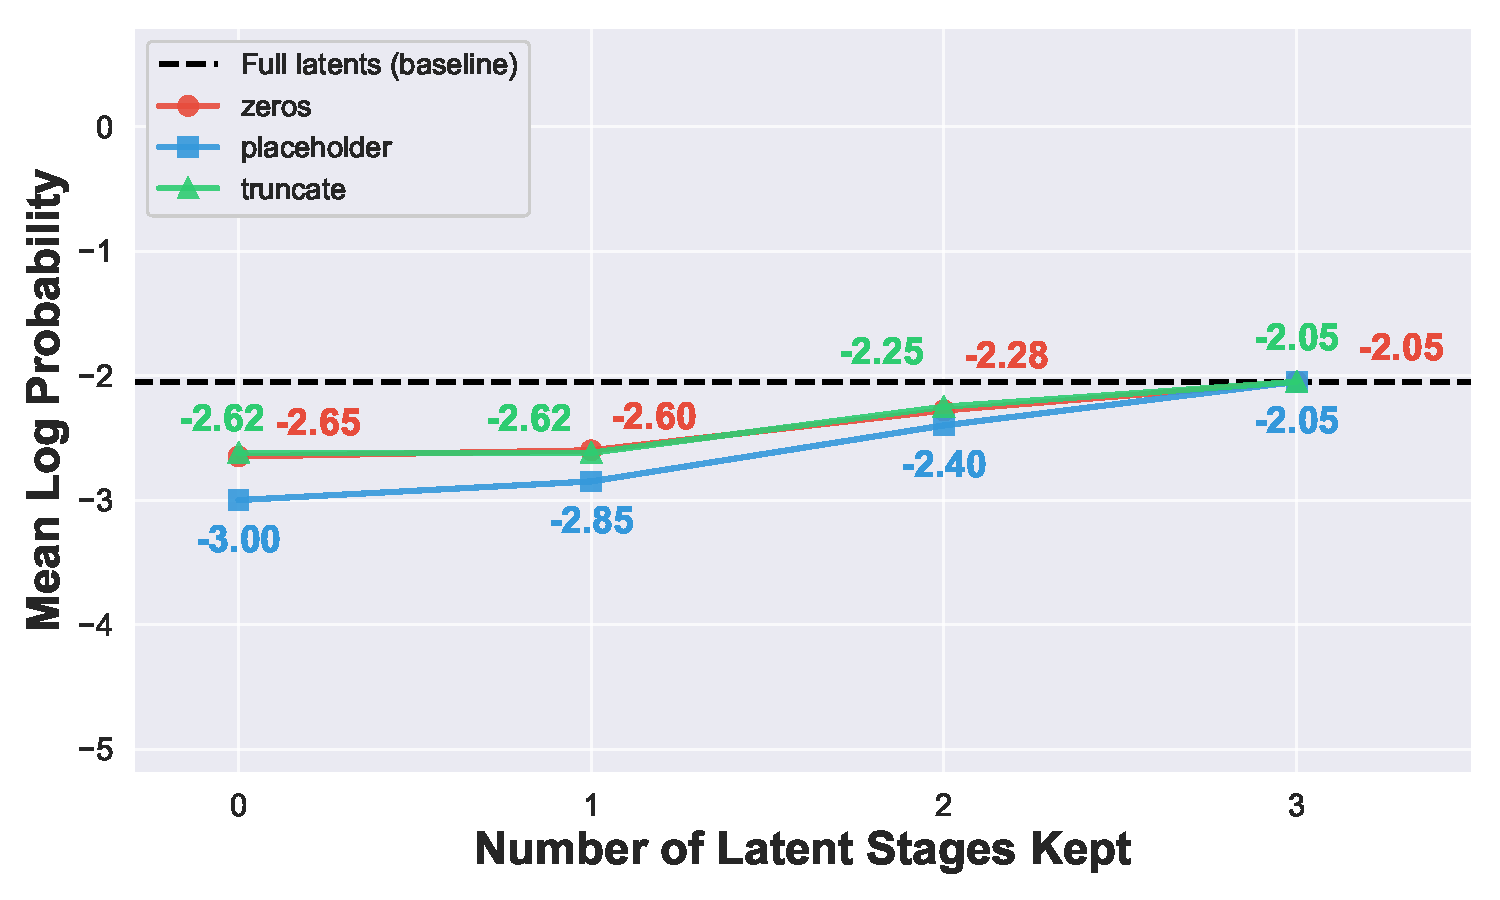
\includegraphics[width=0.49\textwidth]{imgs/ablation_log_probs_breathing_room.pdf}
    \caption{\textbf{Impact of latent stage ablation on answer confidence.} We measure the mean log-probability of ground-truth answers on GSM8k while progressively removing latent stages via zeroing, placeholder replacement, or truncation. The observed monotonic increase in probability as more stages are retained demonstrates that PaCT utilizes each computational stage to actively refine its final prediction.}
    \label{fig:latent_requirement_ablation}
    \vspace{-8mm}
\end{figure}


Efficiency gains would be unconvincing if latent stages acted as inert compute. We therefore test whether each
reasoning stage contributes to the final prediction by ablating entire stages at inference time. Concretely, we
progressively remove latent stages (each stage contains $L{=}2$ latent reasoning states on GSM8k) and measure the
resulting change in log-probability assigned to (i) the model’s generated answer token and (ii) the ground-truth
answer token.
Figure~\ref{fig:latent_requirement_ablation}
shows a clear monotonic trend: retaining more stages yields higher answer likelihood, and removing later stages causes
the largest confidence drops. This indicates that PaCT stages are actively used to refine the final prediction.

\subsection{Latent stage specialization and depth scaling}
\label{sec:latent_content}

\begin{table}[t]
\centering
\small
\caption{\textbf{Latent similarity diagnostics.} PaCT exhibits high within-stage similarity but low cross-stage similarity,
while Coconut exhibits the opposite trend.}
\label{tab:latent_similarity}
\begin{tabular}{lcc}
\toprule
Metric & PaCT & Coconut \\
\midrule
Within-stage cosine similarity & $0.99 \pm 0.01$ & $0.30 \pm 0.17$ \\
Cross-stage cosine similarity  & $0.31 \pm 0.21$ & $0.63 \pm 0.14$ \\
\bottomrule
\end{tabular}
\vspace{-6mm}
\end{table}

PaCT uses \emph{stage-wise resynthesis}: each stage constructs its latent states directly from the current textual
context and previously generated latent states, rather than recurrently transforming a single latent trajectory as in Coconut. Table~\ref{tab:latent_similarity}
offers a mechanistic view of this difference. In PaCT, latent states within the same stage are nearly identical (0.99
cosine similarity), while cross-stage similarity is much lower (0.31), suggesting that successive stages encode distinct
information. Coconut exhibits the reverse: within-stage latent states are diverse (0.30), but cross-stage similarity is
higher (0.63), consistent with recurrent unrolling that encourages information to be carried forward along a single evolving state. This structure has a direct implication: if within-stage latent states are largely redundant in PaCT, compute is better
allocated toward \emph{depth} (more stages) than toward \emph{width} (more latent states per stage), provided a
minimum of within-stage width is preserved to sustain the bidirectional refinement that makes each stage informative.
We validate this first in Figure~\ref{fig:accuracy_and_latent_stages}, which shows consistent gains from increasing
the number of stages across datasets, and then in Table~\ref{tab:width_depth_budget}, which fixes the total latent
budget and sweeps over width--depth splits.

\begin{figure}[t]
  \centering
  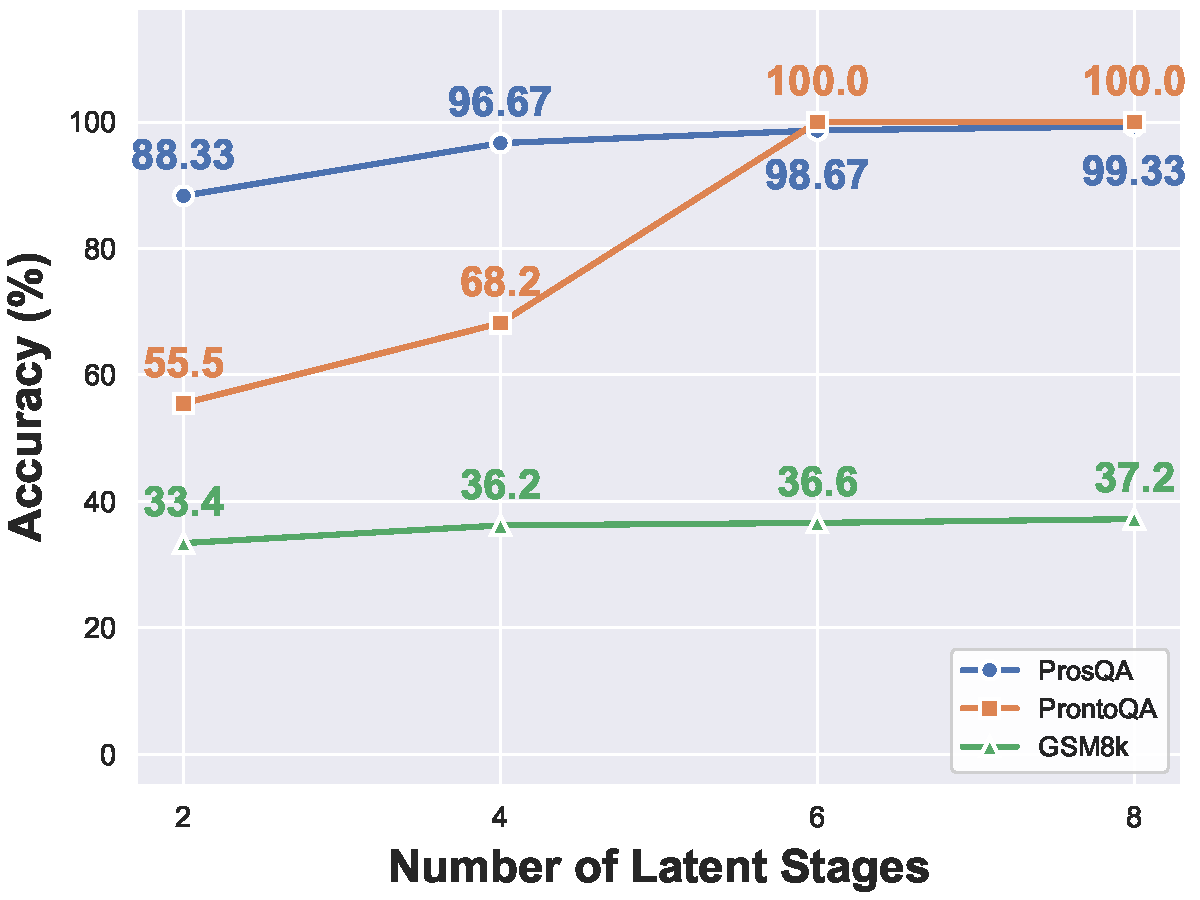
\includegraphics[width=0.8\linewidth]{imgs/table_seven_styled_values.pdf}
  \caption{\textbf{Accuracy vs.\ number of stages.} Increasing the number of latent stages improves accuracy across benchmarks.}
  \label{fig:accuracy_and_latent_stages}
\end{figure}

\paragraph{Width-depth tradeoff under a fixed latent budget.}
To disentangle the contributions of within-stage width $L$ and reasoning depth $S$, we fix the total latent budget
at $L \cdot S = 6$ on GSM8k and sweep over the four integer factorizations, keeping every other hyperparameter at
the default configuration. Table~\ref{tab:width_depth_budget} reports the resulting accuracies.

\begin{table}[t]
\centering
\small
\caption{\textbf{Width--depth allocation under a fixed latent budget.}
Holding the total number of latent reasoning states constant at $L \cdot S = 6$ on GSM8k, we vary how the budget
is split between within-stage width $L$ and reasoning depth $S$. A balanced allocation that favours depth
($L{=}2$, $S{=}3$) is best; both pure width ($S{=}1$) and pure depth ($L{=}1$) underperform.}
\label{tab:width_depth_budget}
\begin{tabular}{ccc}
\toprule
Width $L$ & Depth $S$ & Accuracy (\%) \\
\midrule
6 & 1 & 26.0 \\
3 & 2 & 30.0 \\
\textbf{2} & \textbf{3} & \textbf{34.4} \\
1 & 6 & 29.6 \\
\bottomrule
\end{tabular}
\end{table}

The sweep reveals a clearly non-monotonic pattern. Placing the entire budget in width with a single reasoning stage
($L{=}6$, $S{=}1$) performs worst ($26.0\%$), confirming that PaCT's gains are not driven by within-stage latent
quantity: beyond a small $L$, additional within-stage states are redundant. Depth therefore matters — all
multi-stage configurations outperform $S{=}1$. However, collapsing width entirely to a single latent per stage
($L{=}1$, $S{=}6$) also degrades performance ($29.6\%$), because the bidirectional refinement introduced in
Sec.~\ref{sec:latent_refinement} requires at least two within-stage latents to act on. The balanced allocation
($L{=}2$, $S{=}3$, matching our default in Table~\ref{tab:main_results}) attains the best accuracy ($34.4\%$).
The broader conclusion is that depth dominates width, but a minimal amount of within-stage width ($L \ge 2$) is
necessary to realise the benefits of stage-wise bidirectional refinement — consistent with the within-stage
similarity structure in Table~\ref{tab:latent_similarity} and with the submanifold structure documented later in
Sec.~\ref{sec:perturbation_analysis}.

\subsection{Latent token decoding analysis}
\label{sec:latent_decoding}

Although PaCT latent states are not trained to be decoded as language, we can obtain a coarse qualitative probe by
projecting each latent embedding into vocabulary space and inspecting the top predicted token at that latent position
after the Transformer pass. This probe is not meant to claim that latents are ``natural language''; rather, it helps
visualize whether the model’s internal trajectory moves from intermediate quantities toward the final answer.

\begin{table}[t]
\centering
\small
\caption{\textbf{Final-latent confidence for correct vs.\ incorrect predictions.} Top-1 probability at the final latent
position.}
\label{tab:latent_confidence}
\begin{tabular}{lcc}
\toprule
Model & Correct & Incorrect \\
\midrule
PaCT    & $0.680 \pm 0.315$ & $0.257 \pm 0.223$ \\
Coconut & $0.744 \pm 0.244$ & $0.312 \pm 0.232$ \\
\bottomrule
\end{tabular}
\vspace{-5mm}
\end{table}

Table~\ref{tab:latent_confidence} shows that the final latent’s top-1 probability separates correct from incorrect predictions, indicating that latent trajectories carry a meaningful confidence signal. Figure~\ref{fig:latent_examples} illustrates two representative cases: in correct predictions, decoded latents progress from intermediate quantities to the final answer with sharpening confidence, while in incorrect predictions the model identifies partial intermediates but fails to compose them correctly. Additional examples and related analyses comparing single-latent PaCT to double-latent Coconut are provided in \ref{subsec:latent_redundancy} and \ref{sec:single_double} respectively. An algorithm of the probing process can be found in \ref{alg:latent_probe_topk}.
\begin{figure}[t]
\centering
\fbox{%
\parbox{0.94\columnwidth}{
\textbf{Example 1} \hfill \textcolor{green!60!black}{\textbf{Correct}} \\[0.4em]
\textbf{Question:} Kenny played basketball last week. He ran for twice as long as he played basketball, and he practiced on the trumpet for twice as long as he ran. If he practiced on the trumpet for 40 hours, how many hours did Kenny play basketball? \\[0.2em]
\textbf{Ground Truth CoT:} $40 \div 2 = 20 \rightarrow 20 \div 2 = 10$ \\[0.2em]
\textbf{Predicted:} 10 \quad \textbf{GT:} 10 \\[0.4em]
\begin{tabular}{c|cccccc}
& L0 & L1 & L2 & L3 & L4 & L5 \\
\hline
Token & \textbf{20} & \textbf{20} & \textbf{10} & \textbf{10} & \textbf{10} & \textbf{10} \\
Prob  & 4.7\% & 6.8\% & 15\% & 31\% & 95\% & 94\% \\
\end{tabular} \\[-0.3em]
\textit{Interpretation:} Latents capture the intermediate (20) then converge to the final answer (10) with sharp confidence increases.
}}



\caption{\textbf{Representative decoded latent trajectories.} Within-stage latent pairs often decode to identical tokens,
consistent with high within-stage similarity in Table~\ref{tab:latent_similarity}. Additional examples are provided in
Appendix~ \ref{app:latent_decoding_examples}.}
\label{fig:latent_examples}
\end{figure}

\subsection{PaCT promotes stable latent dynamics}
\label{sec:icr_analysis}

\begin{figure}[t]
  \centering
  
\includegraphics[width=\linewidth]{imgs/icr_plot.pdf}
  \caption{\textbf{Layer-wise difference in ICR scores between PaCT and Coconut.} Negative values indicate lower ICR for PaCT.}
  \label{fig:icr}
  \vspace{-6mm}
\end{figure}

Beyond accuracy and efficiency, we examine how PaCT alters internal reasoning dynamics. We analyze hidden representations using the Information Contribution to the Residual Stream (ICR) score~\cite{zhang2025icr}, which measures deviation of residual updates from attention-based explanations. Figure~\ref{fig:icr} shows consistently lower ICR for PaCT in the middle layers, indicating earlier stabilization relative to Coconut. This aligns with PaCT’s stage-wise latent resynthesis, where each stage is grounded in the current context rather than accumulating latent history through recurrent unrolling.


\subsection{Effect of context length for latent synthesis}
\label{subsec:context_length}

\begin{table}[t]
    \centering
    \small
    \caption{Effect of number of context tokens on PaCT (GPT-2) performance on GSM8k.}
    \label{tab:gpt2_gsm8k_context}
    \begin{tabular}{cc}
        \toprule
        {Number of context tokens} & Accuracy \\
        \midrule
         2   & 34.4 \\
         4   & 33.0 \\
         8   & 32.3 \\
         All & 30.6 \\
        \bottomrule
    \end{tabular}
\end{table}

\begin{figure}[t]
    \centering
    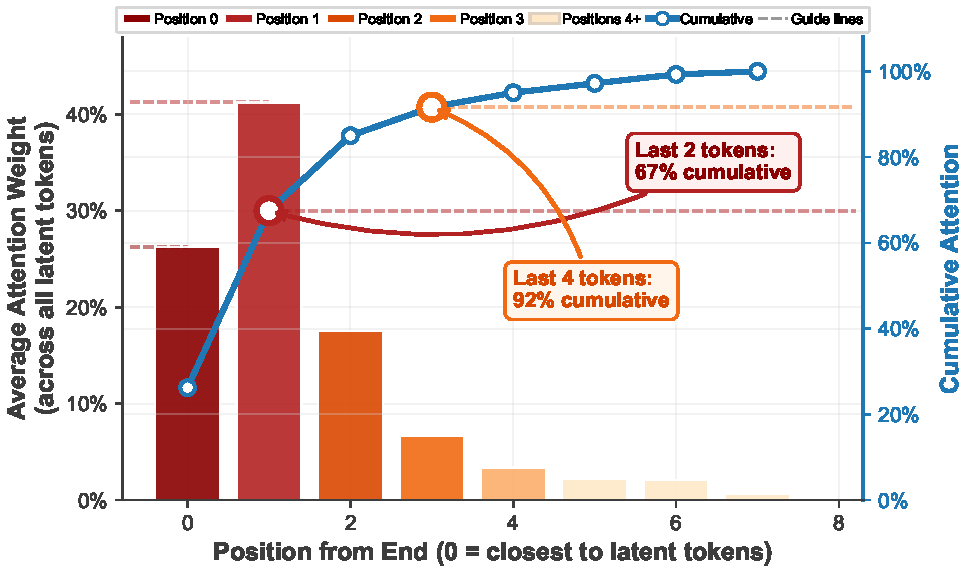
\includegraphics[width=\linewidth]{imgs/cross_attention_bias.pdf}
    \caption{\textbf{Cross-attention weight distribution across different number of context tokens.}
    Position 0 denotes the \textbf{last} token before latent synthesis, position 1 the \textbf{second-to-last}, and so on.
    The model concentrates attention on the most recent 1--2 positions regardless of available context.}
    \label{fig:attention_heatmap}
    \vspace{-5mm}
\end{figure}


A key design choice in PaCT is the number of context tokens used as keys and values for cross-attention
during latent synthesis. Table~\ref{tab:gpt2_gsm8k_context} shows that expanding this context beyond a
small window does not improve performance and can even degrade it. Figure~\ref{fig:attention_heatmap}
explains this behavior: regardless of available context length, cross-attention concentrates on the most
recent hidden states.

This aligns with prior observations that Transformer attention exhibits a strong inductive bias toward
recency~\citep{press2021train}. In PaCT, this bias is amplified because latent synthesis attends not only
to text tokens but also to latent states from previous stages, which already summarize the cumulative
context. As a result, attending to recent latents provides access to relevant historical information
without requiring long text-level context.

Together, these results justify a restricted context window for latent synthesis, which aligns with the
model’s learned attention bias while improving computational efficiency.


\subsection{Perturbing PaCT's latent states}
\label{sec:perturbation_analysis}

Having established that each reasoning stage contributes to PaCT's final prediction
(Sec.~\ref{sec:stage_ablation}) and that latent trajectories carry a meaningful confidence signal
(Sec.~\ref{sec:latent_decoding}), we now probe what the latent reasoning states actually encode by
intervening on them directly at inference time. The guiding hypothesis is simple: if the latents
carry task-relevant reasoning information, destructive perturbations that erase or replace them
should reduce accuracy substantially, whereas structure-preserving noise should be largely absorbed.

\paragraph{Probes.}
We apply five inference-time interventions to a trained PaCT model on GSM8k, without any additional
training: (i) \emph{zeroing}, where every latent state is replaced with the zero vector;
(ii) \emph{random-norm replacement}, where each latent is replaced with a Gaussian random vector
rescaled to match the empirical latent norm; (iii) \emph{cross-example swap}, where latents
synthesized for a randomly paired, unrelated example are substituted for the current ones;
(iv) \emph{no-prompt decode}, where answer tokens are prevented from attending back to the question
prefix during decoding so that the answer must be reconstructed from the latent states alone; and
(v) \emph{additive Gaussian noise} $\varepsilon \sim \mathcal{N}(0, \sigma^2 I)$ added to every
latent, swept over $\sigma \in \{0.01, 0.05, 0.1, 1.0\}$.

\begin{table}[t]
\centering
\small
\caption{\textbf{Perturbing PaCT's latent reasoning states on GSM8k.}
Destructive interventions (zeroing, random-norm replacement, cross-example swap) collapse accuracy,
while structure-preserving Gaussian noise is largely absorbed. Restricting answer decoding to attend
only to latent states (no-prompt decode) also collapses accuracy, indicating that the latents encode
information not redundantly present in the prompt.}
\label{tab:latent_perturbation}
\begin{tabular}{@{}lc@{}}
\toprule
Condition & Accuracy (\%) \\
\midrule
PaCT (clean)                                        & 34.40 \\
\midrule
Zero all latents                                    & 7.80  \\
Random vectors, matched norm                        & 8.77  \\
Swap latents across examples                        & 4.27  \\
No-prompt decode (answer attends only to latents)   & 7.40  \\
\midrule
Gaussian noise, $\sigma{=}0.01$                     & 33.62 \\
Gaussian noise, $\sigma{=}0.05$                     & 33.62 \\
Gaussian noise, $\sigma{=}0.10$                     & 33.78 \\
Gaussian noise, $\sigma{=}1.00$                     & 31.77 \\
\bottomrule
\end{tabular}
\end{table}

Table~\ref{tab:latent_perturbation} summarizes the results. Three observations follow.
\emph{First, destructive perturbations collapse performance.} Zeroing ($7.80\%$), random-norm
replacement ($8.77\%$), and cross-example swap ($4.27\%$) each reduce accuracy by more than $25$
absolute points from the $34.40\%$ clean baseline, so the latent states are load-bearing for PaCT's
predictions rather than acting as passive padding.
\emph{Second, the latent pathway carries non-redundant information.} When answer decoding is
restricted to attend only to the latent states, accuracy falls to $7.40\%$, showing that the latents
encode signal that the prompt path alone cannot reconstruct.
\emph{Third, latents occupy a structured submanifold.} Gaussian perturbations stay close to the
clean baseline across the entire sweep ($33.62\%$ at $\sigma{=}0.01$, $33.62\%$ at $\sigma{=}0.05$,
$33.78\%$ at $\sigma{=}0.1$, and $31.77\%$ even at $\sigma{=}1.0$), whereas random unit-norm
replacements — which share the noise's isotropy but destroy the learned directions — collapse it
($8.77\%$). The latents therefore live on a learned submanifold along which small,
structure-preserving perturbations are absorbed, while arbitrary high-magnitude directions are not.
These probes are run at the GPT-2 scale on GSM8k.

\subsection{Out-of-distribution generalization}
\label{sec:ood_transfer}

To assess whether PaCT's improvements on GSM8k reflect genuine arithmetic reasoning rather than
GSM8k-specific regularities, we evaluate GSM8k-trained checkpoints zero-shot on three held-out math
benchmarks: GSM-HARD, MultiArith, and SVAMP. Coconut results are obtained by rerunning the released
Coconut~\cite{hao2024training} implementation under its best reported configuration for this
setting, and for MultiArith we use the same evaluation subset adopted in prior continuous latent
reasoning work, ensuring an apples-to-apples comparison.

\begin{table}[t]
\centering
\small
\caption{\textbf{Out-of-distribution generalization.}
All models are trained on GSM8k and evaluated zero-shot on three held-out math benchmarks. PaCT
matches or exceeds Coconut on every split.}
\label{tab:ood_transfer}
\begin{tabular}{lcc}
\toprule
Dataset & PaCT (\%) & Coconut (\%) \\
\midrule
GSM-HARD                  & \textbf{7.88}  & 7.90  \\
MultiArith                & \textbf{82.34} & 82.00 \\
SVAMP                     & \textbf{37.67} & 36.40 \\
\bottomrule
\end{tabular}
\end{table}

As shown in Table~\ref{tab:ood_transfer}, PaCT matches or exceeds Coconut across all three OOD
benchmarks. This suggests that the improvements observed on GSM8k translate to related but held-out
distributions rather than being tied to GSM8k-specific artifacts.


% ###################################################################
% ###################################################################
% ###################################################################




\section{Limitations and Future Scope}

While PaCT substantially improves the efficiency and scalability of continuous latent reasoning, it does not yet surpass language-based chain-of-thought reasoning in absolute accuracy on all tasks. Our study focuses on supervised, text-only reasoning, and extending PaCT to multimodal settings is an important direction for future work. Integrating PaCT-style latent reasoning into reinforcement learning and policy optimization frameworks such as GRPO, as well as understanding its interaction with pretraining objectives and long-horizon decision-making, may further improve the generality and robustness of latent reasoning systems also aiding in surpassing the COT upper limit otherwise more naturally present with SFT-based methods.

\paragraph{Exploiting the latent submanifold.}
Our perturbation analysis in Section~\ref{sec:perturbation_analysis} shows that PaCT's latent states are tightly concentrated on a low-dimensional, structure-preserving submanifold: additive Gaussian noise is absorbed across two orders of magnitude of $\sigma$, while norm-matched random replacements — which leave the manifold — collapse accuracy. This is a finding our perturbation experiments made visible, and it suggests an explicit modeling direction. Future methods could parameterize latent synthesis to operate directly in the learned submanifold (for instance via a low-rank or VQ-style projection, or a normalizing-flow prior over latent directions), rather than allowing the full ambient dimensionality and relying on training dynamics to discover the submanifold implicitly. Such a parameterization could improve sample efficiency, reduce redundancy across within-stage latents, and provide a more controllable interface for interpretability and intervention. This is just one direction of thought and the findings can be interpreted in multiple other ways.

\paragraph{From curriculum-based training to learned latent objectives at scale.}
The same perturbation analysis suggests a natural caveat about scaling. At the GPT-2 scale we study here, a curriculum that progressively replaces textual CoT tokens with latent reasoning stages is effective at inducing a structured latent submanifold. Prior work that has evaluated faithfulness of Coconut-style latents at much larger scales, however, has reported weaker latent-intervention effects — a pattern that we interpret not as evidence against latent reasoning per se, but as a signal that curriculum-based supervision, which effectively commits each latent to a fixed role early in training, may not be the right inductive lever for larger models with substantially more expressive latent spaces. A promising future direction is to replace the token-replacement curriculum with an explicit latent-space learning objective that (i) does not pin each latent to a single canonical role, (ii) shapes the latent submanifold directly through geometric or information-theoretic regularizers, and (iii) can be combined with the parallel stage-wise synthesis introduced in this paper. We see the submanifold structure documented here as the first concrete handle for designing such a training objective.


\section{Conclusion}
\label{sec:conclusion}

In this paper, we introduce Parallel Continuous Thought (PaCT), a new paradigm for continuous latent reasoning that removes the need for recurrent latent state propagation. PaCT constructs reasoning through stage-wise, parallel latent resynthesis, enabling efficient depth without incurring the serial bottlenecks of latent unrolling. Across a range of reasoning tasks and model scales, PaCT matches or improves the accuracy of prior continuous thought methods while achieving substantial gains in training and inference efficiency. Beyond performance, our analyses reveal that PaCT learns stage-specialized latent representations, exhibits more stable internal dynamics, and benefits systematically from increased reasoning depth. Together, these results challenge the assumption that effective latent reasoning must rely on propagating latent states across steps through recurrent unrolling, and suggest that repeated, context-grounded latent resynthesis offers a scalable alternative.  We hope this work motivates further exploration of non-recurrent latent reasoning architectures for building more efficient and robust reasoning systems.





% We introduced \emph{Parallel Continuous Thought} (PaCT), a reformulation of continuous latent reasoning that eliminates the recurrent latent-unrolling bottleneck present in Coconut-style training. PaCT organizes latent reasoning into stages and re-synthesizes a set of latent reasoning states in parallel at each stage from the current textual context, enabling efficient hardware parallelism while preserving standard causal decoding.

% Empirically, PaCT matches or exceeds Coconut across GSM8k, ProntoQA, and ProsQA while delivering substantial training-time reductions, and the same efficiency gains persist when scaling to larger base models. We further showed that PaCT’s gains are not merely computational: stage ablations reveal that each stage contributes meaningful signal to the final prediction; latent similarity diagnostics indicate that PaCT’s stages encode more distinct information than recurrent unrolling; vocabulary-space probes expose coherent intermediate-to-final progressions in correct predictions; and ICR analyses suggest that PaCT stabilizes internal dynamics earlier than Coconut. Finally, a context-length ablation supports the design choice that latent synthesis primarily benefits from the most recent hidden states.

% Overall, PaCT demonstrates that continuous latent reasoning can be made substantially more scalable by removing recurrent latent dependencies, while simultaneously promoting stage-wise structure in the latent computation. This positions PaCT as a practical and extensible foundation for training-efficient latent reasoning in larger models and more complex settings.


% In the unusual situation where you want a paper to appear in the
% references without citing it in the main text, use \nocite
% \nocite{langley00}

\bibliography{example_paper}
\bibliographystyle{icml2026}

% \newpage
% \appendix
% \onecolumn
% \section{You \emph{can} have an appendix here.}

% Supplimentary section

% \subsection{Extended Latent Decoding Examples}
% \label{sec:supp_latent_decode}

% We present additional examples of latent-to-token decoding to supplement the analysis in Section~\ref{sec:latent_decoding}.

% \vspace{1em}
% \noindent\fbox{\parbox{0.97\textwidth}{
% \textbf{Example S1} \hfill \textcolor{green!60!black}{\textbf{Correct}} \\[0.5em]
% \textbf{Question:} Maggie went to Lou's aquarium and saw 100 goldfish in the aquarium. She asked if she could take some home to care for, and she was allowed to catch half of them. While using a catching net, she caught 3/5 of the total number of goldfish she was allowed to take home. How many goldfish does Maggie remain with to catch to get the total number she was allowed to take home? \\[0.3em]
% \textbf{Ground Truth CoT:} $100 \times \frac{1}{2} = 50$ \quad$\rightarrow$\quad $50 \times \frac{3}{5} = 30$ \quad$\rightarrow$\quad $50 - 30 = 20$ \\[0.3em]
% \textbf{Predicted:} 20 \quad \textbf{GT:} 20 \\[0.5em]
% \begin{tabular}{c|cccccc}
% & L0 & L1 & L2 & L3 & L4 & L5 \\
% \hline
% Token & \textbf{50} & \textbf{50} & \textbf{30} & \textbf{30} & \textbf{20} & \textbf{20} \\
% Prob & 13\% & 14\% & 13\% & 20\% & 55\% & 56\% \\
% \end{tabular} \\[0.3em]
% \textit{Interpretation:} Perfect alignment with CoT---L0--L1 encode allowed amount (50), L2--L3 encode caught amount (30), L4--L5 compute remainder (20).
% }}

% \vspace{1em}
% \noindent\fbox{\parbox{0.97\textwidth}{
% \textbf{Example S2} \hfill \textcolor{green!60!black}{\textbf{Correct}} \\[0.5em]
% \textbf{Question:} Mitchell is trying to chew as many pieces of gum at once as he can. He has 8 packets of gum. There are 7 pieces in each. If he chews all the gum except for 2 pieces, how many pieces does he chew at once? \\[0.3em]
% \textbf{Ground Truth CoT:} $8 \times 7 = 56$ \quad$\rightarrow$\quad $56 - 2 = 54$ \\[0.3em]
% \textbf{Predicted:} 54 \quad \textbf{GT:} 54 \\[0.5em]
% \begin{tabular}{c|cccccc}
% & L0 & L1 & L2 & L3 & L4 & L5 \\
% \hline
% Token & \textbf{56} & \textbf{56} & \textbf{54} & \textbf{54} & \textbf{54} & \textbf{54} \\
% Prob & 5.2\% & 6.5\% & 25\% & 50\% & 87\% & 83\% \\
% \end{tabular} \\[0.3em]
% \textit{Interpretation:} L0--L1 compute total pieces (56), L2--L5 subtract and converge to final answer (54) with high confidence.
% }}

% \vspace{1em}
% \noindent\fbox{\parbox{0.97\textwidth}{
% \textbf{Example S3} \hfill \textcolor{red}{\textbf{Incorrect}} \\[0.5em]
% \textbf{Question:} Roman and Remy took separate showers. Remy used 1 more gallon than 3 times the number of gallons that Roman used for his shower. Together the boys used 33 gallons of water. How many gallons did Remy use? \\[0.3em]
% \textbf{Ground Truth CoT:} Let Roman $= x$, Remy $= 3x + 1$. \quad $x + 3x + 1 = 33$ \quad$\rightarrow$\quad $x = 8$ \quad$\rightarrow$\quad Remy $= 25$ \\[0.3em]
% \textbf{Predicted:} 26.25 \quad \textbf{GT:} 25 \\[0.5em]
% \begin{tabular}{c|cccccc}
% & L0 & L1 & L2 & L3 & L4 & L5 \\
% \hline
% Token & 34 & 34 & 9 & 9 & \textbf{25} & \textbf{25} \\
% Prob & 11\% & 12\% & 7.5\% & 8.6\% & 22\% & 26\% \\
% \end{tabular} \\[0.3em]
% \textit{Interpretation:} Latents arrive at the correct answer (25) by L4--L5, but the final decoding produces 26.25---a mismatch between latent representation and output generation.
% }}

% \vspace{1em}
% \noindent\fbox{\parbox{0.97\textwidth}{
% \textbf{Example S4} \hfill \textcolor{red}{\textbf{Incorrect}} \\[0.5em]
% \textbf{Question:} When Suzy the librarian sat at her desk on Wednesday morning, she had 98 books ready for checkout. The same day, 43 books were checked out. The following day, 23 books were returned, but 5 books were checked out. On Friday, 7 books were returned. How many books did Suzy have? \\[0.3em]
% \textbf{Ground Truth CoT:} $98 - 43 = 55$ \quad$\rightarrow$\quad $55 + 23 = 78$ \quad$\rightarrow$\quad $78 - 5 = 73$ \quad$\rightarrow$\quad $73 + 7 = 80$ \\[0.3em]
% \textbf{Predicted:} 119 \quad \textbf{GT:} 80 \\[0.5em]
% \begin{tabular}{c|cccccc}
% & L0 & L1 & L2 & L3 & L4 & L5 \\
% \hline
% Token & 69 & 69 & 76 & 72 & 70 & 70 \\
% Prob & 3.6\% & 3.4\% & 0.9\% & 1.6\% & 11\% & 9.3\% \\
% \end{tabular} \\[0.3em]
% \textit{Interpretation:} Multi-step tracking fails---model approximates values near the answer (70) but never reaches 80. Consistently low probabilities indicate uncertainty throughout.
% }}

% \vspace{1em}
% \noindent\fbox{\parbox{0.97\textwidth}{
% \textbf{Example S5} \hfill \textcolor{red}{\textbf{Incorrect}} \\[0.5em]
% \textbf{Question:} Elsa and her sister watch an opera show every year at Central City Opera. Last year, opera seating cost \$85 per ticket. This year, it costs \$102. What is the percent increase in the cost of each ticket? \\[0.3em]
% \textbf{Ground Truth CoT:} $102 - 85 = 17$ \quad$\rightarrow$\quad $\frac{17}{85} \times 100 = 20\%$ \\[0.3em]
% \textbf{Predicted:} 12 \quad \textbf{GT:} 20 \\[0.5em]
% \begin{tabular}{c|cccccc}
% & L0 & L1 & L2 & L3 & L4 & L5 \\
% \hline
% Token & 73 & 73 & . & . & 12 & 12 \\
% Prob & 3.5\% & 3.1\% & 12\% & 18\% & 25\% & 24\% \\
% \end{tabular} \\[0.3em]
% \textit{Interpretation:} L0--L1 encode an unexplained value (73). L2--L3 produce non-numeric tokens (``.''), indicating reasoning breakdown. The model commits to wrong answer (12) without computing the correct percentage.
% }}

% \begin{figure}[H]
% \centering
% \fbox{%
% \parbox{0.97\columnwidth}{
% \textbf{Example 1} \hfill \textcolor{green!60!black}{\textbf{Correct}} \\[0.5em]
% \textbf{Question:} A set of 7 spoons costs \$21. If each spoon would be sold separately, how much would 5 spoons cost? \\[0.3em]
% \textbf{Ground Truth CoT:} $21 \div 7 = 3$ \quad$\rightarrow$\quad $5 \times 3 = 15$ \\[0.3em]
% \textbf{Predicted:} 15 \quad \textbf{GT:} 15 \\[0.5em]
% \begin{tabular}{c|cccccc}
% & L0 & L1 & L2 & L3 & L4 & L5 \\
% \hline
% Token & \textbf{3} & \textbf{3} & \textbf{15} & \textbf{15} & \textbf{15} & \textbf{15} \\
% Prob & 62\% & 66\% & 37\% & 60\% & 84\% & 92\% \\
% \end{tabular} \\[0.3em]
% \textit{Interpretation:} L0--L1 encode the intermediate unit price (3), then L2--L5 converge to the final answer (15).
% }}
% \end{figure}

% \begin{figure}[H]
% \centering
% \fbox{%
% \parbox{0.97\columnwidth}{
% \textbf{Example 2} \hfill \textcolor{green!60!black}{\textbf{Correct}} \\[0.5em]
% \textbf{Question:} Travis wants to fly to Australia. The regular tickets cost about \$2000. As Travis is a student, he will get a 30\% discount on this price. How much does he need to pay for his ticket? \\[0.3em]
% \textbf{Ground Truth CoT:} $2000 \times 0.30 = 600$ \quad$\rightarrow$\quad $2000 - 600 = 1400$ \\[0.3em]
% \textbf{Predicted:} 1400 \quad \textbf{GT:} 1400 \\[0.5em]
% \begin{tabular}{c|cccccc}
% & L0 & L1 & L2 & L3 & L4 & L5 \\
% \hline
% Token & 1400 & 1400 & 1400 & 1400 & 1400 & 1400 \\
% Prob & 2.4\% & 5.3\% & 28\% & 41\% & 89\% & 92\% \\
% \end{tabular} \\[0.3em]
% \textit{Interpretation:} The answer emerges early but with low confidence; probability sharpens dramatically from 2\% to 92\% across stages.
% }}
% \end{figure}

% \begin{figure}[H]
% \centering
% \fbox{%
% \parbox{0.97\columnwidth}{
% \textbf{Example 4} \hfill \textcolor{red}{\textbf{Incorrect}} \\[0.5em]
% \textbf{Question:} John cuts his grass to 2 inches. It grows 0.5 inches per month. When it gets to 4 inches he cuts it back down to 2 inches. It costs \$100 to get his grass cut. How much does he pay per year? \\[0.3em]
% \textbf{Ground Truth CoT:} $4-2=2$ \quad$\rightarrow$\quad $2 \div 0.5 = 4$ months \quad$\rightarrow$\quad $12 \div 4 = 3$ cuts \quad$\rightarrow$\quad $100 \times 3 = 300$ \\[0.3em]
% \textbf{Predicted:} 200 \quad \textbf{GT:} 300 \\[0.5em]
% \begin{tabular}{c|cccccc}
% & L0 & L1 & L2 & L3 & L4 & L5 \\
% \hline
% Token & / & / & 200 & 200 & 200 & 5000 \\
% Prob & 0.5\% & 0.4\% & 6.2\% & 11\% & 5.9\% & 8.5\% \\
% \end{tabular} \\[0.3em]
% \textit{Interpretation:} Model fails to compute cutting frequency. Low, unstable probabilities throughout indicate uncertain reasoning. Final latent diverges entirely.
% }}
% \end{figure}

% \vspace{1em}
% These supplementary examples reinforce the main findings: correct predictions exhibit clear intermediate-to-final progressions with sharpening confidence, while incorrect predictions show fragmented reasoning, wrong intermediates, or latent-output mismatches.

% %\colorbox{red}{BELOW Inference Time Plot. @Prakash bhaiya pls paste it to appropriate location}
% % \begin{figure}[h!]
% %   \centering
% %   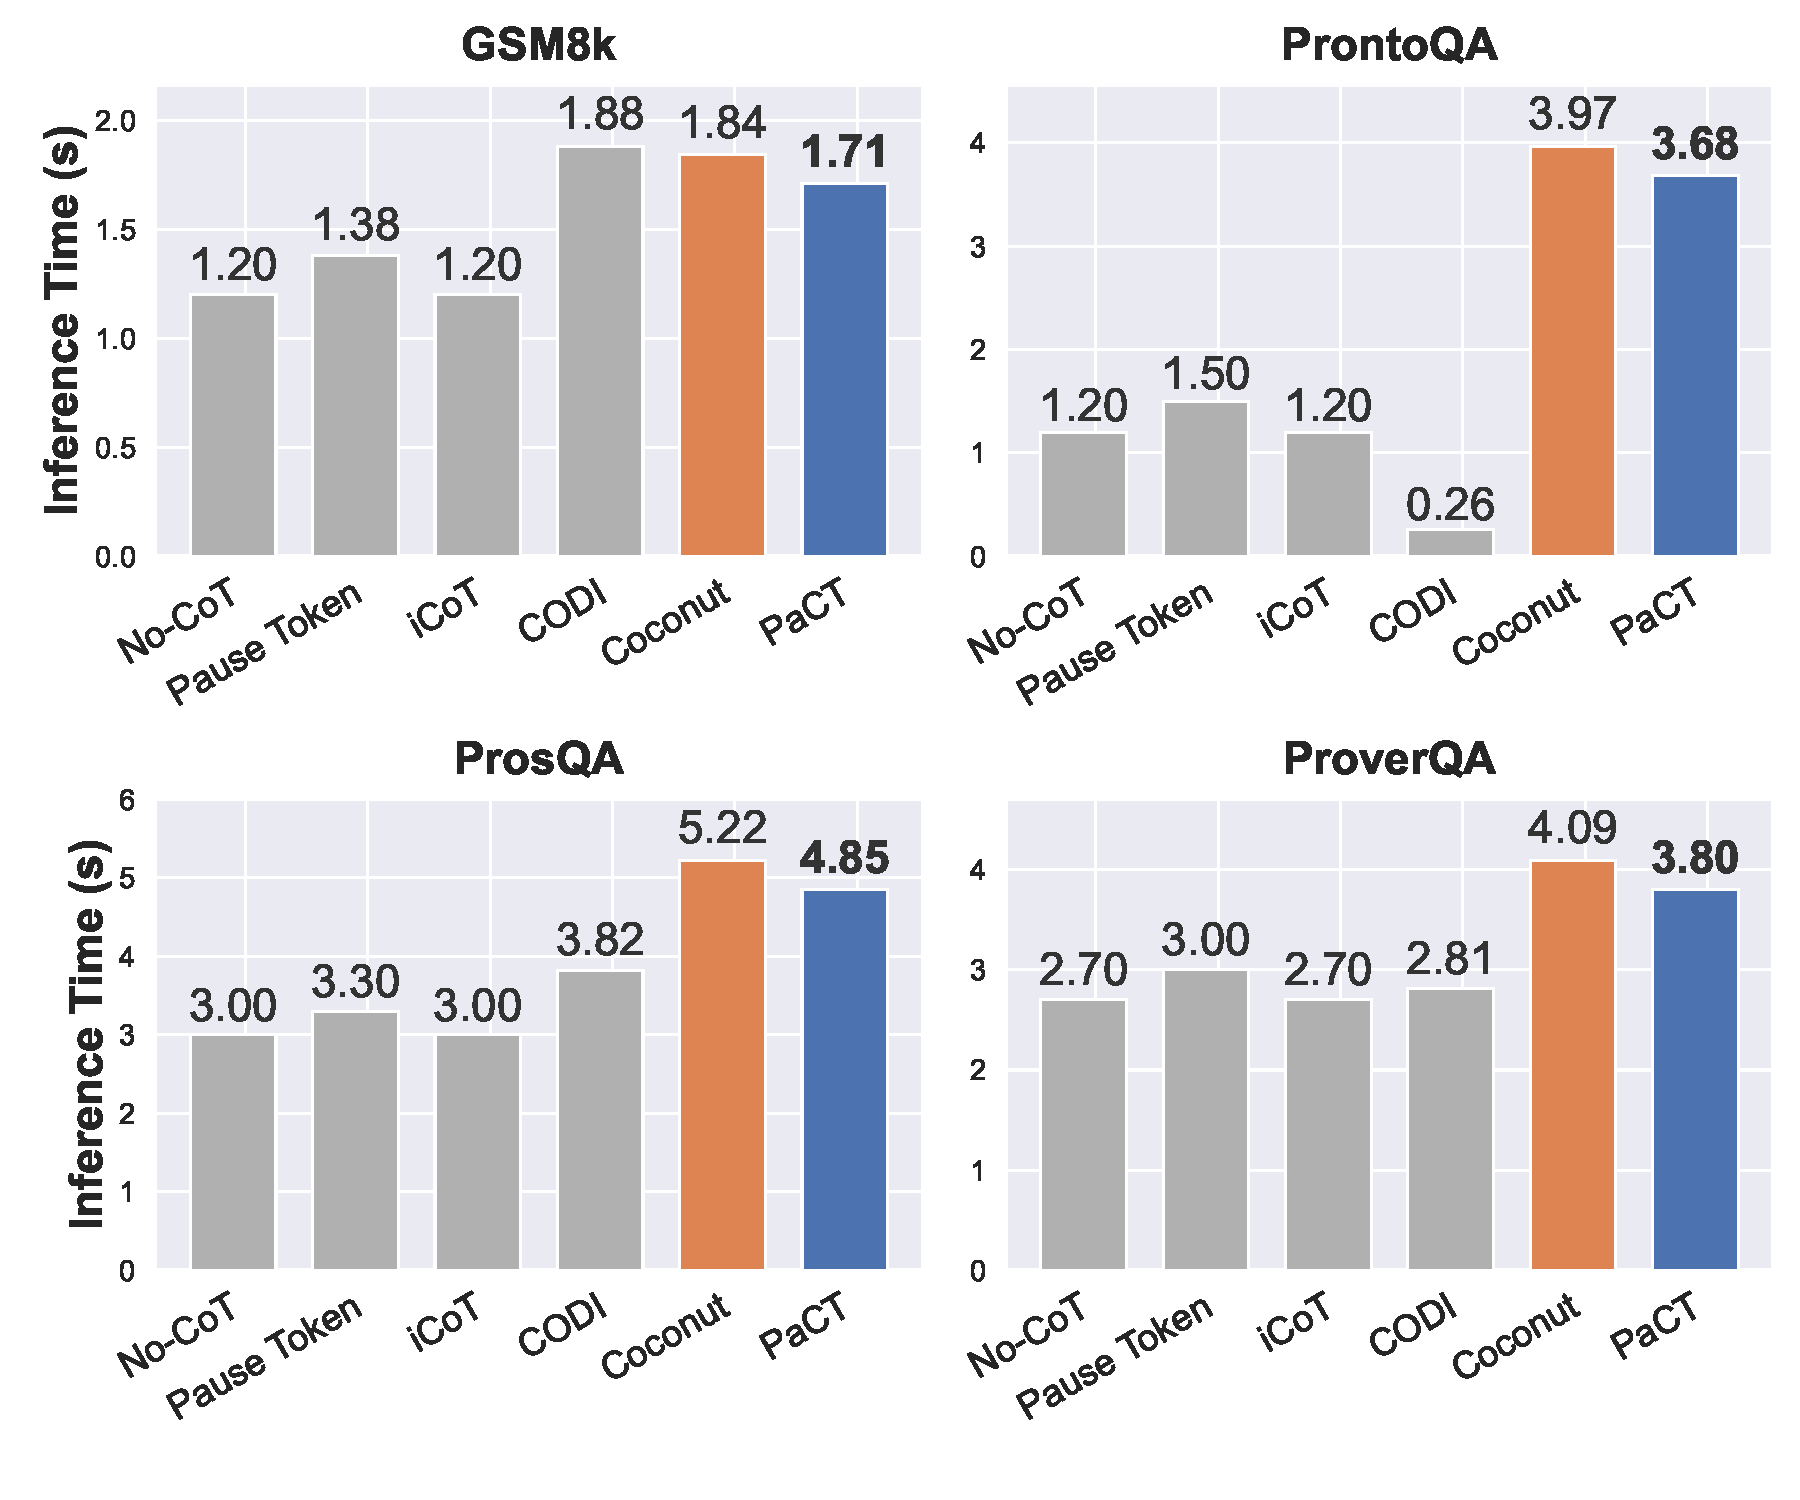
\includegraphics[width=\linewidth]{imgs/inference_times.pdf}
% %       \caption{Inference time (in seconds) for different reasoning methods across four benchmarks. PaCT demonstrates consistently lower latency compared to Coconut while maintaining competitive performance over baseline approaches.}
% %   \label{fig:inference_time}
% % \end{figure}
% %%%%%%%%%%%%%%%%%%%%%%%%%%%%%%%%%%%%%%%%%%%%%%%%%%%%%%%%%%%%%%%%%%%%%%%%%%%%%%%


% \section{Stability and initialization details}
% \label{app:stability}

% To stabilize optimization, we ground latent reasoning states in the task specification. Let $h_q$
% denote the hidden state of the final question token. We initialize the output projection of the latent
% synthesis cross-attention to zero and add $h_q$ as a residual to each latent state after synthesis.
% This ensures that, at initialization, all latent states correspond to grounded copies of the question
% representation and only deviate when learning discovers useful refinements.

% This grounding serves two purposes: (i) it anchors latent reasoning to the task context throughout
% training, and (ii) it prevents unstructured accumulation of latent history by ensuring that each
% stage depends only on the current textual context and a fixed task representation.

% \section{Attention masking and causal structure}
% \label{app:masking}

% We enforce the following attention constraints:
% \begin{enumerate}
%   \item Text tokens attend causally to earlier text tokens.
%   \item Text tokens do not attend to future latent states.
%   \item Latent states attend to all previous text tokens and to other latent states within the same
%   stage bidirectionally.
%   \item Answer tokens attend to all prior text tokens and all latent states from previous stages.
% \end{enumerate}
% This realizes a \emph{Text $\rightarrow$ Latents $\rightarrow$ Text} pattern while preserving
% autoregressive decoding and preventing label leakage.

% \section{Training algorithm}
% \label{app:algorithm}

% Algorithm~\ref{alg:pact_training} provides the full curriculum training procedure for PaCT.

% \begin{algorithm}[h]
% \caption{Curriculum training for PaCT}
% \label{alg:pact_training}
% \begin{algorithmic}[1]
% \Require Dataset $\mathcal{D}$, curriculum schedule $\{m_s,S_s\}$, slots $L$, parameters $\theta$, stepsize $\eta$
% \For{$s=0,\dots,S_{\max}$}
%   \For{$(q,r,a)\sim \mathcal{D}$}
%     \State Replace first $m_s$ rationale tokens in $r$ with $S_s$ latent stages
%     \State $x \leftarrow [\,q;\ \tilde{r}_s;\ a\,]$
%     \State Compute $p_\theta(\cdot\mid x)$ and latent states $Z'^{(1:S_s)}$
%     \State Update $\theta \leftarrow \theta - \eta \nabla_\theta \mathcal{L}(\theta)$
%   \EndFor
% \EndFor
% \end{algorithmic}
% \end{algorithm}


% \begin{figure}[h!]
%   \centering
%   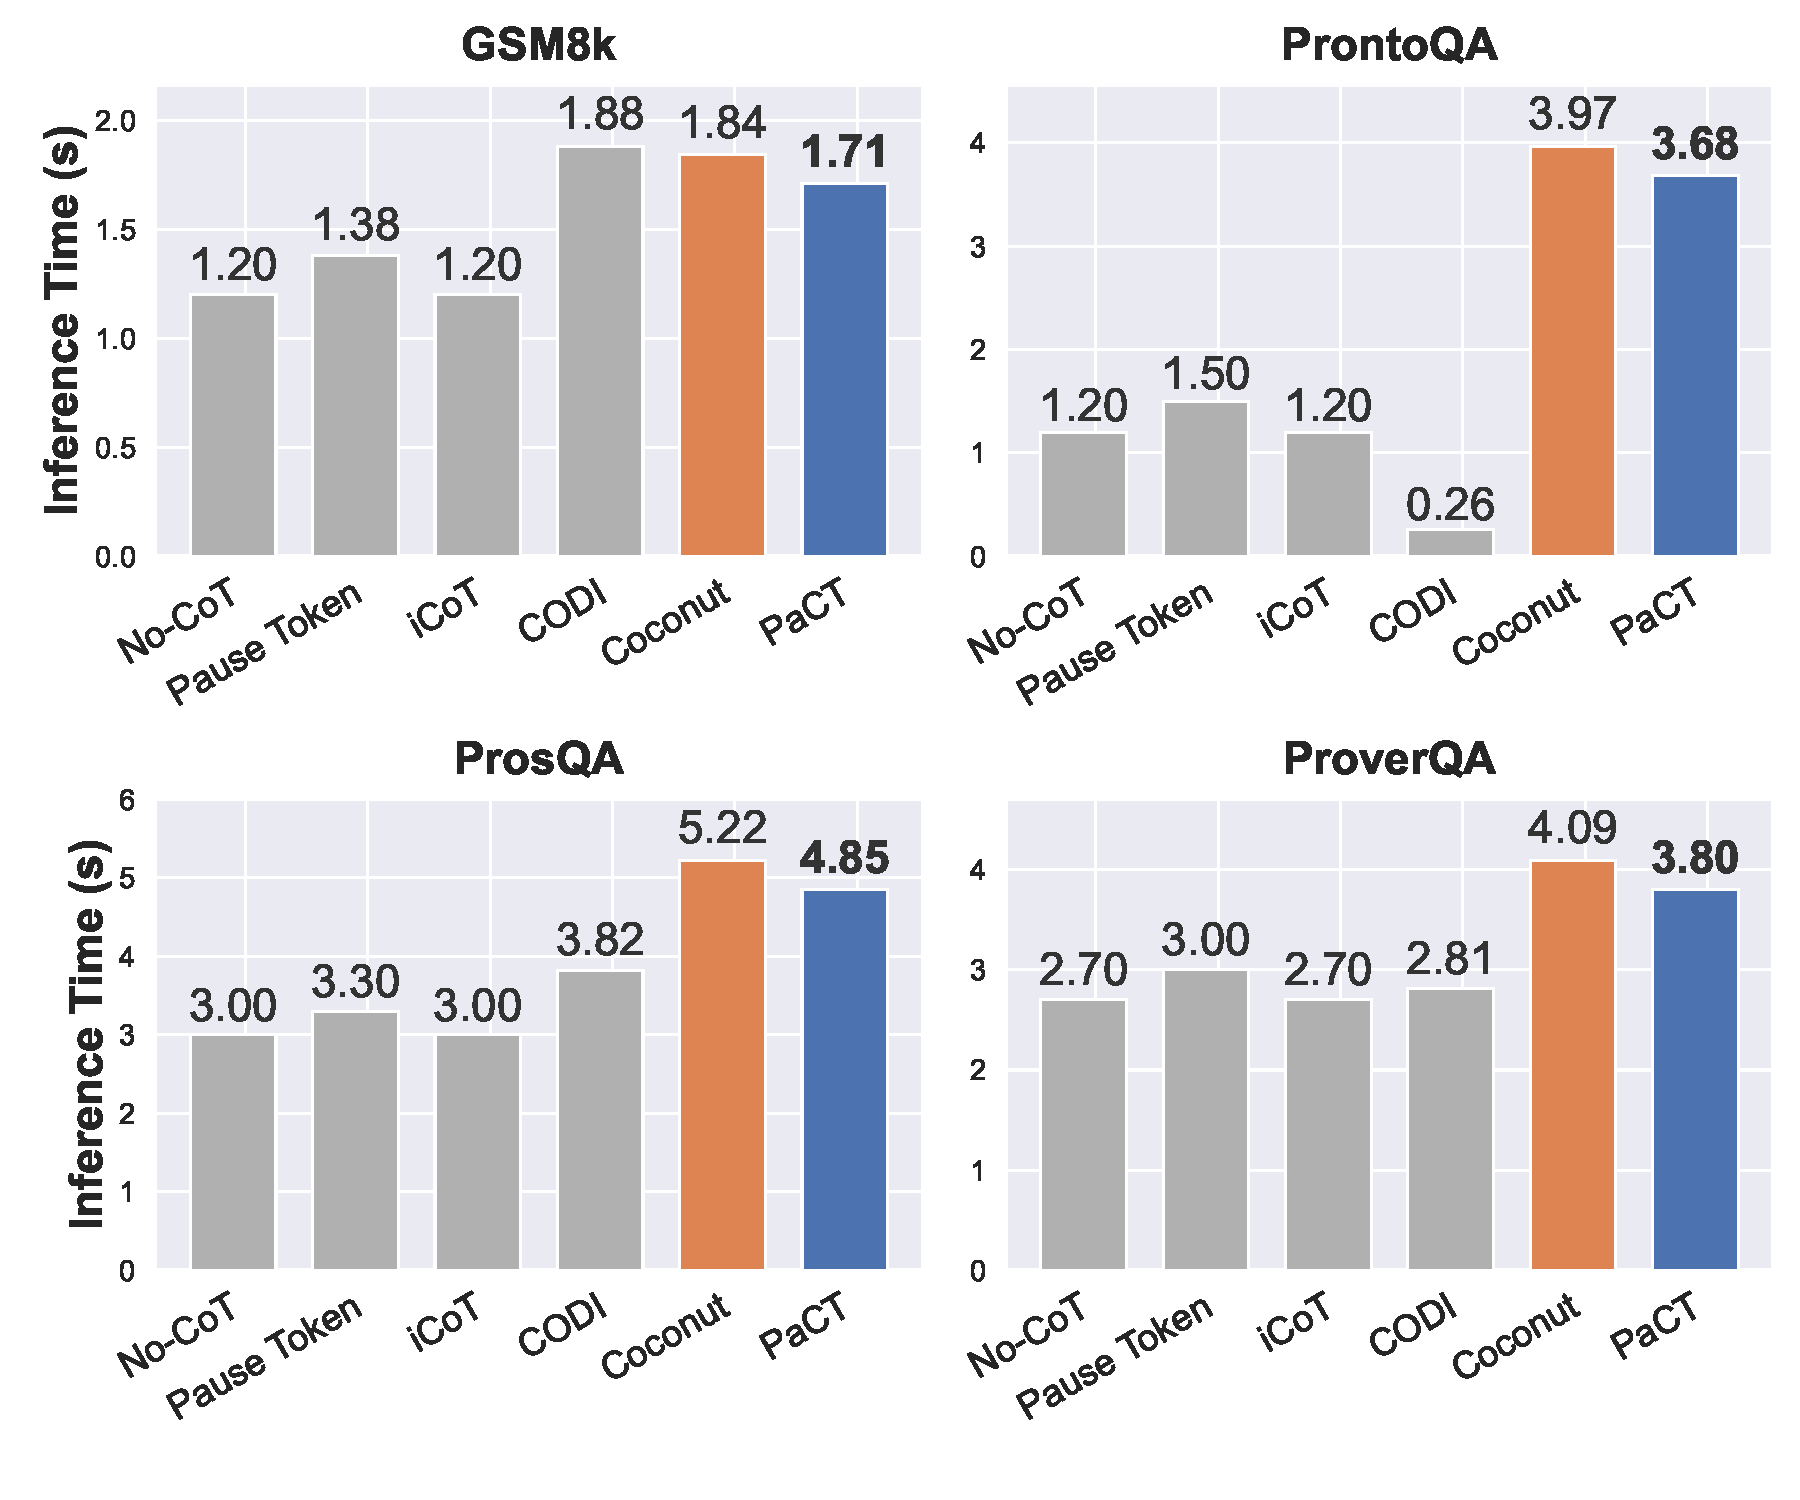
\includegraphics[width=\linewidth]{imgs/inference_times.pdf}
%       \caption{Inference time (in seconds) for different reasoning methods across four benchmarks. PaCT demonstrates consistently lower latency compared to Coconut while maintaining competitive performance over baseline approaches.}
%   \label{fig:inference_time}
% \end{figure}


% \begin{subfigure}[b]{0.48\textwidth}
%         \centering
%         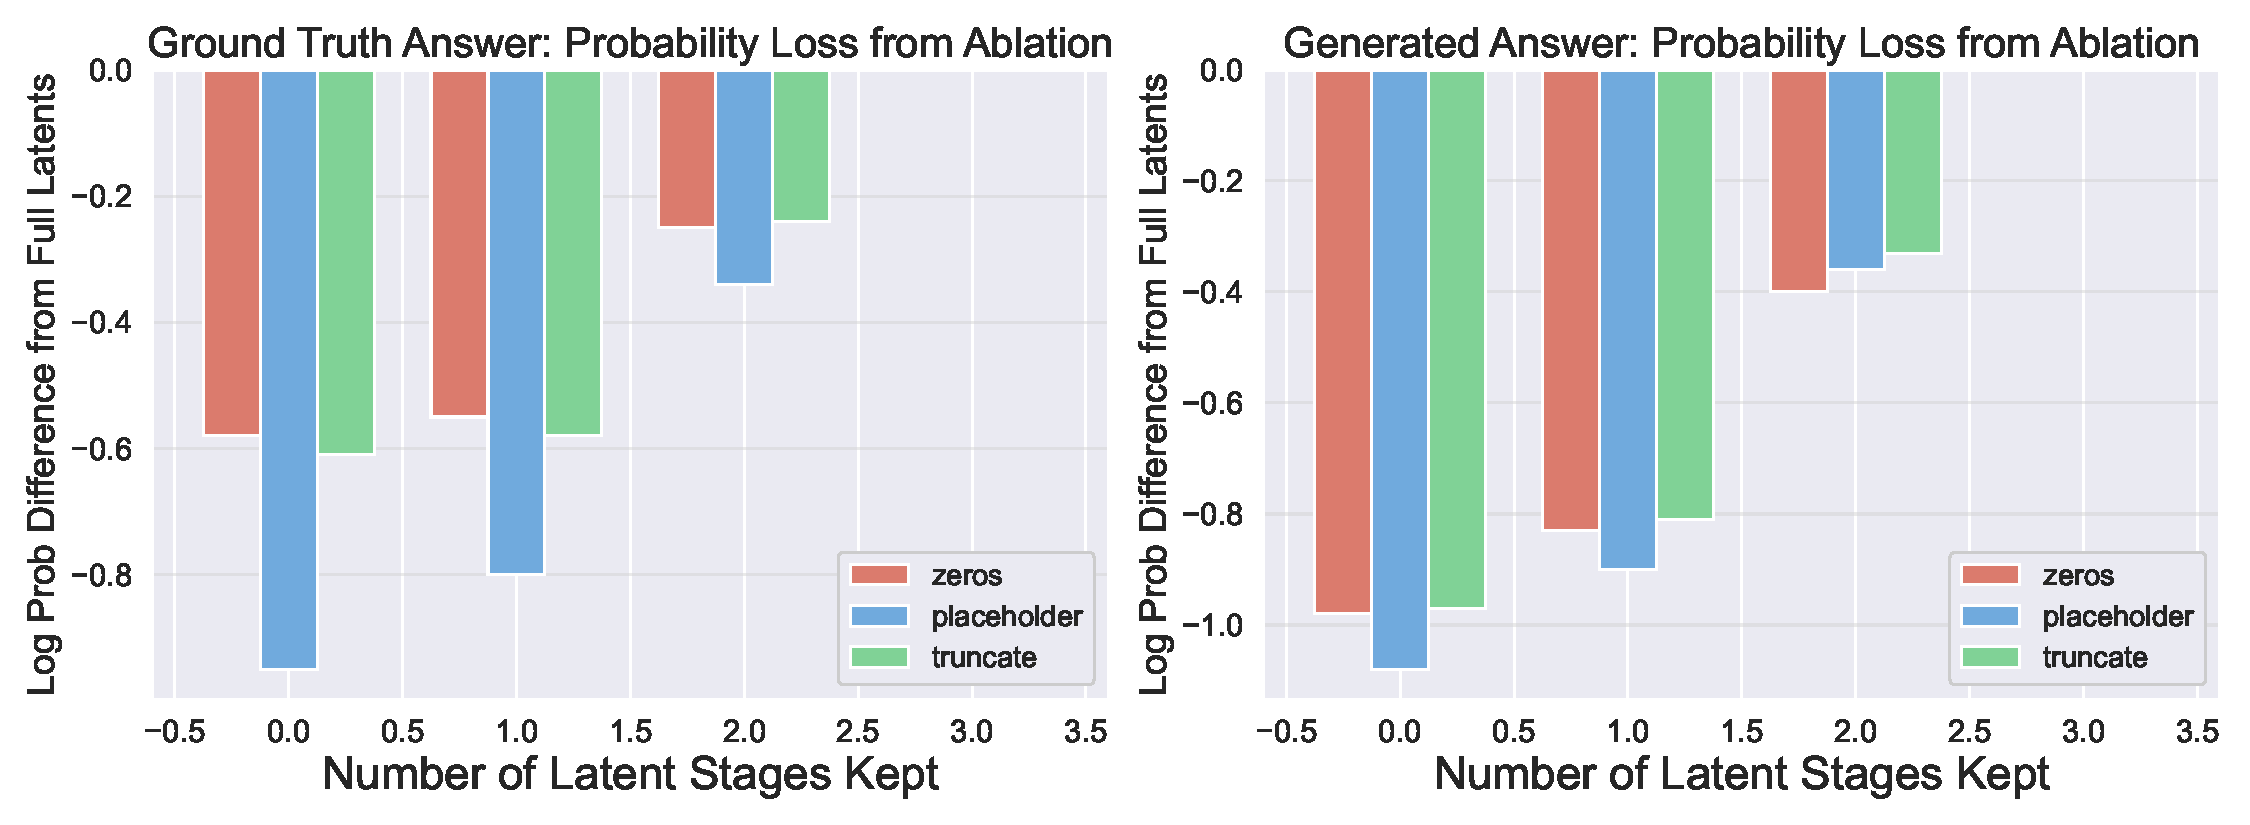
\includegraphics[width=\textwidth]{imgs/difference_from_baseline.pdf}
%         \caption{Difference from baseline}
%         \label{fig:ablation_diff}
%     \end{subfigure}


% \section{Additional Results and Ablations}
% \label{app:additional_results}

% \subsection{Log-probability drop relative to the full-latent baseline}
% \label{app:ablation_delta}

% \begin{figure}[t]
%   \centering
%   \includegraphics[width=\linewidth]{imgs/ablation_log_probs_delta.pdf}
%   \caption{\textbf{Stage ablation (relative view).} Log-probability drop relative to the full-latent baseline as a function of the number of stages retained. This view complements Fig.~\ref{fig:ablation_abs} by emphasizing the marginal value of additional stages. \textbf{[TODO: ensure the figure file name/path matches your repo; in the current PDF this plot appears as an additional figure-style panel.]}}
%   \label{fig:ablation_delta}
% \end{figure}

% \subsection{Depth sweep table for GSM8k}
% \label{app:depth_sweep_table}

% \begin{table}[t]
% \centering
% \small
% \caption{\textbf{Depth scaling on GSM8k (sweep).} Accuracy as a function of the number of stages on GSM8k with $c_{\text{thought}}=2$. \textbf{[TODO: clarify seeds/averaging for this sweep and reconcile the $S{=}3$ value with Table~\ref{tab:main_results} if they come from different runs.]}}
% \label{tab:stage_scaling}
% \begin{tabular}{l l c c}
% \toprule
% Method & Dataset & Accuracy (\%) & \# Stages \\
% \midrule
% Coconut & GSM8k & 34.2 & 3 \\
% PaCT    & GSM8k & 34.8 & 3 \\
% PaCT    & GSM8k & 36.6 & 6 \\
% PaCT    & GSM8k & 37.2 & 8 \\
% \bottomrule
% \end{tabular}
% \end{table}

% \subsection{Width and test-time truncation}
% \label{app:width_truncation}

% \begin{table}[t]
% \centering
% \small
% \caption{\textbf{Single-latent PaCT vs.\ dual-latent Coconut on GSM8k.} PaCT with $c_{\text{thought}}{=}1$ remains competitive with Coconut using $c_{\text{thought}}{=}2$, suggesting within-stage redundancy in PaCT.}
% \label{tab:1v2}
% \begin{tabular}{lcc}
% \toprule
% Model & $c_{\text{thought}}$ & Accuracy (\%) \\
% \midrule
% PaCT    & 1 & 33.20 \\
% Coconut & 2 & 32.00 \\
% \bottomrule
% \end{tabular}
% \end{table}

% \begin{table}[t]
% \centering
% \small
% \caption{\textbf{Test-time truncation of within-stage latents.} Accuracy when keeping only one of the two latent states per stage for a PaCT model trained with $c_{\text{thought}}=2$ and $S=3$ (GSM8k).}
% \label{tab:latent_redundancy}
% \begin{tabular}{lcc}
% \toprule
% Configuration & \# Latents & Accuracy (\%) \\
% \midrule
% Full model & 6 & 34.4 \\
% First of each stage (L0, L2, L4) & 3 & 31.6 \\
% Second of each stage (L1, L3, L5) & 3 & 31.6 \\
% \bottomrule
% \end{tabular}
% \end{table}

% \subsection{Effect of cross-attention context length}
% \label{app:context_length}

% \begin{table}[t]
%     \centering
%     \caption{\textbf{Effect of context length on GSM8k.} Accuracy for different numbers of context tokens (\texttt{num\_ctx}) used as keys/values in cross-attention.}
%     \label{tab:gpt2_gsm8k_context}
%     \begin{tabular}{lcc}
%         \toprule
%         Model & \texttt{num\_ctx} & Accuracy (\%) \\
%         \midrule
%         GPT-2 & 2   & 34.4 \\
%         GPT-2 & 4   & 33.0 \\
%         GPT-2 & 8   & 34.4 \\
%         GPT-2 & All & 30.6 \\
%         \bottomrule
%     \end{tabular}
% \end{table}

% \begin{figure}[t]
%   \centering
%   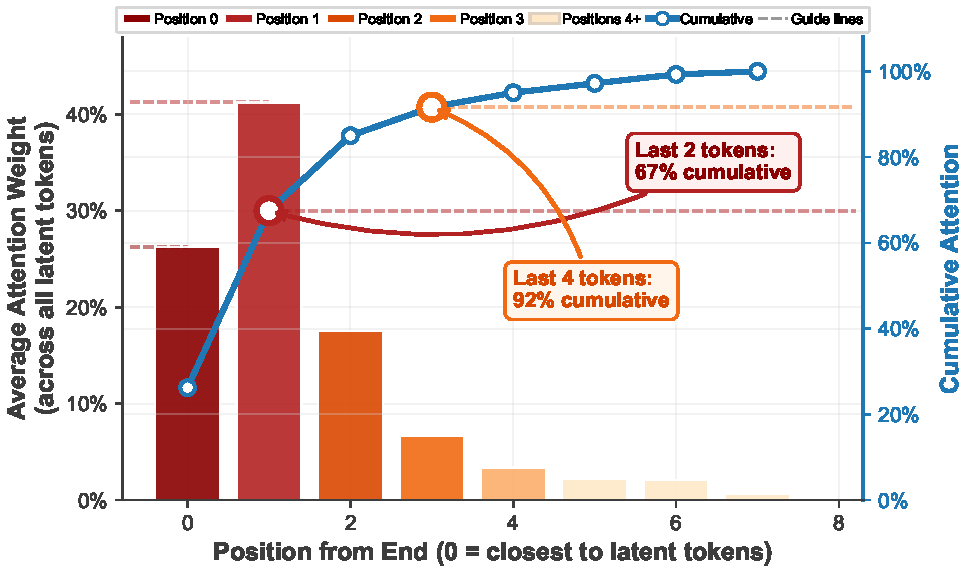
\includegraphics[width=\linewidth]{imgs/cross_attention_bias.pdf}
%   \caption{\textbf{Cross-attention concentrates on recent tokens.} Average attention weight as a function of position from the end of the prefix (0 = closest to the latent insertion point). Even with longer windows, attention mass concentrates on the last 1--2 hidden states, and cumulative attention saturates quickly.}
%   \label{fig:attention_heatmap}
% \end{figure}

% Table~\ref{tab:gpt2_gsm8k_context} shows that using the full prefix as cross-attention context degrades accuracy, while small windows remain strong. Figure~\ref{fig:attention_heatmap} explains this behavior: attention concentrates heavily on the most recent hidden states even when more context is available (e.g., $\sim$67\% mass on the last two tokens and $\sim$92\% on the last four). This supports the design choice of using a short window, which keeps latent synthesis lightweight without removing information the model actually uses.
% \textbf{[TODO: if you want a citation here, add one that supports ``recency dominance'' in autoregressive decoding; otherwise drop the sentence to avoid a weak citation.]}
% % =========================
% % Appendix: additional results
% % =========================

% \appendix

% \section{Additional Results and Ablations}
% \label{app:additional_results}

% \subsection{Log-probability drop relative to the full-latent baseline}
% \label{app:ablation_delta}

% \begin{figure}[t]
%   \centering
%   \includegraphics[width=\linewidth]{imgs/ablation_log_probs_delta.pdf}
%   \caption{\textbf{Stage ablation (relative view).} Log-probability drop relative to the full-latent baseline as a function of the number of stages retained. This view complements Fig.~\ref{fig:ablation_abs} by emphasizing the marginal value of additional stages. \textbf{[TODO: ensure the figure file name/path matches your repo; in the current PDF this plot appears as an additional figure-style panel.]}}
%   \label{fig:ablation_delta}
% \end{figure}

% \subsection{Depth sweep table for GSM8k}
% \label{app:depth_sweep_table}

% \begin{table}[t]
% \centering
% \small
% \caption{\textbf{Depth scaling on GSM8k (sweep).} Accuracy as a function of the number of stages on GSM8k with $c_{\text{thought}}=2$. \textbf{[TODO: clarify seeds/averaging for this sweep and reconcile the $S{=}3$ value with Table~\ref{tab:main_results} if they come from different runs.]}}
% \label{tab:stage_scaling}
% \begin{tabular}{l l c c}
% \toprule
% Method & Dataset & Accuracy (\%) & \# Stages \\
% \midrule
% Coconut & GSM8k & 34.2 & 3 \\
% PaCT    & GSM8k & 34.8 & 3 \\
% PaCT    & GSM8k & 36.6 & 6 \\
% PaCT    & GSM8k & 37.2 & 8 \\
% \bottomrule
% \end{tabular}
% \end{table}

% \subsection{Width and test-time truncation}
% \label{app:width_truncation}

% \begin{table}[t]
% \centering
% \small
% \caption{\textbf{Single-latent PaCT vs.\ dual-latent Coconut on GSM8k.} PaCT with $c_{\text{thought}}{=}1$ remains competitive with Coconut using $c_{\text{thought}}{=}2$, suggesting within-stage redundancy in PaCT.}
% \label{tab:1v2}
% \begin{tabular}{lcc}
% \toprule
% Model & $c_{\text{thought}}$ & Accuracy (\%) \\
% \midrule
% PaCT    & 1 & 33.20 \\
% Coconut & 2 & 32.00 \\
% \bottomrule
% \end{tabular}
% \end{table}

% \begin{table}[t]
% \centering
% \small
% \caption{\textbf{Test-time truncation of within-stage latents.} Accuracy when keeping only one of the two latent states per stage for a PaCT model trained with $c_{\text{thought}}=2$ and $S=3$ (GSM8k).}
% \label{tab:latent_redundancy}
% \begin{tabular}{lcc}
% \toprule
% Configuration & \# Latents & Accuracy (\%) \\
% \midrule
% Full model & 6 & 34.4 \\
% First of each stage (L0, L2, L4) & 3 & 31.6 \\
% Second of each stage (L1, L3, L5) & 3 & 31.6 \\
% \bottomrule
% \end{tabular}
% \end{table}

% \subsection{Effect of cross-attention context length}
% \label{app:context_length}

% \begin{table}[t]
%     \centering
%     \caption{\textbf{Effect of context length on GSM8k.} Accuracy for different numbers of context tokens (\texttt{num\_ctx}) used as keys/values in cross-attention.}
%     \label{tab:gpt2_gsm8k_context}
%     \begin{tabular}{lcc}
%         \toprule
%         Model & \texttt{num\_ctx} & Accuracy (\%) \\
%         \midrule
%         GPT-2 & 2   & 34.4 \\
%         GPT-2 & 4   & 33.0 \\
%         GPT-2 & 8   & 34.4 \\
%         GPT-2 & All & 30.6 \\
%         \bottomrule
%     \end{tabular}
% \end{table}

% \begin{figure}[t]
%   \centering
%   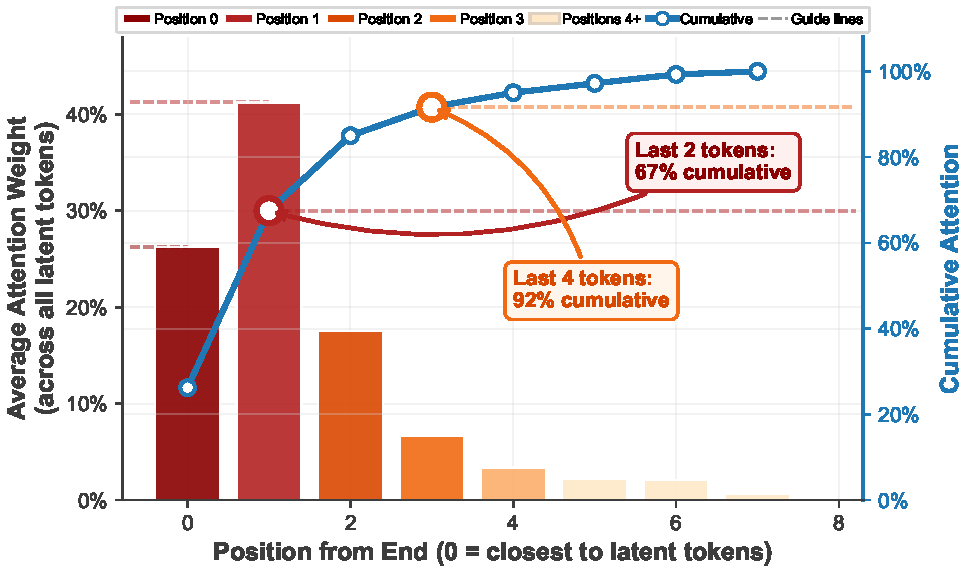
\includegraphics[width=\linewidth]{imgs/cross_attention_bias.pdf}
%   \caption{\textbf{Cross-attention concentrates on recent tokens.} Average attention weight as a function of position from the end of the prefix (0 = closest to the latent insertion point). Even with longer windows, attention mass concentrates on the last 1--2 hidden states, and cumulative attention saturates quickly.}
%   \label{fig:attention_heatmap}
% \end{figure}

% Table~\ref{tab:gpt2_gsm8k_context} shows that using the full prefix as cross-attention context degrades accuracy, while small windows remain strong. Figure~\ref{fig:attention_heatmap} explains this behavior: attention concentrates heavily on the most recent hidden states even when more context is available (e.g., $\sim$67\% mass on the last two tokens and $\sim$92\% on the last four). This supports the design choice of using a short window, which keeps latent synthesis lightweight without removing information the model actually uses.
% \textbf{[TODO: if you want a citation here, add one that supports ``recency dominance'' in autoregressive decoding; otherwise drop the sentence to avoid a weak citation.]}

% \subsection{Additional decoded latent examples}
% \label{app:more_examples}

% \begin{figure}[t]
% \centering
% \fbox{%
% \parbox{0.97\columnwidth}{
% \textbf{Example (Incorrect)} \hfill \textcolor{red}{\textbf{Incorrect}} \\[0.4em]
% \textbf{Question:} John cuts his grass to 2 inches. It grows 0.5 inches per month. When it gets to 4 inches he cuts it back down to 2 inches. It costs \$100 to get his grass cut. How much does he pay per year? \\[0.2em]
% \textbf{GT CoT:} $4{-}2=2 \rightarrow 2 \div 0.5 = 4$ months $\rightarrow 12 \div 4 = 3$ cuts $\rightarrow 100 \times 3 = 300$ \\[0.2em]
% \textbf{Predicted:} 200 \quad \textbf{GT:} 300 \\[0.4em]
% \begin{tabular}{c|cccccc}
% & L0 & L1 & L2 & L3 & L4 & L5 \\
% \hline
% Token & / & / & 200 & 200 & 200 & 5000 \\
% Prob  & 0.5\% & 0.4\% & 6.2\% & 11\% & 5.9\% & 8.5\% \\
% \end{tabular} \\[-0.2em]
% \textit{Interpretation:} Low and unstable confidence accompanies an incorrect reasoning trajectory; the final latent diverges.
% }}
% \caption{Additional decoded latent example supporting the qualitative trends discussed in Sec.~\ref{sec:latent_decoding}.}
% \label{fig:more_decoded_examples}
% \end{figure}

% \end{document}

\newpage
\appendix
\onecolumn


\section{Stability and initialization details}
\label{app:stability}

To stabilize optimization, we ground latent reasoning states in the task specification. Let $h_q$
denote the hidden state of the final question token. We initialize the output projection of the latent
synthesis cross-attention to zero and add $h_q$ as a residual to each latent state after synthesis.
This ensures that, at initialization, all latent states correspond to grounded copies of the question
representation and only deviate when learning discovers useful refinements.

This grounding serves two purposes: (i) it anchors latent reasoning to the task context throughout
training, and (ii) it prevents unstructured accumulation of latent history by ensuring that each
stage depends only on the current textual context and a fixed task representation.

\section{Attention masking and causal structure}
\label{app:masking}

We enforce the following attention constraints:
\begin{enumerate}
  \item Text tokens attend causally to earlier text tokens.
  \item Text tokens do not attend to future latent states.
  \item Latent states attend to all previous text tokens and to other latent states within the same
  stage bidirectionally.
  \item Answer tokens attend to all prior text tokens and all latent states from previous stages.
\end{enumerate}
This realizes a \emph{Text $\rightarrow$ Latents $\rightarrow$ Text} pattern while preserving
autoregressive decoding and preventing label leakage.

\section{PaCT training algorithm}
\label{app:algorithm}

Algorithm~\ref{alg:pact_training} provides the full curriculum training procedure for PaCT.

\begin{algorithm}[h]
\caption{Curriculum training for PaCT}
\label{alg:pact_training}
\begin{algorithmic}[1]
\Require Dataset $\mathcal{D}$, curriculum schedule $\{m_s,S_s\}$, slots $L$, parameters $\theta$, stepsize $\eta$
\For{$s=0,\dots,S_{\max}$}
  \For{$(q,r,a)\sim \mathcal{D}$}
    \State Replace first $m_s$ textual CoT tokens in $r$ with $S_s$ latent stages
    \State $x \leftarrow [\,q;\ \tilde{r}_s;\ a\,]$
    \State Compute $p_\theta(\cdot\mid x)$ and latent states $Z'^{(1:S_s)}$
    \State Update $\theta \leftarrow \theta - \eta \nabla_\theta \mathcal{L}(\theta)$
  \EndFor
\EndFor
\end{algorithmic}
\end{algorithm}

\section{Ablations on Latent Tokens}
\label{app:additional_results}

This section studies how PaCT utilizes latent tokens, with a focus on latent capacity and redundancy. In particular, we analyze (i) whether PaCT can outperform recurrent latent reasoning using fewer latent tokens, and (ii) whether multiple latent tokens within the same stage encode complementary or redundant information at inference time.

\subsection{Single-Latent PaCT vs.\ Dual-Latent Coconut}
\label{sec:single_double}
We first examine the minimum latent capacity required for effective continuous latent reasoning. Coconut relies on recurrent latent unrolling, where multiple latent tokens are generated sequentially and each latent must carry forward information from previous steps. In contrast, PaCT synthesizes latent tokens in parallel from the current context, without propagating latent states across steps.
\begin{table}[h]
    \centering
    \small
    \caption{Single-latent PaCT vs.\ dual-latent Coconut on GSM8k.}
    \label{tab:1v2}
    \begin{tabular}{lcc}
        \toprule
        Model & $c_{\text{thought}}$ & Accuracy (\%) \\
        \midrule
        PaCT    & 1 & 33.20 \\
        Coconut & 2 & 32.00 \\
        \bottomrule
    \end{tabular}
\end{table}
To isolate the effect of latent capacity, we compare PaCT using a single latent token per stage ($c_{\text{thought}}=1$) against Coconut using two recurrently unrolled latent tokens ($c_{\text{thought}}=2$), following standard Coconut settings on GSM8k. As shown in Table~\ref{tab:1v2}, PaCT with only one latent token already outperforms Coconut (33.20\% vs.\ 32.00\%).

This result indicates that PaCT does not rely on increased latent width to achieve strong performance. Instead, its stage-wise, context-grounded latent resynthesis produces more information-dense latent representations, allowing PaCT to match or exceed the performance of recurrent latent reasoning while using fewer latent tokens.

\subsection{Latent Redundancy Within Stages}
\label{subsec:latent_redundancy}
We investigate whether multiple latent tokens within the same PaCT stage encode complementary information or exhibit redundancy. We consider a PaCT model trained with two latent tokens per stage and three stages ($c_{\text{thought}}=2$, $S=3$), resulting in six latent tokens in total. At inference time, we selectively retain only one latent token per stage, discarding the other.
\begin{table}[h]
    \centering
    \small
    \caption{Accuracy when keeping only 1 of 2 latents per stage (PaCT trained with $c_{\text{thought}}=2$, $S=3$ on GSM8k).}
    \label{tab:latent_redundancy}
    \begin{tabular}{lcc}
        \toprule
        Configuration & \# Latents & Accuracy (\%) \\
        \midrule
        Full model & 6 & 34.4 \\
        First of each stage (L0, L2, L4) & 3 & 31.6 \\
        Second of each stage (L1, L3, L5) & 3 & 31.6 \\
        \bottomrule
    \end{tabular}
\end{table}

Table~\ref{tab:latent_redundancy} reports the resulting accuracy. Retaining either the first or the second latent token from each stage yields identical performance (31.6\%), regardless of which latent is kept. Although accuracy decreases relative to the full model (34.4\%), the symmetry across configurations indicates that latent tokens within the same stage encode largely redundant information.

This observation is consistent with the high within-stage similarity measured in our latent similarity analysis and supports the design choice of allocating compute toward greater depth (more stages) rather than increased latent width. In PaCT, reasoning benefits more from additional stages than from duplicating latent capacity within a stage.


\section{Latent decoding analysis -- extension}
\label{app:latent_decoding_examples}

This section provides additional qualitative evidence to complement the latent decoding analysis in Sec.~\ref{sec:latent_decoding}. Our goal is not to claim that latent reasoning states correspond to explicit natural language tokens, but rather to probe whether latent trajectories encode meaningful intermediate computations that align with the ground-truth reasoning process.

\begin{algorithm}[h ]
\caption{Top-$k$ Latent Decoding Probe for PaCT/Coconut ($k{=}5$)}
\label{alg:latent_probe_topk}
\begin{algorithmic}[1]
\Require Transformer $f_{\theta}$ with latent stages, output matrix $W_{\text{out}} \in \mathbb{R}^{|\mathcal{V}|\times d}$, input $x$, stages $S$
\Ensure Top-$k$ trajectories $\{(V_s, P_s)\}_{s=1}^{S}$
\State Compute latent embeddings $\{z_s \in \mathbb{R}^d\}_{s=1}^{S} \leftarrow f_{\theta}(x)$
\For{$s = 1, \ldots, S$}
    \State $\ell_s \leftarrow W_{\text{out}} z_s$
    \State $p_s \leftarrow \text{softmax}(\ell_s)$
    \State $V_s \leftarrow \text{top-}k(p_s)$, $P_s \leftarrow \{p_s(v) \mid v \in V_s\}$
\EndFor
\State \textbf{return} $\{(V_s, P_s)\}_{s=1}^{S}$
\end{algorithmic}
\end{algorithm}

We provide additional decoded latent trajectories to supplement Sec.~\ref{sec:latent_decoding}.


\paragraph{Top-$k$ latent decoding probe.}
We apply the Top-$k$ Latent Decoding Probe (Alg.~\ref{alg:latent_probe_topk}) to both PaCT and Coconut models. For each latent state, we project the latent embedding into vocabulary space using the output projection matrix and inspect the top-$k$ tokens along with their probabilities. This probe serves as a diagnostic tool to visualize how internal latent representations evolve across reasoning stages and whether they track intermediate quantities relevant to the final answer.

\paragraph{Progressive refinement in PaCT.}
Across correct examples (Examples S1--S2), PaCT exhibits a clear stage-wise progression from intermediate quantities toward the final answer. Early latent stages often decode to coarse intermediate values (e.g., partial sums or products), while later stages increasingly concentrate probability mass on the correct final answer. Importantly, latent pairs within the same stage frequently decode to identical tokens with similar probabilities, reflecting the high within-stage similarity reported in Table~4 of the main paper. This behavior is consistent with PaCT's design: latent states within a stage act as parallel hypotheses derived from the same contextual grounding, rather than representing sequential reasoning steps.

\vspace{0.8em}
\noindent\fbox{\parbox{0.97\textwidth}{
\textbf{Example S1} \hfill \textcolor{green!60!black}{\textbf{Correct}} \\[0.4em]
\textbf{Question:} Maggie went to Lou's aquarium and saw 100 goldfish. She was allowed to catch half, and she caught $3/5$ of that. How many remain to catch? \\[0.2em]
\textbf{Ground Truth CoT:} $100 \times \frac{1}{2} = 50 \rightarrow 50 \times \frac{3}{5} = 30 \rightarrow 50 - 30 = 20$ \\[0.2em]
\textbf{Predicted:} 20 \quad \textbf{GT:} 20 \\[0.4em]
\begin{tabular}{c|cccccc}
& L0 & L1 & L2 & L3 & L4 & L5 \\
\hline
Token & \textbf{50} & \textbf{50} & \textbf{30} & \textbf{30} & \textbf{20} & \textbf{20} \\
Prob  & 13\% & 14\% & 13\% & 20\% & 55\% & 56\% \\
\end{tabular} \\[-0.2em]
\textit{Interpretation:} Intermediate-to-final progression with sharpening confidence.
}}

\vspace{0.8em}
\noindent\fbox{\parbox{0.97\textwidth}{
\textbf{Example S2} \hfill \textcolor{green!60!black}{\textbf{Correct}} \\[0.4em]
\textbf{Question:} Mitchell has 8 packets of gum, 7 pieces each, and chews all but 2. How many does he chew? \\[0.2em]
\textbf{Ground Truth CoT:} $8 \times 7 = 56 \rightarrow 56 - 2 = 54$ \\[0.2em]
\textbf{Predicted:} 54 \quad \textbf{GT:} 54 \\[0.4em]
\begin{tabular}{c|cccccc}
& L0 & L1 & L2 & L3 & L4 & L5 \\
\hline
Token & \textbf{56} & \textbf{56} & \textbf{54} & \textbf{54} & \textbf{54} & \textbf{54} \\
Prob  & 5.2\% & 6.5\% & 25\% & 50\% & 87\% & 83\% \\
\end{tabular} \\[-0.2em]
\textit{Interpretation:} Answer emerges early and confidence sharpens across stages.
}}

\vspace{0.8em}
\noindent\fbox{\parbox{0.97\textwidth}{
\textbf{Example S3} \hfill \textcolor{red}{\textbf{Incorrect}} \\[0.4em]
\textbf{Question:} Roman and Remy used 33 gallons. Remy used $1$ more than $3\times$ Roman. How many did Remy use? \\[0.2em]
\textbf{Ground Truth CoT:} $x + (3x+1)=33 \rightarrow x=8 \rightarrow 3x+1=25$ \\[0.2em]
\textbf{Predicted:} 26.25 \quad \textbf{GT:} 25 \\[0.4em]
\begin{tabular}{c|cccccc}
& L0 & L1 & L2 & L3 & L4 & L5 \\
\hline
Token & 34 & 34 & 9 & 9 & \textbf{25} & \textbf{25} \\
Prob  & 11\% & 12\% & 7.5\% & 8.6\% & 22\% & 26\% \\
\end{tabular} \\[-0.2em]
\textit{Interpretation:} Latents reach the correct answer late, but decoding still commits to an incorrect output.
}}

\vspace{0.8em}
\noindent\fbox{\parbox{0.97\textwidth}{
\textbf{Example S4} \hfill \textcolor{red}{\textbf{Incorrect}} \\[0.4em]
\textbf{Question:} Suzy starts with 98 books. 43 checked out. Next day 23 returned and 5 checked out. Friday 7 returned. How many books? \\[0.2em]
\textbf{Ground Truth CoT:} $98-43=55 \rightarrow 55+23=78 \rightarrow 78-5=73 \rightarrow 73+7=80$ \\[0.2em]
\textbf{Predicted:} 119 \quad \textbf{GT:} 80 \\[0.4em]
\begin{tabular}{c|cccccc}
& L0 & L1 & L2 & L3 & L4 & L5 \\
\hline
Token & 69 & 69 & 76 & 72 & 70 & 70 \\
Prob  & 3.6\% & 3.4\% & 0.9\% & 1.6\% & 11\% & 9.3\% \\
\end{tabular} \\[-0.2em]
\textit{Interpretation:} Multi-step tracking fails; low probabilities reflect uncertainty.
}}

\vspace{0.8em}
\noindent\fbox{\parbox{0.97\textwidth}{
\textbf{Example S5} \hfill \textcolor{red}{\textbf{Incorrect}} \\[0.4em]
\textbf{Question:} Opera tickets increased from \$85 to \$102. What is the percent increase? \\[0.2em]
\textbf{Ground Truth CoT:} $102-85=17 \rightarrow \frac{17}{85}\times 100 = 20\%$ \\[0.2em]
\textbf{Predicted:} 12 \quad \textbf{GT:} 20 \\[0.4em]
\begin{tabular}{c|cccccc}
& L0 & L1 & L2 & L3 & L4 & L5 \\
\hline
Token & 73 & 73 & . & . & 12 & 12 \\
Prob  & 3.5\% & 3.1\% & 12\% & 18\% & 25\% & 24\% \\
\end{tabular} \\[-0.2em]
\textit{Interpretation:} Reasoning collapses; the model commits to an incorrect answer without computing the correct percentage.
}}

\paragraph{Failure modes and uncertainty signals.}
In incorrect cases (Examples S3--S5), the latent decoding probe reveals informative failure patterns. In some instances, PaCT latents reach the correct intermediate or even final value at later stages but fail to sustain sufficient confidence for correct decoding (Example S3). In others, the latent trajectory captures partial intermediates but fails to correctly compose them (Example S4), or collapses early to an incorrect estimate without completing the required computation (Example S5). These cases are characterized by low or diffuse probability mass across decoded tokens, indicating uncertainty rather than confident hallucination.

\paragraph{Comparison with Coconut.}
In contrast to PaCT, Coconut’s recurrently unrolled latent states exhibit less structured progression. Decoded tokens often fluctuate across stages, mix intermediate and irrelevant quantities, or prematurely terminate with end-of-text or non-numeric tokens. This behavior is consistent with Coconut’s recurrent latent propagation, where each latent must simultaneously carry forward prior information and perform new computation, leading to entangled representations and higher cross-stage similarity. As a result, Coconut latent trajectories are less interpretable and less aligned with the underlying arithmetic structure of the task.

Together, these extended examples reinforce three key observations. First, PaCT latent states encode meaningful intermediate quantities despite never being supervised to produce text. Second, reasoning in PaCT emerges as a stage-wise refinement process rather than a single evolving latent trajectory. Third, decoding probabilities provide a useful confidence signal: correct predictions are associated with sharpening probability mass on the final answer, while failures exhibit diffuse or unstable latent confidence. These findings support the claim that PaCT’s parallel, stage-wise latent resynthesis yields more structured and interpretable internal reasoning dynamics than recurrent latent unrolling.




\begin{figure}[t]
  \centering
  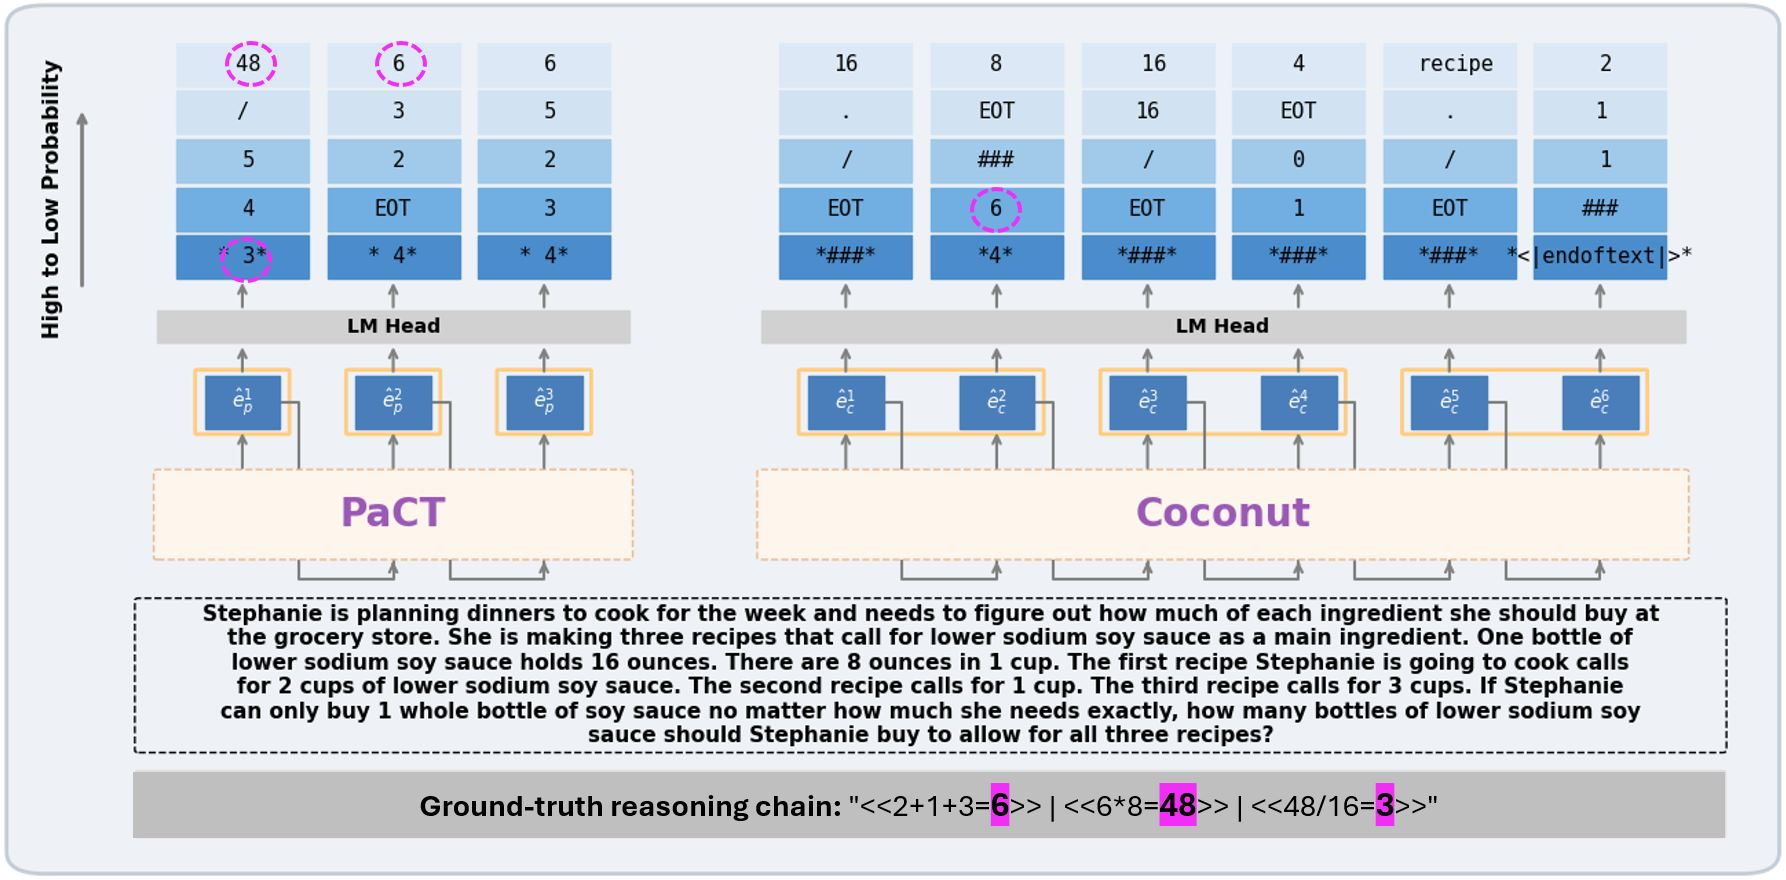
\includegraphics[width=\linewidth]{imgs/teaser2.JPG}
  \caption{\textbf{PaCT vs Coconut latent decoding comparison - example 1}}
  \label{fig:accuracy_and_latent_stages2}
\end{figure}

\begin{figure}[t]
  \centering
  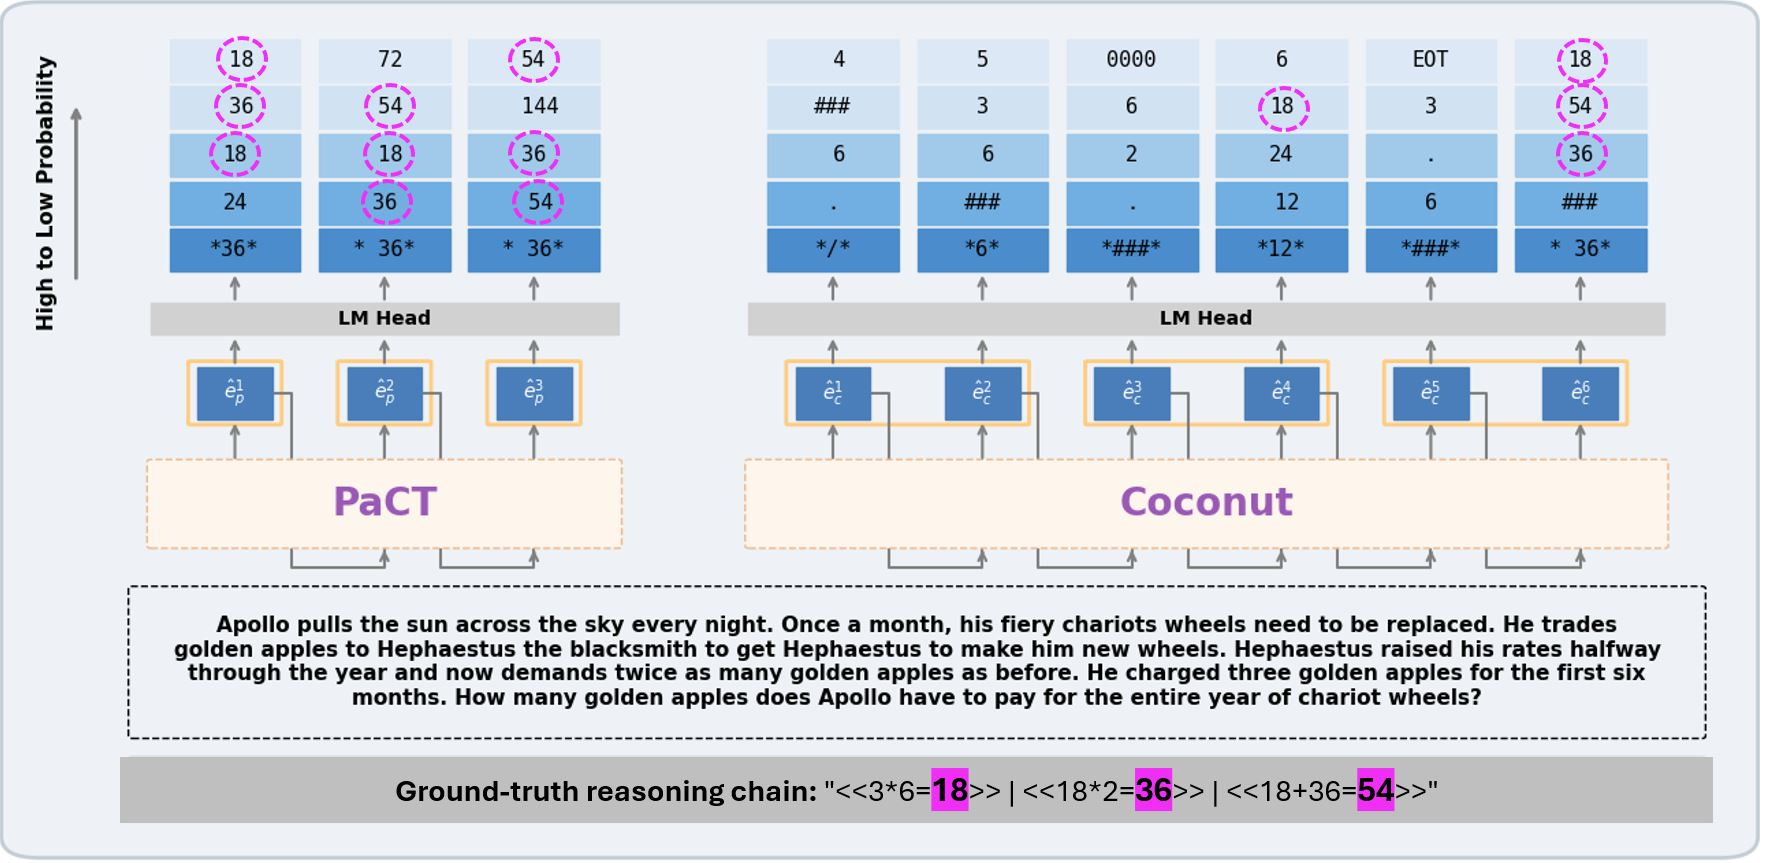
\includegraphics[width=\linewidth]{imgs/teaser3.JPG}
  \caption{\textbf{PaCT vs Coconut latent decoding comparison - example 2}}
  \label{fig:accuracy_and_latent_stages3}
\end{figure}

\begin{figure}[t]
  \centering
  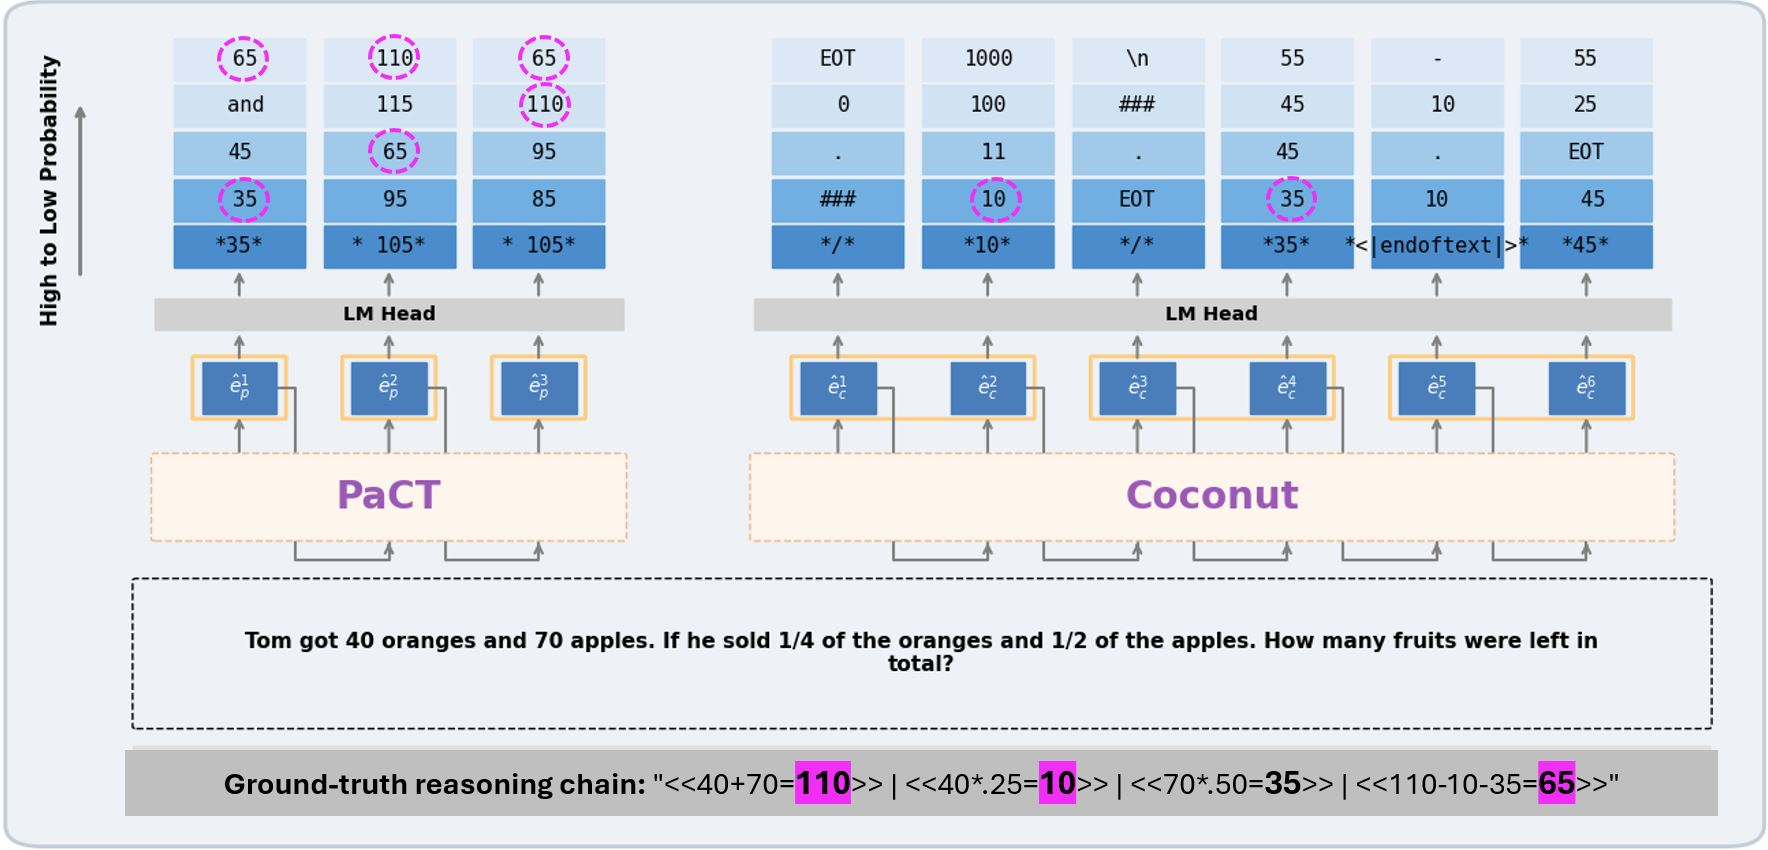
\includegraphics[width=\linewidth]{imgs/teaser4.JPG}
  \caption{\textbf{PaCT vs Coconut latent decoding comparison - example 3}}
  \label{fig:accuracy_and_latent_stages4}
\end{figure}



\section{Inference latency}
\label{sec:inference_latency}

\begin{figure}[t]
  \centering
  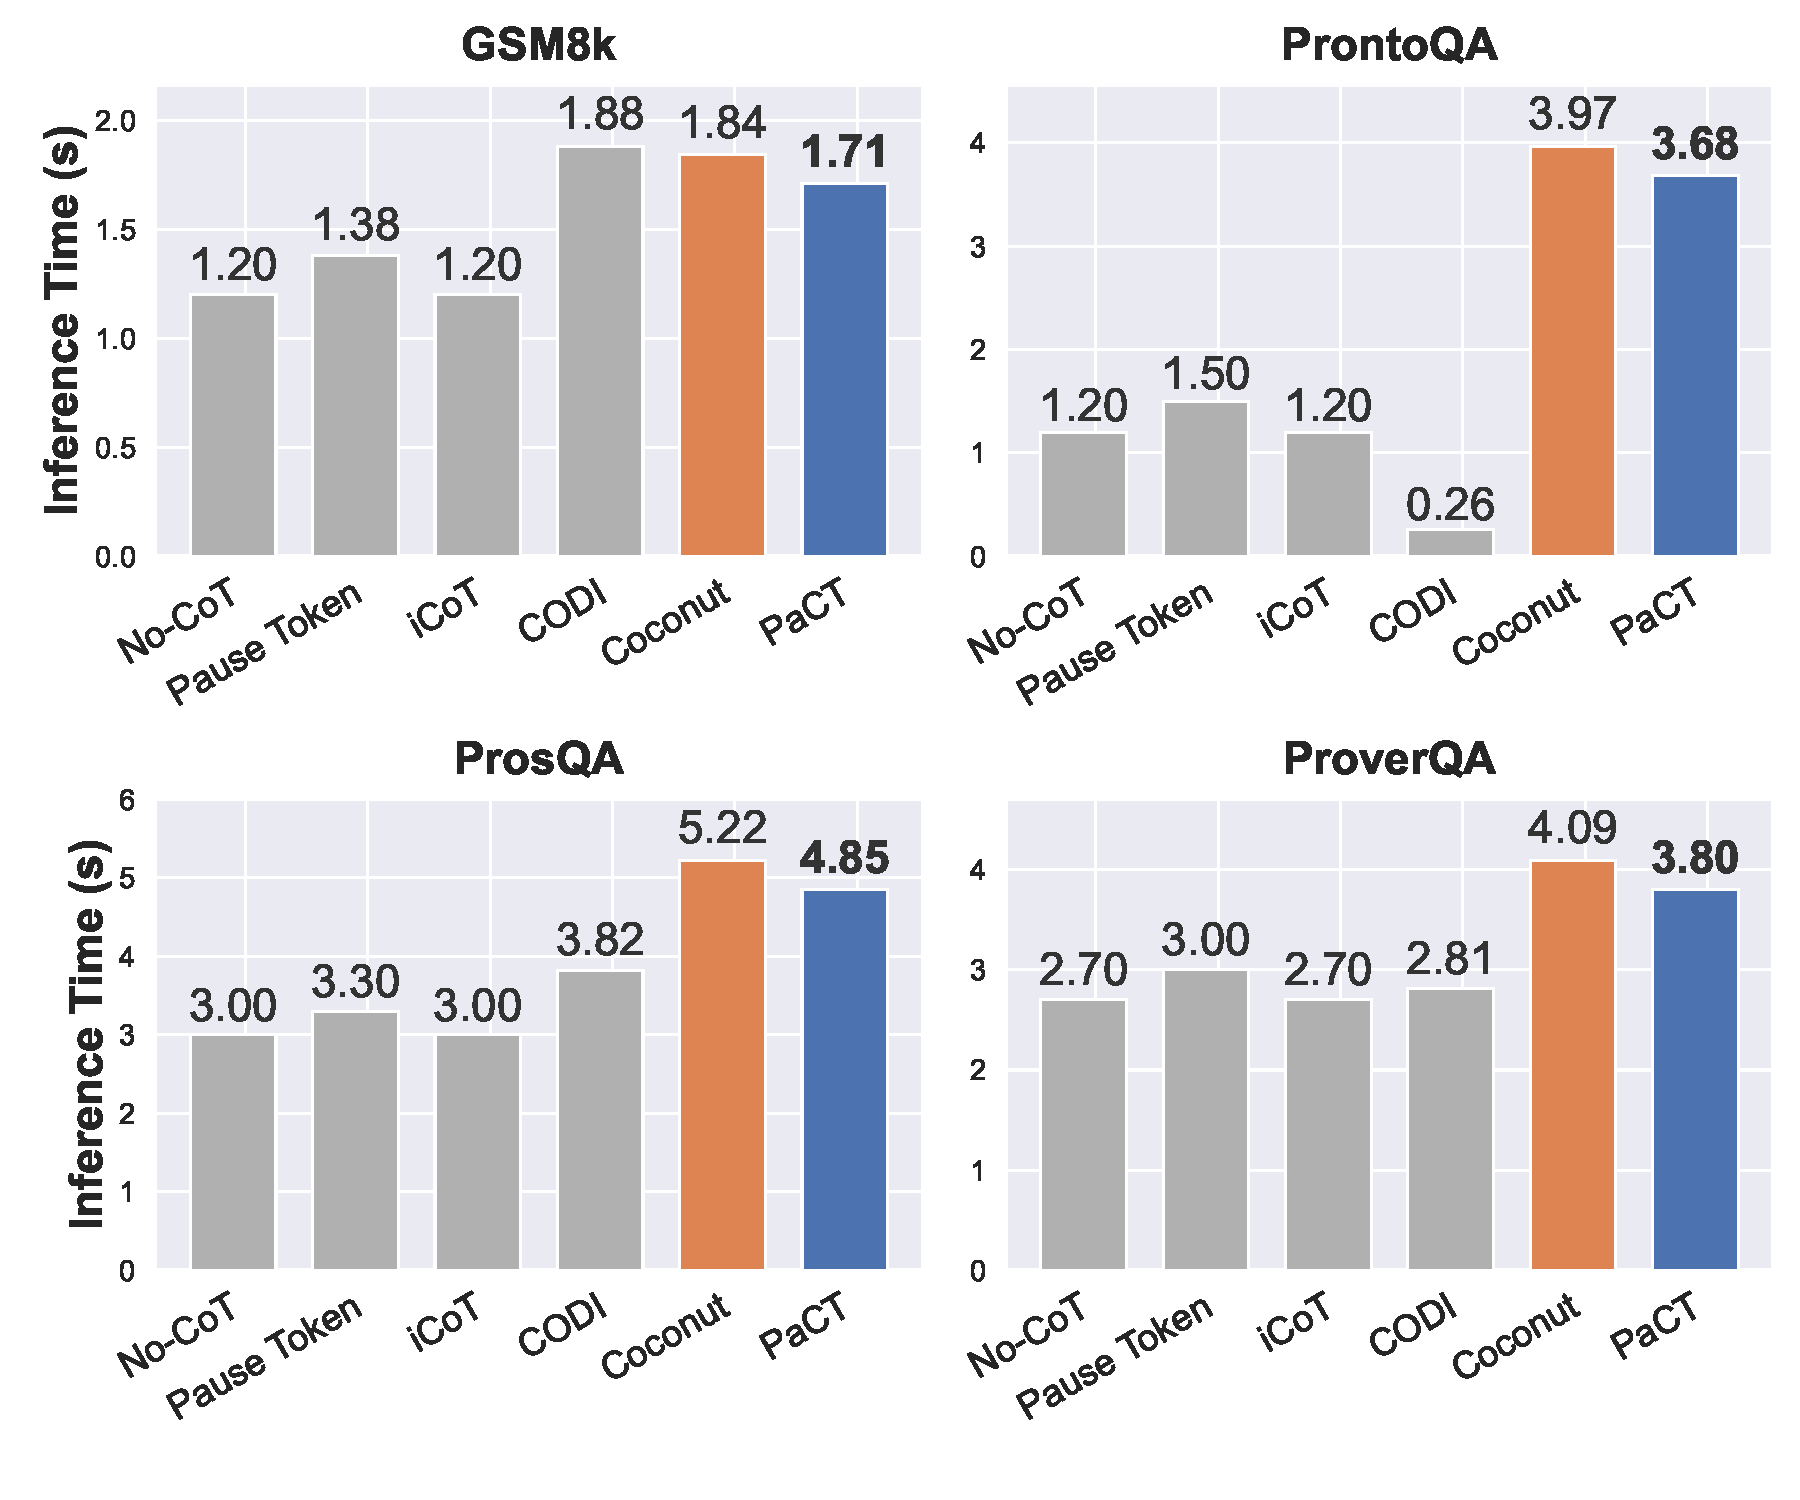
\includegraphics[width=\linewidth]{imgs/inference_times.pdf}
  \caption{\textbf{Inference time (seconds).} Inference time (per sample) for different reasoning methods across four benchmarks.
  PaCT reduces latency relative to Coconut by removing recurrent latent-unrolling overhead, while preserving competitive performance.
  }
  \label{fig:inference_time}
\end{figure}

Figure~\ref{fig:inference_time} reports inference time. PaCT is consistently faster than Coconut, though the
relative gain is smaller than for training because autoregressive answer decoding remains a dominant cost. This is an expected behavior as PaCT primarily removes serial dependence during latent generation; it does not change the causal decoding
interface for answer tokens.

\section{Source Code and Model Availability}
\label{sec:code_release}

To support reproducibility and facilitate future research, we release the full source code and trained model weights for PaCT. The repository includes training scripts, evaluation pipelines, and configuration files required to reproduce all experiments reported in this paper.

Our implementation and pretrained models are publicly available at:
\begin{center}
\href{https://anonymous.4open.science/r/pact-576C/}{\texttt{https://anonymous.4open.science/r/pact-576C/}}
\end{center}




% \subsection{Robustness to perturbations in early latent states}
% \label{sec:latent_robustness}

% Our latent similarity analysis (Table~\ref{tab:latent_similarity}) shows a clear structural difference between PaCT and
% Coconut: PaCT exhibits low cross-stage similarity, indicating stage-wise specialization, while Coconut exhibits high
% cross-stage similarity, suggesting that information is tightly coupled and propagated across latent steps. This motivates
% a robustness test: \emph{if early latent states are perturbed, methods with stronger cross-stage coupling should be more
% sensitive, as errors are carried forward through the latent trajectory.}

% \paragraph{Setup.}
% We evaluate robustness by perturbing only the \emph{first} latent stage at inference time and measuring the resulting
% change in answer accuracy. Let $Z^{(1)} \in \mathbb{R}^{L \times d}$ denote the stage-1 latent states. We consider two
% perturbations: (i) \textbf{additive Gaussian noise}, $\tilde{Z}^{(1)} = Z^{(1)} + \sigma \epsilon$ with
% $\epsilon \sim \mathcal{N}(0, I)$, and (ii) \textbf{magnitude scaling}, $\tilde{Z}^{(1)} = \alpha Z^{(1)}$.
% All subsequent latent stages are computed normally, using the perturbed stage-1 interface.

% \begin{table}[t]
% \centering
% \small
% \caption{\textbf{Robustness to perturbing the first latent stage.} Accuracy (\%) under stage-1 latent perturbations.
% PaCT exhibits smaller degradation than Coconut, consistent with reduced cross-stage coupling.}
% \label{tab:latent_perturbation_robustness}
% \begin{tabular}{lccc}
% \toprule
% Method & Clean & Gaussian ($\sigma{=}0.05$) & Scale ($\alpha{=}0.8$) \\
% \midrule
% Coconut & 32.0 $\pm$ 1.5 & 27.4 $\pm$ 1.7 & 29.8 $\pm$ 1.6 \\
% PaCT    & 34.4 $\pm$ 0.1 & 33.1 $\pm$ 0.2 & 33.6 $\pm$ 0.2 \\
% \bottomrule
% \end{tabular}
% \end{table}

% As shown in Table~\ref{tab:latent_perturbation_robustness}, perturbing the first latent stage leads to a substantially
% larger accuracy drop for Coconut than for PaCT. This aligns with the similarity analysis: Coconut’s higher cross-stage
% similarity indicates that latent states are more tightly coupled, so perturbations introduced early are propagated and
% amplified through recurrent unrolling. In contrast, PaCT’s stage-wise resynthesis yields weaker cross-stage dependence,
% allowing later stages to re-ground latent computation in context and partially correct early perturbations. These results
% provide additional evidence that PaCT’s parallel, non-recurrent latent design improves not only efficiency but also the
% stability of latent reasoning.



% \begin{table}[t]
% \centering
% \begin{tabular}{lcc}
% \toprule
% Method & Peak VRAM (GB) & TFLOPS \\
% \midrule
% Coconut    & 21 &  \\
% CoLaR      & 20 & 11.5 \\
% CODI       & -- &  \\
% \textbf{PaCT} & 28 &  \\
% \bottomrule
% \end{tabular}
% \caption{\textbf{Peak GPU memory usage on a single dataset.}
% Peak VRAM is measured during training for one dataset under a fixed hardware and batch-size configuration.}
% \label{tab:vram_usage}
% \end{table}




\end{document}
% This document was modified from the file originally made available by
% Pat Langley and Andrea Danyluk for ICML-2K. This version was created
% by Iain Murray in 2018, and modified by Alexandre Bouchard in
% 2019 and 2021 and by Csaba Szepesvari, Gang Niu and Sivan Sabato in 2022.
% Modified again in 2023 and 2024 by Sivan Sabato and Jonathan Scarlett.
% Previous contributors include Dan Roy, Lise Getoor and Tobias
% Scheffer, which was slightly modified from the 2010 version by
% Thorsten Joachims & Johannes Fuernkranz, slightly modified from the
% 2009 version by Kiri Wagstaff and Sam Roweis's 2008 version, which is
% slightly modified from Prasad Tadepalli's 2007 version which is a
% lightly changed version of the previous year's version by Andrew
% Moore, which was in turn edited from those of Kristian Kersting and
% Codrina Lauth. Alex Smola contributed to the algorithmic style files.


